\documentclass[12pt]{article}

\textwidth 16cm \textheight 23cm \evensidemargin 0cm
\oddsidemargin 0cm \topmargin -2cm
\parindent 0pt
\parskip \medskipamount


\usepackage[dutch]{babel}
\usepackage{amssymb}
\usepackage{amsmath}
\usepackage[utf8,latin1]{inputenc}
\usepackage[normalem]{ulem} % strikethrough normal text with \sout{text}
\usepackage{cancel} % strikethrough in math mode with \cancel{text}
%\usepackage{gensymb}

\usepackage{subfig}
\usepackage{wrapfig}
\usepackage{graphicx}
\usepackage{graphics}
\usepackage{latexsym}
%\usepackage[latin1]{inputenc} %letters met accenten mogen in broncode gebruikt worden
\usepackage{amssymb,amsmath,amsthm} %allerlei wiskundige symbolen => http://www.ams.org/tex/amslatex.html voor read-me's
%\usepackage[small,bf,hang]{caption}
\usepackage[table]{xcolor}
\usepackage{pgf,tikz}
\usetikzlibrary{arrows}

\usepackage[pdftex]{hyperref} 
\hypersetup{setpagesize=false}
%\hypersetup{bookmarksopen}
\hypersetup{bookmarksnumbered} %voor de bookmarks in pdf de nrs zetten ook
\hypersetup{pdfborder=0.1pt} %de rand rond de links smaller maken
\hypersetup{linktocpage=true} %titels of pgnrs omkaderen in toc
\hypersetup{colorlinks=true} %kaders rond links of tekst in kleur, kaders gaan weg bij afprinten, kleur blijft


\numberwithin{equation}{section} %om de equations labels te geven die met section meegaan, dus niet gwn (1) (2) ... maar (1.1) (1.2) ...

%iets voor modulonotatie
\makeatletter
\def\imod#1{\allowbreak\mkern10mu({\operator@font mod}\,\,#1)}
\makeatother

%Getallenverzamelingen
\newcommand{\N}{\mathbb{N}}
\newcommand{\Z}{\mathbb{Z}}
\newcommand{\Q}{\mathbb{Q}}
\newcommand{\R}{\mathbb{R}}
\newcommand{\C}{\mathbb{C}}
\newcommand{\mO}{\mathcal{O}}
%<= en >= mooier maken
\renewcommand{\leq}{\leqslant}
\renewcommand{\geq}{\geqslant}

%speciale wiskunde letters: \mathcal{} of \mathfrak{}

%Nieuwe omgevingen voor definities en stellingen
\theoremstyle{plain}  \newtheorem{stel}{Stelling}[section]
\theoremstyle{plain}  \newtheorem{lemma}[stel]{Lemma}
\theoremstyle{plain}  \newtheorem{gevolg}[stel]{Gevolg}
\theoremstyle{definition}  \newtheorem{defi}[stel]{Definitie}
\theoremstyle{definition} \newtheorem{vb}[stel]{Voorbeeld}
\theoremstyle{definition} \newtheorem{vbn}[stel]{Voorbeelden}
\theoremstyle{definition}  \newtheorem{opm}[stel]{Opmerking}
\theoremstyle{plain}  \newtheorem{opdracht}{Opdracht}

\hyphenation{e-ner-zijds}
\hyphenation{ka-nons-ko-gel}
\hyphenation{schrij-ven}
\hyphenation{ka-nons-ko-gels}
\hyphenation{ont-stond}
\hyphenation{kwa-dra-tisch}

\usepackage{color}
\newcommand{\todo}[1]{\textcolor{red}{\##1\#}}
\newcommand{\question}[1]{\textcolor{blue}{\##1\#}}

% Wissel tussen versie van leerkracht en versie voor leerlingen
% gebruik: \teacher{Dit is een notitie voor de leerkracht}
% eerste parameter is de notitie
\newcommand{\teacher}[1]{\textcolor{gray}{\emph{#1}}}
%\newcommand{\teacher}[1]{}

% Wissel tussen versie van leerkracht en versie voor leerling door antwoorden te verbergen
% gebruik: \answer[2cm]{Dit is een antwoord}
% tussen vierkante haakjes is optioneel de lengte die voorzien moet worden (default = 0cm),
% de parameter is het antwoord
\newcommand{\answer}[2][0cm]{{\textcolor{gray}{\emph{#2}}}}
%\newcommand{\answer}[2][0cm]{\vspace*{#1}}

\newcommand{\ask}[1]{\underline{\bf Vraag:} #1}
\newcommand{\task}[1]{\underline{\bf Opdracht:} #1}

\graphicspath{{figuren/}}

%\newtheorem{definitie}{Definitie}

\newcommand{\degree}{\ensuremath{^\circ}}

\begin{document}

\thispagestyle{empty}

\begin{center}
  \begin{minipage}{7cm}
    \begin{center}

      
\includegraphics[width=5cm]{ruglogo.pdf}

      {\large
      Universiteit Gent \\
      Faculteit  Wetenschappen \\
      Vakgroep  Wiskunde
      } 
    \end{center}
  \end{minipage}

  \vspace{3cm}

  {\Huge\bf 
  Vullen van Vlakken en Volumes
  }
  
  \baselineskip=12pt
  \vspace{1.5cm}

  {\large\bf  Lien Lambert }\\
  \vspace{0.5cm}
  {\large \bf Pieter Pareit }\\
  \vspace{0.5cm}
  {\large \bf Jordy Vanpoucke}\\

  \baselineskip=12pt

  \vspace{2cm}

  \bigskip

  {\large Academiejaar 2011-2012}

\end{center}

\vfill

\hspace*{\fill}
\begin{minipage}{8cm}
\noindent   Project Vakdidactiek Wiskunde II
\end{minipage}

  \bigskip

  \hspace*{\fill}
  \begin{minipage}{8cm}
  \noindent  Prof. Dr.  F. De Clerck\\
  Praktijkassistent G. Maes
\end{minipage}

\newpage
\tableofcontents 
\newpage


%\section{Vullen van Vlakken en Volumes ({\sc $V^3$})}
\section{Inleiding}

\subsection{Kennismaking met het vullen van vlakken}
Als introductie op deze lessenreeks over het vullen van vlakken en volumes, zullen we eens klassikaal nagaan wat dit onderwerp precies inhoudt. Om te beginnen zullen we op zoek gaan naar een goede definitie van een vlakvulling. Als we het begrip `vlakvulling' ingeven op een zoekmachine, dan vinden we een groot aantal afbeeldingen. Onder andere komen we terecht bij de volgende afbeeldingen van vlakvullingen.
\begin{figure}[h]
  \centering
  \subfloat[]{
\includegraphics[height=4.8cm]{tess5}}
  \subfloat[]{
\includegraphics[height=4.8cm]{escher2}}
  \subfloat[]{
\includegraphics[height=4.8cm]{tess104}}\\
\end{figure}\\
Op deze drie afbeeldingen zien we vlakvullingen van Escher. Hier zullen we later nog op ingaan.\\
We zullen nu zelf op zoek gaan naar figuren om een vlak te vullen.\\ 
\ask{Welke eenvoudige meetkundige vlakke figuren kennen jullie?}\\
\answer{Rechthoek, vierkant, driehoek, cirkel, \ldots}\\
\teacher{De leerlingen kunnen hier veel verschillende antwoorden geven, maar zullen waarschijnlijk wel komen tot de bovenstaande antwoorden.}\\
We zullen nu eens kijken hoe we een vlak volledig kunnen vullen met deze figuren aan de hand van translaties en/of rotaties. In theorie kunnen we een vlak vullen met verschillende soorten figuren, maar om het eenvoudig te houden zullen we in dit lessenpakket kijken hoe we een vlak kunnen vullen met identieke figuren.\\
\ask{Welke beperkingen moeten nog opleggen opdat iets een vlakvulling is? Als we nu het vlak willen vullen met identieke figuren mogen deze figuren dan overlappen?}\\
\teacher{Laat eerst zelf vragen en opmerkingen opkomen bij de leerlingen De leerlingen kunnen ook redeneren waarom dit zo is.}\\
Zo komen we dus tot de volgende definitie van een vlakvulling:\\
\answer{Een \textbf{vlakvulling} is een vulling van het vlak met figuren, waarbij er geen gaten mogen zijn en de figuren niet mogen overlappen.}\\
We kunnen nu proberen om een oneindig groot vlak zo optimaal mogelijk te vullen met identieke figuren.\\
\ask{Is het altijd mogelijk om een oneindig groot vlak compleet te vullen?}\\
\answer{Neen}\\
Daarom maken we dus het onderscheid tussen twee definities. Enerzijds zullen we spreken over een \textbf{complete vlakvulling} als we een oneindig vlak volledig kunnen vullen met een bepaalde figuur aan de hand van translaties en/of rotaties. Anderzijds zullen we spreken over een \textbf{optimale vlakvulling} als we het oneindig grote vlak zo compleet mogelijk kunnen vullen. Bij optimale vlakvullingen zullen we ook spreken over de \textbf{effici\"{e}ntie} van de vlakvulling. Deze effici\"{e}ntie drukken we uit in een percentage. Als de effici\"{e}ntie van de optimale vlakvulling dus gelijk is aan $100\%$, dan hebben we een complete vlakvulling.
\subsection{Vullen van een oneindig groot vlak}
Om te beginnen kunnen we nu eens kijken hoe we een vlak compleet kunnen vullen met figuren, meer bepaald zullen we proberen het vlak te vullen met regelmatige veelhoeken. Het compleet vullen van een vlak met regelmatige veelhoeken noemen we ook een regulier vlakvulling of regulier betegeling. Eerst zullen we nu eens nadenken over de volgende vragen.\\
\teacher{Op dit punt verdelen we de leerlingen in groepjes en delen we aan de leerlingen identieke figuren uit die uitgeknipt werden in karton. Elk groepje krijgt een stapel identieke regelmatige driehoeken, een stapel identieke regelmatige vierhoeken, een stapel identieke regelmatige vijfhoeken, een stapel identieke regelmatige zeshoeken, een stapel identieke regelmatige zevenhoeken en een stapel identieke regelmatige achthoeken.}\\
\task{Probeer eens uit te zoeken met welke regelmatige veelhoeken je een complete vlakvulling kan maken.}\\
\teacher{De leerlingen proberen in groepjes de tafels volledig te vullen met deze kartonnen regelmatige veelhoeken en zullen zo tot bevindingen komen.}\\
\answer{Een complete vlakvulling is enkel mogelijk met regelmatige driehoeken, regelmatige vierhoeken en regelmatige zeshoeken.}\\
\ask{Hoe komt het dat een complete vlakvulling met andere regelmatige veelhoeken niet lukt?}\\
\answer{We zien dat bij de vlakvulling met regelmatige veelhoeken de hoeken van ieder toppunt precies moeten passen omdat we anders gaten of overlappingen hebben. De grootte van de binnenhoeken van de regelmatige veelhoeken moet dus een deler zijn van 360.}\\
We zullen nu onze bevindingen wiskundig correct proberen te formuleren en bewijzen. Laat ons eerst een antwoord vinden op de volgende vragen.\\
\ask{
\begin{itemize}
\item Kan je een formule vinden voor de som van de binnenhoeken van een regelmatige $n-$hoek?\\
\item Kan je een formule vinden voor de grootte van de binnenhoeken van een regelmatige $n-$hoek?\\
\item Dus de grootte van de binnenhoeken van een regelmatige driehoek is gelijk aan? \answer{$60\degree$}\\
\item Dus de grootte van de binnenhoeken van een regelmatige vierhoek is gelijk aan? \answer{$90\degree$}\\
\item Dus de grootte van de binnenhoeken van een regelmatige vijfhoek is gelijk aan? \answer{$108\degree$}\\
\item \ldots
\end{itemize}}
\teacher{We komen tot de volgende stelling, `Als we een oneindig groot vlak compleet willen vullen met regelmatige veelhoeken dan lukt dit enkel met regelmatige driehoeken, regelmatige vierhoeken en regelmatige zeshoeken'}\\
\teacher{Bewijs: De som van de binnenhoeken van een $n$-hoek is $180\degree(n-2)$. Omdat een regelmatige $n$-hoek $n$ hoeken heeft is dus de grootte van \'{e}\'{e}n binnenhoek gelijk aan $\frac{180\degree(n-2)}{n} = 180\degree(1-\frac{2}{n})$. Als we $r$ regelmatige $n$-hoeken plaatsen op \'{e}\'{e}n punt, zodanig dat ze niet overlappen en geen gaten laten, dan moet de som van alle binnenhoeken gelijk zijn aan $360\degree$.\\We krijgen dus de volgende identiteit: $$r\cdot 180\degree(1-\frac{2}{n}) = 360\degree \;.$$ Dit kan vereenvoudigd worden tot $$n = \frac{2r}{r-2}\;.$$ Omdat $n$, het aantal hoekpunten van de regelmatige veelhoek, zeker positief moet zijn, volgt alvast dat $r\geq 3$. Omdat de veelhoek met het kleinste aantal hoekpunten de driehoek is, hebben we $n\geq 3$ en volgt er dus dat $r\leq 6$. Vullen we nu $r = 3, 4, 5 \mbox{ en } 6$ in, dan krijgen we $n=6,4,\frac{10}{3} \mbox{ en } 3$. Het nummer $n$ is een natuurlijk getal, dus $n= 6, 4 \mbox{ en } 3$ zijn mogelijk. Ofwel, enkel regelmatige zeshoeken, regelmatige vierhoeken of regelmatige driehoeken kunnen een oneindig groot vlak compleet opvullen.}
\begin{figure}[ht]
  \centering
  \subfloat[Regelmatige driehoeken]{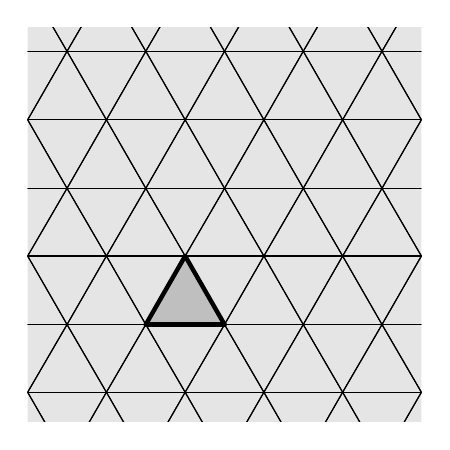
\begin{tikzpicture}[line cap=round,line join=round,>=triangle 45,x=1.0cm,y=1.0cm]
\clip(0.5,0.5) rectangle (5.5,5.5);
\fill[fill=black,fill opacity=0.1] (0,0) -- (1,0) -- (0.5,0.87) -- cycle;
\fill[fill=black,fill opacity=0.1] (0.5,0.87) -- (1,0) -- (1.5,0.87) -- cycle;
\fill[fill=black,fill opacity=0.1] (1,0) -- (2,0) -- (1.5,0.87) -- cycle;
\fill[fill=black,fill opacity=0.1] (1.5,0.87) -- (2,0) -- (2.5,0.87) -- cycle;
\fill[fill=black,fill opacity=0.1] (2,0) -- (3,0) -- (2.5,0.87) -- cycle;
\fill[fill=black,fill opacity=0.1] (2.5,0.87) -- (3,0) -- (3.5,0.87) -- cycle;
\fill[fill=black,fill opacity=0.1] (3,0) -- (4,0) -- (3.5,0.87) -- cycle;
\fill[fill=black,fill opacity=0.1] (3.5,0.87) -- (4,0) -- (4.5,0.87) -- cycle;
\fill[fill=black,fill opacity=0.1] (4,0) -- (5,0) -- (4.5,0.87) -- cycle;
\fill[fill=black,fill opacity=0.1] (4.5,0.87) -- (5,0) -- (5.5,0.87) -- cycle;
\fill[fill=black,fill opacity=0.1] (5,0) -- (6,0) -- (5.5,0.87) -- cycle;
\fill[fill=black,fill opacity=0.1] (5.5,0.87) -- (6,0) -- (6.5,0.87) -- cycle;
\fill[fill=black,fill opacity=0.1] (6,0) -- (7,0) -- (6.5,0.87) -- cycle;
\fill[fill=black,fill opacity=0.1] (6.5,0.87) -- (7,0) -- (7.5,0.87) -- cycle;
\fill[fill=black,fill opacity=0.1] (7,0) -- (8,0) -- (7.5,0.87) -- cycle;
\fill[fill=black,fill opacity=0.1] (7.5,0.87) -- (8,0) -- (8.5,0.87) -- cycle;
\fill[fill=black,fill opacity=0.1] (8,0) -- (9,0) -- (8.5,0.87) -- cycle;
\fill[fill=black,fill opacity=0.1] (8.5,0.87) -- (9,0) -- (9.5,0.87) -- cycle;
\fill[fill=black,fill opacity=0.1] (9,0) -- (10,0) -- (9.5,0.87) -- cycle;
\fill[fill=black,fill opacity=0.1] (9.5,0.87) -- (10,0) -- (10.5,0.87) -- cycle;
\fill[fill=black,fill opacity=0.1] (0,1.73) -- (0.5,0.87) -- (1,1.73) -- cycle;
\fill[fill=black,fill opacity=0.1] (0.5,0.87) -- (1.5,0.87) -- (1,1.73) -- cycle;
\fill[fill=black,fill opacity=0.1] (1,1.73) -- (1.5,0.87) -- (2,1.73) -- cycle;
\fill[fill=black,fill opacity=0.1] (1.5,0.87) -- (2.5,0.87) -- (2,1.73) -- cycle;
\fill[fill=black,fill opacity=0.1] (2,1.73) -- (2.5,0.87) -- (3,1.73) -- cycle;
\fill[fill=black,fill opacity=0.1] (2.5,0.87) -- (3.5,0.87) -- (3,1.73) -- cycle;
\fill[fill=black,fill opacity=0.1] (3,1.73) -- (3.5,0.87) -- (4,1.73) -- cycle;
\fill[fill=black,fill opacity=0.1] (3.5,0.87) -- (4.5,0.87) -- (4,1.73) -- cycle;
\fill[fill=black,fill opacity=0.1] (4,1.73) -- (4.5,0.87) -- (5,1.73) -- cycle;
\fill[fill=black,fill opacity=0.1] (4.5,0.87) -- (5.5,0.87) -- (5,1.73) -- cycle;
\fill[fill=black,fill opacity=0.1] (5,1.73) -- (5.5,0.87) -- (6,1.73) -- cycle;
\fill[fill=black,fill opacity=0.1] (5.5,0.87) -- (6.5,0.87) -- (6,1.73) -- cycle;
\fill[fill=black,fill opacity=0.1] (6,1.73) -- (6.5,0.87) -- (7,1.73) -- cycle;
\fill[fill=black,fill opacity=0.1] (6.5,0.87) -- (7.5,0.87) -- (7,1.73) -- cycle;
\fill[fill=black,fill opacity=0.1] (7,1.73) -- (7.5,0.87) -- (8,1.73) -- cycle;
\fill[fill=black,fill opacity=0.1] (7.5,0.87) -- (8.5,0.87) -- (8,1.73) -- cycle;
\fill[fill=black,fill opacity=0.1] (8,1.73) -- (8.5,0.87) -- (9,1.73) -- cycle;
\fill[fill=black,fill opacity=0.1] (8.5,0.87) -- (9.5,0.87) -- (9,1.73) -- cycle;
\fill[fill=black,fill opacity=0.1] (9,1.73) -- (9.5,0.87) -- (10,1.73) -- cycle;
\fill[fill=black,fill opacity=0.1] (9.5,0.87) -- (10.5,0.87) -- (10,1.73) -- cycle;
\fill[fill=black,fill opacity=0.1] (0,1.73) -- (1,1.73) -- (0.5,2.6) -- cycle;
\fill[fill=black,fill opacity=0.1] (0.5,2.6) -- (1,1.73) -- (1.5,2.6) -- cycle;
\fill[fill=black,fill opacity=0.1] (1,1.73) -- (2,1.73) -- (1.5,2.6) -- cycle;
\fill[fill=black,fill opacity=0.1] (1.5,2.6) -- (2,1.73) -- (2.5,2.6) -- cycle;
\fill[line width=1.6pt,fill=black,fill opacity=0.25] (2,1.73) -- (3,1.73) -- (2.5,2.6) -- cycle;
\fill[fill=black,fill opacity=0.1] (2.5,2.6) -- (3,1.73) -- (3.5,2.6) -- cycle;
\fill[fill=black,fill opacity=0.1] (3,1.73) -- (4,1.73) -- (3.5,2.6) -- cycle;
\fill[fill=black,fill opacity=0.1] (3.5,2.6) -- (4,1.73) -- (4.5,2.6) -- cycle;
\fill[fill=black,fill opacity=0.1] (4,1.73) -- (5,1.73) -- (4.5,2.6) -- cycle;
\fill[fill=black,fill opacity=0.1] (4.5,2.6) -- (5,1.73) -- (5.5,2.6) -- cycle;
\fill[fill=black,fill opacity=0.1] (5,1.73) -- (6,1.73) -- (5.5,2.6) -- cycle;
\fill[fill=black,fill opacity=0.1] (5.5,2.6) -- (6,1.73) -- (6.5,2.6) -- cycle;
\fill[fill=black,fill opacity=0.1] (6,1.73) -- (7,1.73) -- (6.5,2.6) -- cycle;
\fill[fill=black,fill opacity=0.1] (6.5,2.6) -- (7,1.73) -- (7.5,2.6) -- cycle;
\fill[fill=black,fill opacity=0.1] (7,1.73) -- (8,1.73) -- (7.5,2.6) -- cycle;
\fill[fill=black,fill opacity=0.1] (7.5,2.6) -- (8,1.73) -- (8.5,2.6) -- cycle;
\fill[fill=black,fill opacity=0.1] (8,1.73) -- (9,1.73) -- (8.5,2.6) -- cycle;
\fill[fill=black,fill opacity=0.1] (8.5,2.6) -- (9,1.73) -- (9.5,2.6) -- cycle;
\fill[fill=black,fill opacity=0.1] (9,1.73) -- (10,1.73) -- (9.5,2.6) -- cycle;
\fill[fill=black,fill opacity=0.1] (9.5,2.6) -- (10,1.73) -- (10.5,2.6) -- cycle;
\fill[fill=black,fill opacity=0.1] (0,3.46) -- (0.5,2.6) -- (1,3.46) -- cycle;
\fill[fill=black,fill opacity=0.1] (0.5,2.6) -- (1.5,2.6) -- (1,3.46) -- cycle;
\fill[fill=black,fill opacity=0.1] (1,3.46) -- (1.5,2.6) -- (2,3.46) -- cycle;
\fill[fill=black,fill opacity=0.1] (1.5,2.6) -- (2.5,2.6) -- (2,3.46) -- cycle;
\fill[fill=black,fill opacity=0.1] (2,3.46) -- (2.5,2.6) -- (3,3.46) -- cycle;
\fill[fill=black,fill opacity=0.1] (2.5,2.6) -- (3.5,2.6) -- (3,3.46) -- cycle;
\fill[fill=black,fill opacity=0.1] (3,3.46) -- (3.5,2.6) -- (4,3.46) -- cycle;
\fill[fill=black,fill opacity=0.1] (3.5,2.6) -- (4.5,2.6) -- (4,3.46) -- cycle;
\fill[fill=black,fill opacity=0.1] (4,3.46) -- (4.5,2.6) -- (5,3.46) -- cycle;
\fill[fill=black,fill opacity=0.1] (4.5,2.6) -- (5.5,2.6) -- (5,3.46) -- cycle;
\fill[fill=black,fill opacity=0.1] (5,3.46) -- (5.5,2.6) -- (6,3.46) -- cycle;
\fill[fill=black,fill opacity=0.1] (5.5,2.6) -- (6.5,2.6) -- (6,3.46) -- cycle;
\fill[fill=black,fill opacity=0.1] (6,3.46) -- (6.5,2.6) -- (7,3.46) -- cycle;
\fill[fill=black,fill opacity=0.1] (6.5,2.6) -- (7.5,2.6) -- (7,3.46) -- cycle;
\fill[fill=black,fill opacity=0.1] (7,3.46) -- (7.5,2.6) -- (8,3.46) -- cycle;
\fill[fill=black,fill opacity=0.1] (7.5,2.6) -- (8.5,2.6) -- (8,3.46) -- cycle;
\fill[fill=black,fill opacity=0.1] (8,3.46) -- (8.5,2.6) -- (9,3.46) -- cycle;
\fill[fill=black,fill opacity=0.1] (8.5,2.6) -- (9.5,2.6) -- (9,3.46) -- cycle;
\fill[fill=black,fill opacity=0.1] (9,3.46) -- (9.5,2.6) -- (10,3.46) -- cycle;
\fill[fill=black,fill opacity=0.1] (9.5,2.6) -- (10.5,2.6) -- (10,3.46) -- cycle;
\fill[fill=black,fill opacity=0.1] (0,3.46) -- (1,3.46) -- (0.5,4.33) -- cycle;
\fill[fill=black,fill opacity=0.1] (0.5,4.33) -- (1,3.46) -- (1.5,4.33) -- cycle;
\fill[fill=black,fill opacity=0.1] (1,3.46) -- (2,3.46) -- (1.5,4.33) -- cycle;
\fill[fill=black,fill opacity=0.1] (1.5,4.33) -- (2,3.46) -- (2.5,4.33) -- cycle;
\fill[fill=black,fill opacity=0.1] (2,3.46) -- (3,3.46) -- (2.5,4.33) -- cycle;
\fill[fill=black,fill opacity=0.1] (2.5,4.33) -- (3,3.46) -- (3.5,4.33) -- cycle;
\fill[fill=black,fill opacity=0.1] (3,3.46) -- (4,3.46) -- (3.5,4.33) -- cycle;
\fill[fill=black,fill opacity=0.1] (3.5,4.33) -- (4,3.46) -- (4.5,4.33) -- cycle;
\fill[fill=black,fill opacity=0.1] (4,3.46) -- (5,3.46) -- (4.5,4.33) -- cycle;
\fill[fill=black,fill opacity=0.1] (4.5,4.33) -- (5,3.46) -- (5.5,4.33) -- cycle;
\fill[fill=black,fill opacity=0.1] (5,3.46) -- (6,3.46) -- (5.5,4.33) -- cycle;
\fill[fill=black,fill opacity=0.1] (5.5,4.33) -- (6,3.46) -- (6.5,4.33) -- cycle;
\fill[fill=black,fill opacity=0.1] (6,3.46) -- (7,3.46) -- (6.5,4.33) -- cycle;
\fill[fill=black,fill opacity=0.1] (6.5,4.33) -- (7,3.46) -- (7.5,4.33) -- cycle;
\fill[fill=black,fill opacity=0.1] (7,3.46) -- (8,3.46) -- (7.5,4.33) -- cycle;
\fill[fill=black,fill opacity=0.1] (7.5,4.33) -- (8,3.46) -- (8.5,4.33) -- cycle;
\fill[fill=black,fill opacity=0.1] (8,3.46) -- (9,3.46) -- (8.5,4.33) -- cycle;
\fill[fill=black,fill opacity=0.1] (8.5,4.33) -- (9,3.46) -- (9.5,4.33) -- cycle;
\fill[fill=black,fill opacity=0.1] (9,3.46) -- (10,3.46) -- (9.5,4.33) -- cycle;
\fill[fill=black,fill opacity=0.1] (9.5,4.33) -- (10,3.46) -- (10.5,4.33) -- cycle;
\fill[fill=black,fill opacity=0.1] (0,5.2) -- (0.5,4.33) -- (1,5.2) -- cycle;
\fill[fill=black,fill opacity=0.1] (0.5,4.33) -- (1.5,4.33) -- (1,5.2) -- cycle;
\fill[fill=black,fill opacity=0.1] (1,5.2) -- (1.5,4.33) -- (2,5.2) -- cycle;
\fill[fill=black,fill opacity=0.1] (1.5,4.33) -- (2.5,4.33) -- (2,5.2) -- cycle;
\fill[fill=black,fill opacity=0.1] (2,5.2) -- (2.5,4.33) -- (3,5.2) -- cycle;
\fill[fill=black,fill opacity=0.1] (2.5,4.33) -- (3.5,4.33) -- (3,5.2) -- cycle;
\fill[fill=black,fill opacity=0.1] (3,5.2) -- (3.5,4.33) -- (4,5.2) -- cycle;
\fill[fill=black,fill opacity=0.1] (3.5,4.33) -- (4.5,4.33) -- (4,5.2) -- cycle;
\fill[fill=black,fill opacity=0.1] (4,5.2) -- (4.5,4.33) -- (5,5.2) -- cycle;
\fill[fill=black,fill opacity=0.1] (4.5,4.33) -- (5.5,4.33) -- (5,5.2) -- cycle;
\fill[fill=black,fill opacity=0.1] (5,5.2) -- (5.5,4.33) -- (6,5.2) -- cycle;
\fill[fill=black,fill opacity=0.1] (5.5,4.33) -- (6.5,4.33) -- (6,5.2) -- cycle;
\fill[fill=black,fill opacity=0.1] (6,5.2) -- (6.5,4.33) -- (7,5.2) -- cycle;
\fill[fill=black,fill opacity=0.1] (6.5,4.33) -- (7.5,4.33) -- (7,5.2) -- cycle;
\fill[fill=black,fill opacity=0.1] (7,5.2) -- (7.5,4.33) -- (8,5.2) -- cycle;
\fill[fill=black,fill opacity=0.1] (7.5,4.33) -- (8.5,4.33) -- (8,5.2) -- cycle;
\fill[fill=black,fill opacity=0.1] (8,5.2) -- (8.5,4.33) -- (9,5.2) -- cycle;
\fill[fill=black,fill opacity=0.1] (8.5,4.33) -- (9.5,4.33) -- (9,5.2) -- cycle;
\fill[fill=black,fill opacity=0.1] (9,5.2) -- (9.5,4.33) -- (10,5.2) -- cycle;
\fill[fill=black,fill opacity=0.1] (9.5,4.33) -- (10.5,4.33) -- (10,5.2) -- cycle;
\fill[fill=black,fill opacity=0.1] (0,5.2) -- (1,5.2) -- (0.5,6.06) -- cycle;
\fill[fill=black,fill opacity=0.1] (0.5,6.06) -- (1,5.2) -- (1.5,6.06) -- cycle;
\fill[fill=black,fill opacity=0.1] (1,5.2) -- (2,5.2) -- (1.5,6.06) -- cycle;
\fill[fill=black,fill opacity=0.1] (1.5,6.06) -- (2,5.2) -- (2.5,6.06) -- cycle;
\fill[fill=black,fill opacity=0.1] (2,5.2) -- (3,5.2) -- (2.5,6.06) -- cycle;
\fill[fill=black,fill opacity=0.1] (2.5,6.06) -- (3,5.2) -- (3.5,6.06) -- cycle;
\fill[fill=black,fill opacity=0.1] (3,5.2) -- (4,5.2) -- (3.5,6.06) -- cycle;
\fill[fill=black,fill opacity=0.1] (3.5,6.06) -- (4,5.2) -- (4.5,6.06) -- cycle;
\fill[fill=black,fill opacity=0.1] (4,5.2) -- (5,5.2) -- (4.5,6.06) -- cycle;
\fill[fill=black,fill opacity=0.1] (4.5,6.06) -- (5,5.2) -- (5.5,6.06) -- cycle;
\fill[fill=black,fill opacity=0.1] (5,5.2) -- (6,5.2) -- (5.5,6.06) -- cycle;
\fill[fill=black,fill opacity=0.1] (5.5,6.06) -- (6,5.2) -- (6.5,6.06) -- cycle;
\fill[fill=black,fill opacity=0.1] (6,5.2) -- (7,5.2) -- (6.5,6.06) -- cycle;
\fill[fill=black,fill opacity=0.1] (6.5,6.06) -- (7,5.2) -- (7.5,6.06) -- cycle;
\fill[fill=black,fill opacity=0.1] (7,5.2) -- (8,5.2) -- (7.5,6.06) -- cycle;
\fill[fill=black,fill opacity=0.1] (7.5,6.06) -- (8,5.2) -- (8.5,6.06) -- cycle;
\fill[fill=black,fill opacity=0.1] (8,5.2) -- (9,5.2) -- (8.5,6.06) -- cycle;
\fill[fill=black,fill opacity=0.1] (8.5,6.06) -- (9,5.2) -- (9.5,6.06) -- cycle;
\fill[fill=black,fill opacity=0.1] (9,5.2) -- (10,5.2) -- (9.5,6.06) -- cycle;
\fill[fill=black,fill opacity=0.1] (9.5,6.06) -- (10,5.2) -- (10.5,6.06) -- cycle;
\fill[fill=black,fill opacity=0.1] (0,6.93) -- (0.5,6.06) -- (1,6.93) -- cycle;
\fill[fill=black,fill opacity=0.1] (0.5,6.06) -- (1.5,6.06) -- (1,6.93) -- cycle;
\fill[fill=black,fill opacity=0.1] (1,6.93) -- (1.5,6.06) -- (2,6.93) -- cycle;
\fill[fill=black,fill opacity=0.1] (1.5,6.06) -- (2.5,6.06) -- (2,6.93) -- cycle;
\fill[fill=black,fill opacity=0.1] (2,6.93) -- (2.5,6.06) -- (3,6.93) -- cycle;
\fill[fill=black,fill opacity=0.1] (2.5,6.06) -- (3.5,6.06) -- (3,6.93) -- cycle;
\fill[fill=black,fill opacity=0.1] (3,6.93) -- (3.5,6.06) -- (4,6.93) -- cycle;
\fill[fill=black,fill opacity=0.1] (3.5,6.06) -- (4.5,6.06) -- (4,6.93) -- cycle;
\fill[fill=black,fill opacity=0.1] (4,6.93) -- (4.5,6.06) -- (5,6.93) -- cycle;
\fill[fill=black,fill opacity=0.1] (4.5,6.06) -- (5.5,6.06) -- (5,6.93) -- cycle;
\fill[fill=black,fill opacity=0.1] (5,6.93) -- (5.5,6.06) -- (6,6.93) -- cycle;
\fill[fill=black,fill opacity=0.1] (5.5,6.06) -- (6.5,6.06) -- (6,6.93) -- cycle;
\fill[fill=black,fill opacity=0.1] (6,6.93) -- (6.5,6.06) -- (7,6.93) -- cycle;
\fill[fill=black,fill opacity=0.1] (6.5,6.06) -- (7.5,6.06) -- (7,6.93) -- cycle;
\fill[fill=black,fill opacity=0.1] (7,6.93) -- (7.5,6.06) -- (8,6.93) -- cycle;
\fill[fill=black,fill opacity=0.1] (7.5,6.06) -- (8.5,6.06) -- (8,6.93) -- cycle;
\fill[fill=black,fill opacity=0.1] (8,6.93) -- (8.5,6.06) -- (9,6.93) -- cycle;
\fill[fill=black,fill opacity=0.1] (8.5,6.06) -- (9.5,6.06) -- (9,6.93) -- cycle;
\fill[fill=black,fill opacity=0.1] (9,6.93) -- (9.5,6.06) -- (10,6.93) -- cycle;
\fill[fill=black,fill opacity=0.1] (9.5,6.06) -- (10.5,6.06) -- (10,6.93) -- cycle;
\fill[fill=black,fill opacity=0.1] (0,6.93) -- (1,6.93) -- (0.5,7.79) -- cycle;
\fill[fill=black,fill opacity=0.1] (0.5,7.79) -- (1,6.93) -- (1.5,7.79) -- cycle;
\fill[fill=black,fill opacity=0.1] (1,6.93) -- (2,6.93) -- (1.5,7.79) -- cycle;
\fill[fill=black,fill opacity=0.1] (1.5,7.79) -- (2,6.93) -- (2.5,7.79) -- cycle;
\fill[fill=black,fill opacity=0.1] (2,6.93) -- (3,6.93) -- (2.5,7.79) -- cycle;
\fill[fill=black,fill opacity=0.1] (2.5,7.79) -- (3,6.93) -- (3.5,7.79) -- cycle;
\fill[fill=black,fill opacity=0.1] (3,6.93) -- (4,6.93) -- (3.5,7.79) -- cycle;
\fill[fill=black,fill opacity=0.1] (3.5,7.79) -- (4,6.93) -- (4.5,7.79) -- cycle;
\fill[fill=black,fill opacity=0.1] (4,6.93) -- (5,6.93) -- (4.5,7.79) -- cycle;
\fill[fill=black,fill opacity=0.1] (4.5,7.79) -- (5,6.93) -- (5.5,7.79) -- cycle;
\fill[fill=black,fill opacity=0.1] (5,6.93) -- (6,6.93) -- (5.5,7.79) -- cycle;
\fill[fill=black,fill opacity=0.1] (5.5,7.79) -- (6,6.93) -- (6.5,7.79) -- cycle;
\fill[fill=black,fill opacity=0.1] (6,6.93) -- (7,6.93) -- (6.5,7.79) -- cycle;
\fill[fill=black,fill opacity=0.1] (6.5,7.79) -- (7,6.93) -- (7.5,7.79) -- cycle;
\fill[fill=black,fill opacity=0.1] (7,6.93) -- (8,6.93) -- (7.5,7.79) -- cycle;
\fill[fill=black,fill opacity=0.1] (7.5,7.79) -- (8,6.93) -- (8.5,7.79) -- cycle;
\fill[fill=black,fill opacity=0.1] (8,6.93) -- (9,6.93) -- (8.5,7.79) -- cycle;
\fill[fill=black,fill opacity=0.1] (8.5,7.79) -- (9,6.93) -- (9.5,7.79) -- cycle;
\fill[fill=black,fill opacity=0.1] (9,6.93) -- (10,6.93) -- (9.5,7.79) -- cycle;
\fill[fill=black,fill opacity=0.1] (9.5,7.79) -- (10,6.93) -- (10.5,7.79) -- cycle;
\fill[fill=black,fill opacity=0.1] (0,8.66) -- (0.5,7.79) -- (1,8.66) -- cycle;
\fill[fill=black,fill opacity=0.1] (0.5,7.79) -- (1.5,7.79) -- (1,8.66) -- cycle;
\fill[fill=black,fill opacity=0.1] (1,8.66) -- (1.5,7.79) -- (2,8.66) -- cycle;
\fill[fill=black,fill opacity=0.1] (1.5,7.79) -- (2.5,7.79) -- (2,8.66) -- cycle;
\fill[fill=black,fill opacity=0.1] (2,8.66) -- (2.5,7.79) -- (3,8.66) -- cycle;
\fill[fill=black,fill opacity=0.1] (2.5,7.79) -- (3.5,7.79) -- (3,8.66) -- cycle;
\fill[fill=black,fill opacity=0.1] (3,8.66) -- (3.5,7.79) -- (4,8.66) -- cycle;
\fill[fill=black,fill opacity=0.1] (3.5,7.79) -- (4.5,7.79) -- (4,8.66) -- cycle;
\fill[fill=black,fill opacity=0.1] (4,8.66) -- (4.5,7.79) -- (5,8.66) -- cycle;
\fill[fill=black,fill opacity=0.1] (4.5,7.79) -- (5.5,7.79) -- (5,8.66) -- cycle;
\fill[fill=black,fill opacity=0.1] (5,8.66) -- (5.5,7.79) -- (6,8.66) -- cycle;
\fill[fill=black,fill opacity=0.1] (5.5,7.79) -- (6.5,7.79) -- (6,8.66) -- cycle;
\fill[fill=black,fill opacity=0.1] (6,8.66) -- (6.5,7.79) -- (7,8.66) -- cycle;
\fill[fill=black,fill opacity=0.1] (6.5,7.79) -- (7.5,7.79) -- (7,8.66) -- cycle;
\fill[fill=black,fill opacity=0.1] (7,8.66) -- (7.5,7.79) -- (8,8.66) -- cycle;
\fill[fill=black,fill opacity=0.1] (7.5,7.79) -- (8.5,7.79) -- (8,8.66) -- cycle;
\fill[fill=black,fill opacity=0.1] (8,8.66) -- (8.5,7.79) -- (9,8.66) -- cycle;
\fill[fill=black,fill opacity=0.1] (8.5,7.79) -- (9.5,7.79) -- (9,8.66) -- cycle;
\fill[fill=black,fill opacity=0.1] (9,8.66) -- (9.5,7.79) -- (10,8.66) -- cycle;
\fill[fill=black,fill opacity=0.1] (9.5,7.79) -- (10.5,7.79) -- (10,8.66) -- cycle;
\fill[fill=black,fill opacity=0.1] (0,8.66) -- (1,8.66) -- (0.5,9.53) -- cycle;
\fill[fill=black,fill opacity=0.1] (0.5,9.53) -- (1,8.66) -- (1.5,9.53) -- cycle;
\fill[fill=black,fill opacity=0.1] (1,8.66) -- (2,8.66) -- (1.5,9.53) -- cycle;
\fill[fill=black,fill opacity=0.1] (1.5,9.53) -- (2,8.66) -- (2.5,9.53) -- cycle;
\fill[fill=black,fill opacity=0.1] (2,8.66) -- (3,8.66) -- (2.5,9.53) -- cycle;
\fill[fill=black,fill opacity=0.1] (2.5,9.53) -- (3,8.66) -- (3.5,9.53) -- cycle;
\fill[fill=black,fill opacity=0.1] (3,8.66) -- (4,8.66) -- (3.5,9.53) -- cycle;
\fill[fill=black,fill opacity=0.1] (3.5,9.53) -- (4,8.66) -- (4.5,9.53) -- cycle;
\fill[fill=black,fill opacity=0.1] (4,8.66) -- (5,8.66) -- (4.5,9.53) -- cycle;
\fill[fill=black,fill opacity=0.1] (4.5,9.53) -- (5,8.66) -- (5.5,9.53) -- cycle;
\fill[fill=black,fill opacity=0.1] (5,8.66) -- (6,8.66) -- (5.5,9.53) -- cycle;
\fill[fill=black,fill opacity=0.1] (5.5,9.53) -- (6,8.66) -- (6.5,9.53) -- cycle;
\fill[fill=black,fill opacity=0.1] (6,8.66) -- (7,8.66) -- (6.5,9.53) -- cycle;
\fill[fill=black,fill opacity=0.1] (6.5,9.53) -- (7,8.66) -- (7.5,9.53) -- cycle;
\fill[fill=black,fill opacity=0.1] (7,8.66) -- (8,8.66) -- (7.5,9.53) -- cycle;
\fill[fill=black,fill opacity=0.1] (7.5,9.53) -- (8,8.66) -- (8.5,9.53) -- cycle;
\fill[fill=black,fill opacity=0.1] (8,8.66) -- (9,8.66) -- (8.5,9.53) -- cycle;
\fill[fill=black,fill opacity=0.1] (8.5,9.53) -- (9,8.66) -- (9.5,9.53) -- cycle;
\fill[fill=black,fill opacity=0.1] (9,8.66) -- (10,8.66) -- (9.5,9.53) -- cycle;
\fill[fill=black,fill opacity=0.1] (9.5,9.53) -- (10,8.66) -- (10.5,9.53) -- cycle;
\fill[fill=black,fill opacity=0.1] (0,10.39) -- (0.5,9.53) -- (1,10.39) -- cycle;
\fill[fill=black,fill opacity=0.1] (0.5,9.53) -- (1.5,9.53) -- (1,10.39) -- cycle;
\fill[fill=black,fill opacity=0.1] (1,10.39) -- (1.5,9.53) -- (2,10.39) -- cycle;
\fill[fill=black,fill opacity=0.1] (1.5,9.53) -- (2.5,9.53) -- (2,10.39) -- cycle;
\fill[fill=black,fill opacity=0.1] (2,10.39) -- (2.5,9.53) -- (3,10.39) -- cycle;
\fill[fill=black,fill opacity=0.1] (2.5,9.53) -- (3.5,9.53) -- (3,10.39) -- cycle;
\fill[fill=black,fill opacity=0.1] (3,10.39) -- (3.5,9.53) -- (4,10.39) -- cycle;
\fill[fill=black,fill opacity=0.1] (3.5,9.53) -- (4.5,9.53) -- (4,10.39) -- cycle;
\fill[fill=black,fill opacity=0.1] (4,10.39) -- (4.5,9.53) -- (5,10.39) -- cycle;
\fill[fill=black,fill opacity=0.1] (4.5,9.53) -- (5.5,9.53) -- (5,10.39) -- cycle;
\fill[fill=black,fill opacity=0.1] (5,10.39) -- (5.5,9.53) -- (6,10.39) -- cycle;
\fill[fill=black,fill opacity=0.1] (5.5,9.53) -- (6.5,9.53) -- (6,10.39) -- cycle;
\fill[fill=black,fill opacity=0.1] (6,10.39) -- (6.5,9.53) -- (7,10.39) -- cycle;
\fill[fill=black,fill opacity=0.1] (6.5,9.53) -- (7.5,9.53) -- (7,10.39) -- cycle;
\fill[fill=black,fill opacity=0.1] (7,10.39) -- (7.5,9.53) -- (8,10.39) -- cycle;
\fill[fill=black,fill opacity=0.1] (7.5,9.53) -- (8.5,9.53) -- (8,10.39) -- cycle;
\fill[fill=black,fill opacity=0.1] (8,10.39) -- (8.5,9.53) -- (9,10.39) -- cycle;
\fill[fill=black,fill opacity=0.1] (8.5,9.53) -- (9.5,9.53) -- (9,10.39) -- cycle;
\fill[fill=black,fill opacity=0.1] (9,10.39) -- (9.5,9.53) -- (10,10.39) -- cycle;
\fill[fill=black,fill opacity=0.1] (9.5,9.53) -- (10.5,9.53) -- (10,10.39) -- cycle;
\draw (0,0)-- (1,0);
\draw (1,0)-- (0.5,0.87);
\draw (0.5,0.87)-- (0,0);
\draw (0.5,0.87)-- (1,0);
\draw (1,0)-- (1.5,0.87);
\draw (1.5,0.87)-- (0.5,0.87);
\draw (1,0)-- (2,0);
\draw (2,0)-- (1.5,0.87);
\draw (1.5,0.87)-- (1,0);
\draw (1.5,0.87)-- (2,0);
\draw (2,0)-- (2.5,0.87);
\draw (2.5,0.87)-- (1.5,0.87);
\draw (2,0)-- (3,0);
\draw (3,0)-- (2.5,0.87);
\draw (2.5,0.87)-- (2,0);
\draw (2.5,0.87)-- (3,0);
\draw (3,0)-- (3.5,0.87);
\draw (3.5,0.87)-- (2.5,0.87);
\draw (3,0)-- (4,0);
\draw (4,0)-- (3.5,0.87);
\draw (3.5,0.87)-- (3,0);
\draw (3.5,0.87)-- (4,0);
\draw (4,0)-- (4.5,0.87);
\draw (4.5,0.87)-- (3.5,0.87);
\draw (4,0)-- (5,0);
\draw (5,0)-- (4.5,0.87);
\draw (4.5,0.87)-- (4,0);
\draw (4.5,0.87)-- (5,0);
\draw (5,0)-- (5.5,0.87);
\draw (5.5,0.87)-- (4.5,0.87);
\draw (5,0)-- (6,0);
\draw (6,0)-- (5.5,0.87);
\draw (5.5,0.87)-- (5,0);
\draw (5.5,0.87)-- (6,0);
\draw (6,0)-- (6.5,0.87);
\draw (6.5,0.87)-- (5.5,0.87);
\draw (6,0)-- (7,0);
\draw (7,0)-- (6.5,0.87);
\draw (6.5,0.87)-- (6,0);
\draw (6.5,0.87)-- (7,0);
\draw (7,0)-- (7.5,0.87);
\draw (7.5,0.87)-- (6.5,0.87);
\draw (7,0)-- (8,0);
\draw (8,0)-- (7.5,0.87);
\draw (7.5,0.87)-- (7,0);
\draw (7.5,0.87)-- (8,0);
\draw (8,0)-- (8.5,0.87);
\draw (8.5,0.87)-- (7.5,0.87);
\draw (8,0)-- (9,0);
\draw (9,0)-- (8.5,0.87);
\draw (8.5,0.87)-- (8,0);
\draw (8.5,0.87)-- (9,0);
\draw (9,0)-- (9.5,0.87);
\draw (9.5,0.87)-- (8.5,0.87);
\draw (9,0)-- (10,0);
\draw (10,0)-- (9.5,0.87);
\draw (9.5,0.87)-- (9,0);
\draw (9.5,0.87)-- (10,0);
\draw (10,0)-- (10.5,0.87);
\draw (10.5,0.87)-- (9.5,0.87);
\draw (0,1.73)-- (0.5,0.87);
\draw (0.5,0.87)-- (1,1.73);
\draw (1,1.73)-- (0,1.73);
\draw (0.5,0.87)-- (1.5,0.87);
\draw (1.5,0.87)-- (1,1.73);
\draw (1,1.73)-- (0.5,0.87);
\draw (1,1.73)-- (1.5,0.87);
\draw (1.5,0.87)-- (2,1.73);
\draw (2,1.73)-- (1,1.73);
\draw (1.5,0.87)-- (2.5,0.87);
\draw (2.5,0.87)-- (2,1.73);
\draw (2,1.73)-- (1.5,0.87);
\draw (2,1.73)-- (2.5,0.87);
\draw (2.5,0.87)-- (3,1.73);
\draw (3,1.73)-- (2,1.73);
\draw (2.5,0.87)-- (3.5,0.87);
\draw (3.5,0.87)-- (3,1.73);
\draw (3,1.73)-- (2.5,0.87);
\draw (3,1.73)-- (3.5,0.87);
\draw (3.5,0.87)-- (4,1.73);
\draw (4,1.73)-- (3,1.73);
\draw (3.5,0.87)-- (4.5,0.87);
\draw (4.5,0.87)-- (4,1.73);
\draw (4,1.73)-- (3.5,0.87);
\draw (4,1.73)-- (4.5,0.87);
\draw (4.5,0.87)-- (5,1.73);
\draw (5,1.73)-- (4,1.73);
\draw (4.5,0.87)-- (5.5,0.87);
\draw (5.5,0.87)-- (5,1.73);
\draw (5,1.73)-- (4.5,0.87);
\draw (5,1.73)-- (5.5,0.87);
\draw (5.5,0.87)-- (6,1.73);
\draw (6,1.73)-- (5,1.73);
\draw (5.5,0.87)-- (6.5,0.87);
\draw (6.5,0.87)-- (6,1.73);
\draw (6,1.73)-- (5.5,0.87);
\draw (6,1.73)-- (6.5,0.87);
\draw (6.5,0.87)-- (7,1.73);
\draw (7,1.73)-- (6,1.73);
\draw (6.5,0.87)-- (7.5,0.87);
\draw (7.5,0.87)-- (7,1.73);
\draw (7,1.73)-- (6.5,0.87);
\draw (7,1.73)-- (7.5,0.87);
\draw (7.5,0.87)-- (8,1.73);
\draw (8,1.73)-- (7,1.73);
\draw (7.5,0.87)-- (8.5,0.87);
\draw (8.5,0.87)-- (8,1.73);
\draw (8,1.73)-- (7.5,0.87);
\draw (8,1.73)-- (8.5,0.87);
\draw (8.5,0.87)-- (9,1.73);
\draw (9,1.73)-- (8,1.73);
\draw (8.5,0.87)-- (9.5,0.87);
\draw (9.5,0.87)-- (9,1.73);
\draw (9,1.73)-- (8.5,0.87);
\draw (9,1.73)-- (9.5,0.87);
\draw (9.5,0.87)-- (10,1.73);
\draw (10,1.73)-- (9,1.73);
\draw (9.5,0.87)-- (10.5,0.87);
\draw (10.5,0.87)-- (10,1.73);
\draw (10,1.73)-- (9.5,0.87);
\draw (0,1.73)-- (1,1.73);
\draw (1,1.73)-- (0.5,2.6);
\draw (0.5,2.6)-- (0,1.73);
\draw (0.5,2.6)-- (1,1.73);
\draw (1,1.73)-- (1.5,2.6);
\draw (1.5,2.6)-- (0.5,2.6);
\draw (1,1.73)-- (2,1.73);
\draw (2,1.73)-- (1.5,2.6);
\draw (1.5,2.6)-- (1,1.73);
\draw (1.5,2.6)-- (2,1.73);
\draw (2,1.73)-- (2.5,2.6);
\draw (2.5,2.6)-- (1.5,2.6);
\draw [line width=1.6pt] (2,1.73)-- (3,1.73);
\draw [line width=1.6pt] (3,1.73)-- (2.5,2.6);
\draw [line width=1.6pt] (2.5,2.6)-- (2,1.73);
\draw (2.5,2.6)-- (3,1.73);
\draw (3,1.73)-- (3.5,2.6);
\draw (3.5,2.6)-- (2.5,2.6);
\draw (3,1.73)-- (4,1.73);
\draw (4,1.73)-- (3.5,2.6);
\draw (3.5,2.6)-- (3,1.73);
\draw (3.5,2.6)-- (4,1.73);
\draw (4,1.73)-- (4.5,2.6);
\draw (4.5,2.6)-- (3.5,2.6);
\draw (4,1.73)-- (5,1.73);
\draw (5,1.73)-- (4.5,2.6);
\draw (4.5,2.6)-- (4,1.73);
\draw (4.5,2.6)-- (5,1.73);
\draw (5,1.73)-- (5.5,2.6);
\draw (5.5,2.6)-- (4.5,2.6);
\draw (5,1.73)-- (6,1.73);
\draw (6,1.73)-- (5.5,2.6);
\draw (5.5,2.6)-- (5,1.73);
\draw (5.5,2.6)-- (6,1.73);
\draw (6,1.73)-- (6.5,2.6);
\draw (6.5,2.6)-- (5.5,2.6);
\draw (6,1.73)-- (7,1.73);
\draw (7,1.73)-- (6.5,2.6);
\draw (6.5,2.6)-- (6,1.73);
\draw (6.5,2.6)-- (7,1.73);
\draw (7,1.73)-- (7.5,2.6);
\draw (7.5,2.6)-- (6.5,2.6);
\draw (7,1.73)-- (8,1.73);
\draw (8,1.73)-- (7.5,2.6);
\draw (7.5,2.6)-- (7,1.73);
\draw (7.5,2.6)-- (8,1.73);
\draw (8,1.73)-- (8.5,2.6);
\draw (8.5,2.6)-- (7.5,2.6);
\draw (8,1.73)-- (9,1.73);
\draw (9,1.73)-- (8.5,2.6);
\draw (8.5,2.6)-- (8,1.73);
\draw (8.5,2.6)-- (9,1.73);
\draw (9,1.73)-- (9.5,2.6);
\draw (9.5,2.6)-- (8.5,2.6);
\draw (9,1.73)-- (10,1.73);
\draw (10,1.73)-- (9.5,2.6);
\draw (9.5,2.6)-- (9,1.73);
\draw (9.5,2.6)-- (10,1.73);
\draw (10,1.73)-- (10.5,2.6);
\draw (10.5,2.6)-- (9.5,2.6);
\draw (0,3.46)-- (0.5,2.6);
\draw (0.5,2.6)-- (1,3.46);
\draw (1,3.46)-- (0,3.46);
\draw (0.5,2.6)-- (1.5,2.6);
\draw (1.5,2.6)-- (1,3.46);
\draw (1,3.46)-- (0.5,2.6);
\draw (1,3.46)-- (1.5,2.6);
\draw (1.5,2.6)-- (2,3.46);
\draw (2,3.46)-- (1,3.46);
\draw (1.5,2.6)-- (2.5,2.6);
\draw (2.5,2.6)-- (2,3.46);
\draw (2,3.46)-- (1.5,2.6);
\draw (2,3.46)-- (2.5,2.6);
\draw (2.5,2.6)-- (3,3.46);
\draw (3,3.46)-- (2,3.46);
\draw (2.5,2.6)-- (3.5,2.6);
\draw (3.5,2.6)-- (3,3.46);
\draw (3,3.46)-- (2.5,2.6);
\draw (3,3.46)-- (3.5,2.6);
\draw (3.5,2.6)-- (4,3.46);
\draw (4,3.46)-- (3,3.46);
\draw (3.5,2.6)-- (4.5,2.6);
\draw (4.5,2.6)-- (4,3.46);
\draw (4,3.46)-- (3.5,2.6);
\draw (4,3.46)-- (4.5,2.6);
\draw (4.5,2.6)-- (5,3.46);
\draw (5,3.46)-- (4,3.46);
\draw (4.5,2.6)-- (5.5,2.6);
\draw (5.5,2.6)-- (5,3.46);
\draw (5,3.46)-- (4.5,2.6);
\draw (5,3.46)-- (5.5,2.6);
\draw (5.5,2.6)-- (6,3.46);
\draw (6,3.46)-- (5,3.46);
\draw (5.5,2.6)-- (6.5,2.6);
\draw (6.5,2.6)-- (6,3.46);
\draw (6,3.46)-- (5.5,2.6);
\draw (6,3.46)-- (6.5,2.6);
\draw (6.5,2.6)-- (7,3.46);
\draw (7,3.46)-- (6,3.46);
\draw (6.5,2.6)-- (7.5,2.6);
\draw (7.5,2.6)-- (7,3.46);
\draw (7,3.46)-- (6.5,2.6);
\draw (7,3.46)-- (7.5,2.6);
\draw (7.5,2.6)-- (8,3.46);
\draw (8,3.46)-- (7,3.46);
\draw (7.5,2.6)-- (8.5,2.6);
\draw (8.5,2.6)-- (8,3.46);
\draw (8,3.46)-- (7.5,2.6);
\draw (8,3.46)-- (8.5,2.6);
\draw (8.5,2.6)-- (9,3.46);
\draw (9,3.46)-- (8,3.46);
\draw (8.5,2.6)-- (9.5,2.6);
\draw (9.5,2.6)-- (9,3.46);
\draw (9,3.46)-- (8.5,2.6);
\draw (9,3.46)-- (9.5,2.6);
\draw (9.5,2.6)-- (10,3.46);
\draw (10,3.46)-- (9,3.46);
\draw (9.5,2.6)-- (10.5,2.6);
\draw (10.5,2.6)-- (10,3.46);
\draw (10,3.46)-- (9.5,2.6);
\draw (0,3.46)-- (1,3.46);
\draw (1,3.46)-- (0.5,4.33);
\draw (0.5,4.33)-- (0,3.46);
\draw (0.5,4.33)-- (1,3.46);
\draw (1,3.46)-- (1.5,4.33);
\draw (1.5,4.33)-- (0.5,4.33);
\draw (1,3.46)-- (2,3.46);
\draw (2,3.46)-- (1.5,4.33);
\draw (1.5,4.33)-- (1,3.46);
\draw (1.5,4.33)-- (2,3.46);
\draw (2,3.46)-- (2.5,4.33);
\draw (2.5,4.33)-- (1.5,4.33);
\draw (2,3.46)-- (3,3.46);
\draw (3,3.46)-- (2.5,4.33);
\draw (2.5,4.33)-- (2,3.46);
\draw (2.5,4.33)-- (3,3.46);
\draw (3,3.46)-- (3.5,4.33);
\draw (3.5,4.33)-- (2.5,4.33);
\draw (3,3.46)-- (4,3.46);
\draw (4,3.46)-- (3.5,4.33);
\draw (3.5,4.33)-- (3,3.46);
\draw (3.5,4.33)-- (4,3.46);
\draw (4,3.46)-- (4.5,4.33);
\draw (4.5,4.33)-- (3.5,4.33);
\draw (4,3.46)-- (5,3.46);
\draw (5,3.46)-- (4.5,4.33);
\draw (4.5,4.33)-- (4,3.46);
\draw (4.5,4.33)-- (5,3.46);
\draw (5,3.46)-- (5.5,4.33);
\draw (5.5,4.33)-- (4.5,4.33);
\draw (5,3.46)-- (6,3.46);
\draw (6,3.46)-- (5.5,4.33);
\draw (5.5,4.33)-- (5,3.46);
\draw (5.5,4.33)-- (6,3.46);
\draw (6,3.46)-- (6.5,4.33);
\draw (6.5,4.33)-- (5.5,4.33);
\draw (6,3.46)-- (7,3.46);
\draw (7,3.46)-- (6.5,4.33);
\draw (6.5,4.33)-- (6,3.46);
\draw (6.5,4.33)-- (7,3.46);
\draw (7,3.46)-- (7.5,4.33);
\draw (7.5,4.33)-- (6.5,4.33);
\draw (7,3.46)-- (8,3.46);
\draw (8,3.46)-- (7.5,4.33);
\draw (7.5,4.33)-- (7,3.46);
\draw (7.5,4.33)-- (8,3.46);
\draw (8,3.46)-- (8.5,4.33);
\draw (8.5,4.33)-- (7.5,4.33);
\draw (8,3.46)-- (9,3.46);
\draw (9,3.46)-- (8.5,4.33);
\draw (8.5,4.33)-- (8,3.46);
\draw (8.5,4.33)-- (9,3.46);
\draw (9,3.46)-- (9.5,4.33);
\draw (9.5,4.33)-- (8.5,4.33);
\draw (9,3.46)-- (10,3.46);
\draw (10,3.46)-- (9.5,4.33);
\draw (9.5,4.33)-- (9,3.46);
\draw (9.5,4.33)-- (10,3.46);
\draw (10,3.46)-- (10.5,4.33);
\draw (10.5,4.33)-- (9.5,4.33);
\draw (0,5.2)-- (0.5,4.33);
\draw (0.5,4.33)-- (1,5.2);
\draw (1,5.2)-- (0,5.2);
\draw (0.5,4.33)-- (1.5,4.33);
\draw (1.5,4.33)-- (1,5.2);
\draw (1,5.2)-- (0.5,4.33);
\draw (1,5.2)-- (1.5,4.33);
\draw (1.5,4.33)-- (2,5.2);
\draw (2,5.2)-- (1,5.2);
\draw (1.5,4.33)-- (2.5,4.33);
\draw (2.5,4.33)-- (2,5.2);
\draw (2,5.2)-- (1.5,4.33);
\draw (2,5.2)-- (2.5,4.33);
\draw (2.5,4.33)-- (3,5.2);
\draw (3,5.2)-- (2,5.2);
\draw (2.5,4.33)-- (3.5,4.33);
\draw (3.5,4.33)-- (3,5.2);
\draw (3,5.2)-- (2.5,4.33);
\draw (3,5.2)-- (3.5,4.33);
\draw (3.5,4.33)-- (4,5.2);
\draw (4,5.2)-- (3,5.2);
\draw (3.5,4.33)-- (4.5,4.33);
\draw (4.5,4.33)-- (4,5.2);
\draw (4,5.2)-- (3.5,4.33);
\draw (4,5.2)-- (4.5,4.33);
\draw (4.5,4.33)-- (5,5.2);
\draw (5,5.2)-- (4,5.2);
\draw (4.5,4.33)-- (5.5,4.33);
\draw (5.5,4.33)-- (5,5.2);
\draw (5,5.2)-- (4.5,4.33);
\draw (5,5.2)-- (5.5,4.33);
\draw (5.5,4.33)-- (6,5.2);
\draw (6,5.2)-- (5,5.2);
\draw (5.5,4.33)-- (6.5,4.33);
\draw (6.5,4.33)-- (6,5.2);
\draw (6,5.2)-- (5.5,4.33);
\draw (6,5.2)-- (6.5,4.33);
\draw (6.5,4.33)-- (7,5.2);
\draw (7,5.2)-- (6,5.2);
\draw (6.5,4.33)-- (7.5,4.33);
\draw (7.5,4.33)-- (7,5.2);
\draw (7,5.2)-- (6.5,4.33);
\draw (7,5.2)-- (7.5,4.33);
\draw (7.5,4.33)-- (8,5.2);
\draw (8,5.2)-- (7,5.2);
\draw (7.5,4.33)-- (8.5,4.33);
\draw (8.5,4.33)-- (8,5.2);
\draw (8,5.2)-- (7.5,4.33);
\draw (8,5.2)-- (8.5,4.33);
\draw (8.5,4.33)-- (9,5.2);
\draw (9,5.2)-- (8,5.2);
\draw (8.5,4.33)-- (9.5,4.33);
\draw (9.5,4.33)-- (9,5.2);
\draw (9,5.2)-- (8.5,4.33);
\draw (9,5.2)-- (9.5,4.33);
\draw (9.5,4.33)-- (10,5.2);
\draw (10,5.2)-- (9,5.2);
\draw (9.5,4.33)-- (10.5,4.33);
\draw (10.5,4.33)-- (10,5.2);
\draw (10,5.2)-- (9.5,4.33);
\draw (0,5.2)-- (1,5.2);
\draw (1,5.2)-- (0.5,6.06);
\draw (0.5,6.06)-- (0,5.2);
\draw (0.5,6.06)-- (1,5.2);
\draw (1,5.2)-- (1.5,6.06);
\draw (1.5,6.06)-- (0.5,6.06);
\draw (1,5.2)-- (2,5.2);
\draw (2,5.2)-- (1.5,6.06);
\draw (1.5,6.06)-- (1,5.2);
\draw (1.5,6.06)-- (2,5.2);
\draw (2,5.2)-- (2.5,6.06);
\draw (2.5,6.06)-- (1.5,6.06);
\draw (2,5.2)-- (3,5.2);
\draw (3,5.2)-- (2.5,6.06);
\draw (2.5,6.06)-- (2,5.2);
\draw (2.5,6.06)-- (3,5.2);
\draw (3,5.2)-- (3.5,6.06);
\draw (3.5,6.06)-- (2.5,6.06);
\draw (3,5.2)-- (4,5.2);
\draw (4,5.2)-- (3.5,6.06);
\draw (3.5,6.06)-- (3,5.2);
\draw (3.5,6.06)-- (4,5.2);
\draw (4,5.2)-- (4.5,6.06);
\draw (4.5,6.06)-- (3.5,6.06);
\draw (4,5.2)-- (5,5.2);
\draw (5,5.2)-- (4.5,6.06);
\draw (4.5,6.06)-- (4,5.2);
\draw (4.5,6.06)-- (5,5.2);
\draw (5,5.2)-- (5.5,6.06);
\draw (5.5,6.06)-- (4.5,6.06);
\draw (5,5.2)-- (6,5.2);
\draw (6,5.2)-- (5.5,6.06);
\draw (5.5,6.06)-- (5,5.2);
\draw (5.5,6.06)-- (6,5.2);
\draw (6,5.2)-- (6.5,6.06);
\draw (6.5,6.06)-- (5.5,6.06);
\draw (6,5.2)-- (7,5.2);
\draw (7,5.2)-- (6.5,6.06);
\draw (6.5,6.06)-- (6,5.2);
\draw (6.5,6.06)-- (7,5.2);
\draw (7,5.2)-- (7.5,6.06);
\draw (7.5,6.06)-- (6.5,6.06);
\draw (7,5.2)-- (8,5.2);
\draw (8,5.2)-- (7.5,6.06);
\draw (7.5,6.06)-- (7,5.2);
\draw (7.5,6.06)-- (8,5.2);
\draw (8,5.2)-- (8.5,6.06);
\draw (8.5,6.06)-- (7.5,6.06);
\draw (8,5.2)-- (9,5.2);
\draw (9,5.2)-- (8.5,6.06);
\draw (8.5,6.06)-- (8,5.2);
\draw (8.5,6.06)-- (9,5.2);
\draw (9,5.2)-- (9.5,6.06);
\draw (9.5,6.06)-- (8.5,6.06);
\draw (9,5.2)-- (10,5.2);
\draw (10,5.2)-- (9.5,6.06);
\draw (9.5,6.06)-- (9,5.2);
\draw (9.5,6.06)-- (10,5.2);
\draw (10,5.2)-- (10.5,6.06);
\draw (10.5,6.06)-- (9.5,6.06);
\draw (0,6.93)-- (0.5,6.06);
\draw (0.5,6.06)-- (1,6.93);
\draw (1,6.93)-- (0,6.93);
\draw (0.5,6.06)-- (1.5,6.06);
\draw (1.5,6.06)-- (1,6.93);
\draw (1,6.93)-- (0.5,6.06);
\draw (1,6.93)-- (1.5,6.06);
\draw (1.5,6.06)-- (2,6.93);
\draw (2,6.93)-- (1,6.93);
\draw (1.5,6.06)-- (2.5,6.06);
\draw (2.5,6.06)-- (2,6.93);
\draw (2,6.93)-- (1.5,6.06);
\draw (2,6.93)-- (2.5,6.06);
\draw (2.5,6.06)-- (3,6.93);
\draw (3,6.93)-- (2,6.93);
\draw (2.5,6.06)-- (3.5,6.06);
\draw (3.5,6.06)-- (3,6.93);
\draw (3,6.93)-- (2.5,6.06);
\draw (3,6.93)-- (3.5,6.06);
\draw (3.5,6.06)-- (4,6.93);
\draw (4,6.93)-- (3,6.93);
\draw (3.5,6.06)-- (4.5,6.06);
\draw (4.5,6.06)-- (4,6.93);
\draw (4,6.93)-- (3.5,6.06);
\draw (4,6.93)-- (4.5,6.06);
\draw (4.5,6.06)-- (5,6.93);
\draw (5,6.93)-- (4,6.93);
\draw (4.5,6.06)-- (5.5,6.06);
\draw (5.5,6.06)-- (5,6.93);
\draw (5,6.93)-- (4.5,6.06);
\draw (5,6.93)-- (5.5,6.06);
\draw (5.5,6.06)-- (6,6.93);
\draw (6,6.93)-- (5,6.93);
\draw (5.5,6.06)-- (6.5,6.06);
\draw (6.5,6.06)-- (6,6.93);
\draw (6,6.93)-- (5.5,6.06);
\draw (6,6.93)-- (6.5,6.06);
\draw (6.5,6.06)-- (7,6.93);
\draw (7,6.93)-- (6,6.93);
\draw (6.5,6.06)-- (7.5,6.06);
\draw (7.5,6.06)-- (7,6.93);
\draw (7,6.93)-- (6.5,6.06);
\draw (7,6.93)-- (7.5,6.06);
\draw (7.5,6.06)-- (8,6.93);
\draw (8,6.93)-- (7,6.93);
\draw (7.5,6.06)-- (8.5,6.06);
\draw (8.5,6.06)-- (8,6.93);
\draw (8,6.93)-- (7.5,6.06);
\draw (8,6.93)-- (8.5,6.06);
\draw (8.5,6.06)-- (9,6.93);
\draw (9,6.93)-- (8,6.93);
\draw (8.5,6.06)-- (9.5,6.06);
\draw (9.5,6.06)-- (9,6.93);
\draw (9,6.93)-- (8.5,6.06);
\draw (9,6.93)-- (9.5,6.06);
\draw (9.5,6.06)-- (10,6.93);
\draw (10,6.93)-- (9,6.93);
\draw (9.5,6.06)-- (10.5,6.06);
\draw (10.5,6.06)-- (10,6.93);
\draw (10,6.93)-- (9.5,6.06);
\draw (0,6.93)-- (1,6.93);
\draw (1,6.93)-- (0.5,7.79);
\draw (0.5,7.79)-- (0,6.93);
\draw (0.5,7.79)-- (1,6.93);
\draw (1,6.93)-- (1.5,7.79);
\draw (1.5,7.79)-- (0.5,7.79);
\draw (1,6.93)-- (2,6.93);
\draw (2,6.93)-- (1.5,7.79);
\draw (1.5,7.79)-- (1,6.93);
\draw (1.5,7.79)-- (2,6.93);
\draw (2,6.93)-- (2.5,7.79);
\draw (2.5,7.79)-- (1.5,7.79);
\draw (2,6.93)-- (3,6.93);
\draw (3,6.93)-- (2.5,7.79);
\draw (2.5,7.79)-- (2,6.93);
\draw (2.5,7.79)-- (3,6.93);
\draw (3,6.93)-- (3.5,7.79);
\draw (3.5,7.79)-- (2.5,7.79);
\draw (3,6.93)-- (4,6.93);
\draw (4,6.93)-- (3.5,7.79);
\draw (3.5,7.79)-- (3,6.93);
\draw (3.5,7.79)-- (4,6.93);
\draw (4,6.93)-- (4.5,7.79);
\draw (4.5,7.79)-- (3.5,7.79);
\draw (4,6.93)-- (5,6.93);
\draw (5,6.93)-- (4.5,7.79);
\draw (4.5,7.79)-- (4,6.93);
\draw (4.5,7.79)-- (5,6.93);
\draw (5,6.93)-- (5.5,7.79);
\draw (5.5,7.79)-- (4.5,7.79);
\draw (5,6.93)-- (6,6.93);
\draw (6,6.93)-- (5.5,7.79);
\draw (5.5,7.79)-- (5,6.93);
\draw (5.5,7.79)-- (6,6.93);
\draw (6,6.93)-- (6.5,7.79);
\draw (6.5,7.79)-- (5.5,7.79);
\draw (6,6.93)-- (7,6.93);
\draw (7,6.93)-- (6.5,7.79);
\draw (6.5,7.79)-- (6,6.93);
\draw (6.5,7.79)-- (7,6.93);
\draw (7,6.93)-- (7.5,7.79);
\draw (7.5,7.79)-- (6.5,7.79);
\draw (7,6.93)-- (8,6.93);
\draw (8,6.93)-- (7.5,7.79);
\draw (7.5,7.79)-- (7,6.93);
\draw (7.5,7.79)-- (8,6.93);
\draw (8,6.93)-- (8.5,7.79);
\draw (8.5,7.79)-- (7.5,7.79);
\draw (8,6.93)-- (9,6.93);
\draw (9,6.93)-- (8.5,7.79);
\draw (8.5,7.79)-- (8,6.93);
\draw (8.5,7.79)-- (9,6.93);
\draw (9,6.93)-- (9.5,7.79);
\draw (9.5,7.79)-- (8.5,7.79);
\draw (9,6.93)-- (10,6.93);
\draw (10,6.93)-- (9.5,7.79);
\draw (9.5,7.79)-- (9,6.93);
\draw (9.5,7.79)-- (10,6.93);
\draw (10,6.93)-- (10.5,7.79);
\draw (10.5,7.79)-- (9.5,7.79);
\draw (0,8.66)-- (0.5,7.79);
\draw (0.5,7.79)-- (1,8.66);
\draw (1,8.66)-- (0,8.66);
\draw (0.5,7.79)-- (1.5,7.79);
\draw (1.5,7.79)-- (1,8.66);
\draw (1,8.66)-- (0.5,7.79);
\draw (1,8.66)-- (1.5,7.79);
\draw (1.5,7.79)-- (2,8.66);
\draw (2,8.66)-- (1,8.66);
\draw (1.5,7.79)-- (2.5,7.79);
\draw (2.5,7.79)-- (2,8.66);
\draw (2,8.66)-- (1.5,7.79);
\draw (2,8.66)-- (2.5,7.79);
\draw (2.5,7.79)-- (3,8.66);
\draw (3,8.66)-- (2,8.66);
\draw (2.5,7.79)-- (3.5,7.79);
\draw (3.5,7.79)-- (3,8.66);
\draw (3,8.66)-- (2.5,7.79);
\draw (3,8.66)-- (3.5,7.79);
\draw (3.5,7.79)-- (4,8.66);
\draw (4,8.66)-- (3,8.66);
\draw (3.5,7.79)-- (4.5,7.79);
\draw (4.5,7.79)-- (4,8.66);
\draw (4,8.66)-- (3.5,7.79);
\draw (4,8.66)-- (4.5,7.79);
\draw (4.5,7.79)-- (5,8.66);
\draw (5,8.66)-- (4,8.66);
\draw (4.5,7.79)-- (5.5,7.79);
\draw (5.5,7.79)-- (5,8.66);
\draw (5,8.66)-- (4.5,7.79);
\draw (5,8.66)-- (5.5,7.79);
\draw (5.5,7.79)-- (6,8.66);
\draw (6,8.66)-- (5,8.66);
\draw (5.5,7.79)-- (6.5,7.79);
\draw (6.5,7.79)-- (6,8.66);
\draw (6,8.66)-- (5.5,7.79);
\draw (6,8.66)-- (6.5,7.79);
\draw (6.5,7.79)-- (7,8.66);
\draw (7,8.66)-- (6,8.66);
\draw (6.5,7.79)-- (7.5,7.79);
\draw (7.5,7.79)-- (7,8.66);
\draw (7,8.66)-- (6.5,7.79);
\draw (7,8.66)-- (7.5,7.79);
\draw (7.5,7.79)-- (8,8.66);
\draw (8,8.66)-- (7,8.66);
\draw (7.5,7.79)-- (8.5,7.79);
\draw (8.5,7.79)-- (8,8.66);
\draw (8,8.66)-- (7.5,7.79);
\draw (8,8.66)-- (8.5,7.79);
\draw (8.5,7.79)-- (9,8.66);
\draw (9,8.66)-- (8,8.66);
\draw (8.5,7.79)-- (9.5,7.79);
\draw (9.5,7.79)-- (9,8.66);
\draw (9,8.66)-- (8.5,7.79);
\draw (9,8.66)-- (9.5,7.79);
\draw (9.5,7.79)-- (10,8.66);
\draw (10,8.66)-- (9,8.66);
\draw (9.5,7.79)-- (10.5,7.79);
\draw (10.5,7.79)-- (10,8.66);
\draw (10,8.66)-- (9.5,7.79);
\draw (0,8.66)-- (1,8.66);
\draw (1,8.66)-- (0.5,9.53);
\draw (0.5,9.53)-- (0,8.66);
\draw (0.5,9.53)-- (1,8.66);
\draw (1,8.66)-- (1.5,9.53);
\draw (1.5,9.53)-- (0.5,9.53);
\draw (1,8.66)-- (2,8.66);
\draw (2,8.66)-- (1.5,9.53);
\draw (1.5,9.53)-- (1,8.66);
\draw (1.5,9.53)-- (2,8.66);
\draw (2,8.66)-- (2.5,9.53);
\draw (2.5,9.53)-- (1.5,9.53);
\draw (2,8.66)-- (3,8.66);
\draw (3,8.66)-- (2.5,9.53);
\draw (2.5,9.53)-- (2,8.66);
\draw (2.5,9.53)-- (3,8.66);
\draw (3,8.66)-- (3.5,9.53);
\draw (3.5,9.53)-- (2.5,9.53);
\draw (3,8.66)-- (4,8.66);
\draw (4,8.66)-- (3.5,9.53);
\draw (3.5,9.53)-- (3,8.66);
\draw (3.5,9.53)-- (4,8.66);
\draw (4,8.66)-- (4.5,9.53);
\draw (4.5,9.53)-- (3.5,9.53);
\draw (4,8.66)-- (5,8.66);
\draw (5,8.66)-- (4.5,9.53);
\draw (4.5,9.53)-- (4,8.66);
\draw (4.5,9.53)-- (5,8.66);
\draw (5,8.66)-- (5.5,9.53);
\draw (5.5,9.53)-- (4.5,9.53);
\draw (5,8.66)-- (6,8.66);
\draw (6,8.66)-- (5.5,9.53);
\draw (5.5,9.53)-- (5,8.66);
\draw (5.5,9.53)-- (6,8.66);
\draw (6,8.66)-- (6.5,9.53);
\draw (6.5,9.53)-- (5.5,9.53);
\draw (6,8.66)-- (7,8.66);
\draw (7,8.66)-- (6.5,9.53);
\draw (6.5,9.53)-- (6,8.66);
\draw (6.5,9.53)-- (7,8.66);
\draw (7,8.66)-- (7.5,9.53);
\draw (7.5,9.53)-- (6.5,9.53);
\draw (7,8.66)-- (8,8.66);
\draw (8,8.66)-- (7.5,9.53);
\draw (7.5,9.53)-- (7,8.66);
\draw (7.5,9.53)-- (8,8.66);
\draw (8,8.66)-- (8.5,9.53);
\draw (8.5,9.53)-- (7.5,9.53);
\draw (8,8.66)-- (9,8.66);
\draw (9,8.66)-- (8.5,9.53);
\draw (8.5,9.53)-- (8,8.66);
\draw (8.5,9.53)-- (9,8.66);
\draw (9,8.66)-- (9.5,9.53);
\draw (9.5,9.53)-- (8.5,9.53);
\draw (9,8.66)-- (10,8.66);
\draw (10,8.66)-- (9.5,9.53);
\draw (9.5,9.53)-- (9,8.66);
\draw (9.5,9.53)-- (10,8.66);
\draw (10,8.66)-- (10.5,9.53);
\draw (10.5,9.53)-- (9.5,9.53);
\draw (0,10.39)-- (0.5,9.53);
\draw (0.5,9.53)-- (1,10.39);
\draw (1,10.39)-- (0,10.39);
\draw (0.5,9.53)-- (1.5,9.53);
\draw (1.5,9.53)-- (1,10.39);
\draw (1,10.39)-- (0.5,9.53);
\draw (1,10.39)-- (1.5,9.53);
\draw (1.5,9.53)-- (2,10.39);
\draw (2,10.39)-- (1,10.39);
\draw (1.5,9.53)-- (2.5,9.53);
\draw (2.5,9.53)-- (2,10.39);
\draw (2,10.39)-- (1.5,9.53);
\draw (2,10.39)-- (2.5,9.53);
\draw (2.5,9.53)-- (3,10.39);
\draw (3,10.39)-- (2,10.39);
\draw (2.5,9.53)-- (3.5,9.53);
\draw (3.5,9.53)-- (3,10.39);
\draw (3,10.39)-- (2.5,9.53);
\draw (3,10.39)-- (3.5,9.53);
\draw (3.5,9.53)-- (4,10.39);
\draw (4,10.39)-- (3,10.39);
\draw (3.5,9.53)-- (4.5,9.53);
\draw (4.5,9.53)-- (4,10.39);
\draw (4,10.39)-- (3.5,9.53);
\draw (4,10.39)-- (4.5,9.53);
\draw (4.5,9.53)-- (5,10.39);
\draw (5,10.39)-- (4,10.39);
\draw (4.5,9.53)-- (5.5,9.53);
\draw (5.5,9.53)-- (5,10.39);
\draw (5,10.39)-- (4.5,9.53);
\draw (5,10.39)-- (5.5,9.53);
\draw (5.5,9.53)-- (6,10.39);
\draw (6,10.39)-- (5,10.39);
\draw (5.5,9.53)-- (6.5,9.53);
\draw (6.5,9.53)-- (6,10.39);
\draw (6,10.39)-- (5.5,9.53);
\draw (6,10.39)-- (6.5,9.53);
\draw (6.5,9.53)-- (7,10.39);
\draw (7,10.39)-- (6,10.39);
\draw (6.5,9.53)-- (7.5,9.53);
\draw (7.5,9.53)-- (7,10.39);
\draw (7,10.39)-- (6.5,9.53);
\draw (7,10.39)-- (7.5,9.53);
\draw (7.5,9.53)-- (8,10.39);
\draw (8,10.39)-- (7,10.39);
\draw (7.5,9.53)-- (8.5,9.53);
\draw (8.5,9.53)-- (8,10.39);
\draw (8,10.39)-- (7.5,9.53);
\draw (8,10.39)-- (8.5,9.53);
\draw (8.5,9.53)-- (9,10.39);
\draw (9,10.39)-- (8,10.39);
\draw (8.5,9.53)-- (9.5,9.53);
\draw (9.5,9.53)-- (9,10.39);
\draw (9,10.39)-- (8.5,9.53);
\draw (9,10.39)-- (9.5,9.53);
\draw (9.5,9.53)-- (10,10.39);
\draw (10,10.39)-- (9,10.39);
\draw (9.5,9.53)-- (10.5,9.53);
\draw (10.5,9.53)-- (10,10.39);
\draw (10,10.39)-- (9.5,9.53);
\end{tikzpicture}
}
  \subfloat[Vierkanten]{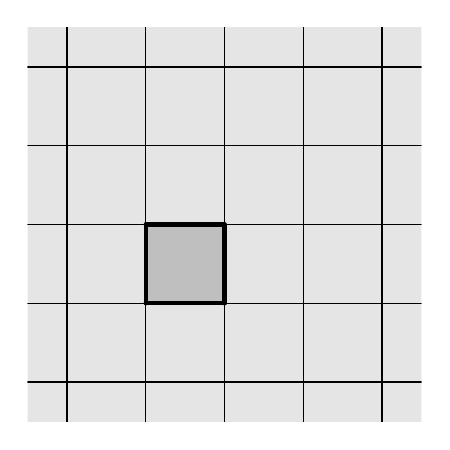
\begin{tikzpicture}[line cap=round,line join=round,>=triangle 45,x=1.0cm,y=1.0cm]
\clip(0.5,0.5) rectangle (5.5,5.5);
\fill[fill=black,fill opacity=0.1] (0,0) -- (1,0) -- (1,1) -- (0,1) -- cycle;
\fill[fill=black,fill opacity=0.1] (1,0) -- (2,0) -- (2,1) -- (1,1) -- cycle;
\fill[fill=black,fill opacity=0.1] (2,0) -- (3,0) -- (3,1) -- (2,1) -- cycle;
\fill[fill=black,fill opacity=0.1] (3,0) -- (4,0) -- (4,1) -- (3,1) -- cycle;
\fill[fill=black,fill opacity=0.1] (4,0) -- (5,0) -- (5,1) -- (4,1) -- cycle;
\fill[fill=black,fill opacity=0.1] (5,0) -- (6,0) -- (6,1) -- (5,1) -- cycle;
\fill[fill=black,fill opacity=0.1] (6,0) -- (7,0) -- (7,1) -- (6,1) -- cycle;
\fill[fill=black,fill opacity=0.1] (7,0) -- (8,0) -- (8,1) -- (7,1) -- cycle;
\fill[fill=black,fill opacity=0.1] (0,1) -- (1,1) -- (1,2) -- (0,2) -- cycle;
\fill[fill=black,fill opacity=0.1] (1,1) -- (2,1) -- (2,2) -- (1,2) -- cycle;
\fill[fill=black,fill opacity=0.1] (2,1) -- (3,1) -- (3,2) -- (2,2) -- cycle;
\fill[fill=black,fill opacity=0.1] (3,1) -- (4,1) -- (4,2) -- (3,2) -- cycle;
\fill[fill=black,fill opacity=0.1] (4,1) -- (5,1) -- (5,2) -- (4,2) -- cycle;
\fill[fill=black,fill opacity=0.1] (5,1) -- (6,1) -- (6,2) -- (5,2) -- cycle;
\fill[fill=black,fill opacity=0.1] (6,1) -- (7,1) -- (7,2) -- (6,2) -- cycle;
\fill[fill=black,fill opacity=0.1] (7,1) -- (8,1) -- (8,2) -- (7,2) -- cycle;
\fill[fill=black,fill opacity=0.1] (0,2) -- (1,2) -- (1,3) -- (0,3) -- cycle;
\fill[fill=black,fill opacity=0.1] (1,2) -- (2,2) -- (2,3) -- (1,3) -- cycle;
\fill[line width=1.6pt,fill=black,fill opacity=0.25] (2,2) -- (3,2) -- (3,3) -- (2,3) -- cycle;
\fill[fill=black,fill opacity=0.1] (3,2) -- (4,2) -- (4,3) -- (3,3) -- cycle;
\fill[fill=black,fill opacity=0.1] (4,2) -- (5,2) -- (5,3) -- (4,3) -- cycle;
\fill[fill=black,fill opacity=0.1] (5,2) -- (6,2) -- (6,3) -- (5,3) -- cycle;
\fill[fill=black,fill opacity=0.1] (6,2) -- (7,2) -- (7,3) -- (6,3) -- cycle;
\fill[fill=black,fill opacity=0.1] (7,2) -- (8,2) -- (8,3) -- (7,3) -- cycle;
\fill[fill=black,fill opacity=0.1] (0,3) -- (1,3) -- (1,4) -- (0,4) -- cycle;
\fill[fill=black,fill opacity=0.1] (1,3) -- (2,3) -- (2,4) -- (1,4) -- cycle;
\fill[fill=black,fill opacity=0.1] (2,3) -- (3,3) -- (3,4) -- (2,4) -- cycle;
\fill[fill=black,fill opacity=0.1] (3,3) -- (4,3) -- (4,4) -- (3,4) -- cycle;
\fill[fill=black,fill opacity=0.1] (4,3) -- (5,3) -- (5,4) -- (4,4) -- cycle;
\fill[fill=black,fill opacity=0.1] (5,3) -- (6,3) -- (6,4) -- (5,4) -- cycle;
\fill[fill=black,fill opacity=0.1] (6,3) -- (7,3) -- (7,4) -- (6,4) -- cycle;
\fill[fill=black,fill opacity=0.1] (7,3) -- (8,3) -- (8,4) -- (7,4) -- cycle;
\fill[fill=black,fill opacity=0.1] (0,4) -- (1,4) -- (1,5) -- (0,5) -- cycle;
\fill[fill=black,fill opacity=0.1] (1,4) -- (2,4) -- (2,5) -- (1,5) -- cycle;
\fill[fill=black,fill opacity=0.1] (2,4) -- (3,4) -- (3,5) -- (2,5) -- cycle;
\fill[fill=black,fill opacity=0.1] (3,4) -- (4,4) -- (4,5) -- (3,5) -- cycle;
\fill[fill=black,fill opacity=0.1] (4,4) -- (5,4) -- (5,5) -- (4,5) -- cycle;
\fill[fill=black,fill opacity=0.1] (5,4) -- (6,4) -- (6,5) -- (5,5) -- cycle;
\fill[fill=black,fill opacity=0.1] (6,4) -- (7,4) -- (7,5) -- (6,5) -- cycle;
\fill[fill=black,fill opacity=0.1] (7,4) -- (8,4) -- (8,5) -- (7,5) -- cycle;
\fill[fill=black,fill opacity=0.1] (0,5) -- (1,5) -- (1,6) -- (0,6) -- cycle;
\fill[fill=black,fill opacity=0.1] (1,5) -- (2,5) -- (2,6) -- (1,6) -- cycle;
\fill[fill=black,fill opacity=0.1] (2,5) -- (3,5) -- (3,6) -- (2,6) -- cycle;
\fill[fill=black,fill opacity=0.1] (3,5) -- (4,5) -- (4,6) -- (3,6) -- cycle;
\fill[fill=black,fill opacity=0.1] (4,5) -- (5,5) -- (5,6) -- (4,6) -- cycle;
\fill[fill=black,fill opacity=0.1] (5,5) -- (6,5) -- (6,6) -- (5,6) -- cycle;
\fill[fill=black,fill opacity=0.1] (6,5) -- (7,5) -- (7,6) -- (6,6) -- cycle;
\fill[fill=black,fill opacity=0.1] (7,5) -- (8,5) -- (8,6) -- (7,6) -- cycle;
\fill[fill=black,fill opacity=0.1] (0,6) -- (1,6) -- (1,7) -- (0,7) -- cycle;
\fill[fill=black,fill opacity=0.1] (1,6) -- (2,6) -- (2,7) -- (1,7) -- cycle;
\fill[fill=black,fill opacity=0.1] (2,6) -- (3,6) -- (3,7) -- (2,7) -- cycle;
\fill[fill=black,fill opacity=0.1] (3,6) -- (4,6) -- (4,7) -- (3,7) -- cycle;
\fill[fill=black,fill opacity=0.1] (4,6) -- (5,6) -- (5,7) -- (4,7) -- cycle;
\fill[fill=black,fill opacity=0.1] (5,6) -- (6,6) -- (6,7) -- (5,7) -- cycle;
\fill[fill=black,fill opacity=0.1] (6,6) -- (7,6) -- (7,7) -- (6,7) -- cycle;
\fill[fill=black,fill opacity=0.1] (7,6) -- (8,6) -- (8,7) -- (7,7) -- cycle;
\fill[fill=black,fill opacity=0.1] (0,7) -- (1,7) -- (1,8) -- (0,8) -- cycle;
\fill[fill=black,fill opacity=0.1] (1,7) -- (2,7) -- (2,8) -- (1,8) -- cycle;
\fill[fill=black,fill opacity=0.1] (2,7) -- (3,7) -- (3,8) -- (2,8) -- cycle;
\fill[fill=black,fill opacity=0.1] (3,7) -- (4,7) -- (4,8) -- (3,8) -- cycle;
\fill[fill=black,fill opacity=0.1] (4,7) -- (5,7) -- (5,8) -- (4,8) -- cycle;
\fill[fill=black,fill opacity=0.1] (5,7) -- (6,7) -- (6,8) -- (5,8) -- cycle;
\fill[fill=black,fill opacity=0.1] (6,7) -- (7,7) -- (7,8) -- (6,8) -- cycle;
\fill[fill=black,fill opacity=0.1] (7,7) -- (8,7) -- (8,8) -- (7,8) -- cycle;
\draw (0,0)-- (1,0);
\draw (1,0)-- (1,1);
\draw (1,1)-- (0,1);
\draw (0,1)-- (0,0);
\draw (1,0)-- (2,0);
\draw (2,0)-- (2,1);
\draw (2,1)-- (1,1);
\draw (1,1)-- (1,0);
\draw (2,0)-- (3,0);
\draw (3,0)-- (3,1);
\draw (3,1)-- (2,1);
\draw (2,1)-- (2,0);
\draw (3,0)-- (4,0);
\draw (4,0)-- (4,1);
\draw (4,1)-- (3,1);
\draw (3,1)-- (3,0);
\draw (4,0)-- (5,0);
\draw (5,0)-- (5,1);
\draw (5,1)-- (4,1);
\draw (4,1)-- (4,0);
\draw (5,0)-- (6,0);
\draw (6,0)-- (6,1);
\draw (6,1)-- (5,1);
\draw (5,1)-- (5,0);
\draw (6,0)-- (7,0);
\draw (7,0)-- (7,1);
\draw (7,1)-- (6,1);
\draw (6,1)-- (6,0);
\draw (7,0)-- (8,0);
\draw (8,0)-- (8,1);
\draw (8,1)-- (7,1);
\draw (7,1)-- (7,0);
\draw (0,1)-- (1,1);
\draw (1,1)-- (1,2);
\draw (1,2)-- (0,2);
\draw (0,2)-- (0,1);
\draw (1,1)-- (2,1);
\draw (2,1)-- (2,2);
\draw (2,2)-- (1,2);
\draw (1,2)-- (1,1);
\draw (2,1)-- (3,1);
\draw (3,1)-- (3,2);
\draw (3,2)-- (2,2);
\draw (2,2)-- (2,1);
\draw (3,1)-- (4,1);
\draw (4,1)-- (4,2);
\draw (4,2)-- (3,2);
\draw (3,2)-- (3,1);
\draw (4,1)-- (5,1);
\draw (5,1)-- (5,2);
\draw (5,2)-- (4,2);
\draw (4,2)-- (4,1);
\draw (5,1)-- (6,1);
\draw (6,1)-- (6,2);
\draw (6,2)-- (5,2);
\draw (5,2)-- (5,1);
\draw (6,1)-- (7,1);
\draw (7,1)-- (7,2);
\draw (7,2)-- (6,2);
\draw (6,2)-- (6,1);
\draw (7,1)-- (8,1);
\draw (8,1)-- (8,2);
\draw (8,2)-- (7,2);
\draw (7,2)-- (7,1);
\draw (0,2)-- (1,2);
\draw (1,2)-- (1,3);
\draw (1,3)-- (0,3);
\draw (0,3)-- (0,2);
\draw (1,2)-- (2,2);
\draw (2,2)-- (2,3);
\draw (2,3)-- (1,3);
\draw (1,3)-- (1,2);
\draw [line width=1.6pt] (2,2)-- (3,2);
\draw [line width=1.6pt] (3,2)-- (3,3);
\draw [line width=1.6pt] (3,3)-- (2,3);
\draw [line width=1.6pt] (2,3)-- (2,2);
\draw (3,2)-- (4,2);
\draw (4,2)-- (4,3);
\draw (4,3)-- (3,3);
\draw (3,3)-- (3,2);
\draw (4,2)-- (5,2);
\draw (5,2)-- (5,3);
\draw (5,3)-- (4,3);
\draw (4,3)-- (4,2);
\draw (5,2)-- (6,2);
\draw (6,2)-- (6,3);
\draw (6,3)-- (5,3);
\draw (5,3)-- (5,2);
\draw (6,2)-- (7,2);
\draw (7,2)-- (7,3);
\draw (7,3)-- (6,3);
\draw (6,3)-- (6,2);
\draw (7,2)-- (8,2);
\draw (8,2)-- (8,3);
\draw (8,3)-- (7,3);
\draw (7,3)-- (7,2);
\draw (0,3)-- (1,3);
\draw (1,3)-- (1,4);
\draw (1,4)-- (0,4);
\draw (0,4)-- (0,3);
\draw (1,3)-- (2,3);
\draw (2,3)-- (2,4);
\draw (2,4)-- (1,4);
\draw (1,4)-- (1,3);
\draw (2,3)-- (3,3);
\draw (3,3)-- (3,4);
\draw (3,4)-- (2,4);
\draw (2,4)-- (2,3);
\draw (3,3)-- (4,3);
\draw (4,3)-- (4,4);
\draw (4,4)-- (3,4);
\draw (3,4)-- (3,3);
\draw (4,3)-- (5,3);
\draw (5,3)-- (5,4);
\draw (5,4)-- (4,4);
\draw (4,4)-- (4,3);
\draw (5,3)-- (6,3);
\draw (6,3)-- (6,4);
\draw (6,4)-- (5,4);
\draw (5,4)-- (5,3);
\draw (6,3)-- (7,3);
\draw (7,3)-- (7,4);
\draw (7,4)-- (6,4);
\draw (6,4)-- (6,3);
\draw (7,3)-- (8,3);
\draw (8,3)-- (8,4);
\draw (8,4)-- (7,4);
\draw (7,4)-- (7,3);
\draw (0,4)-- (1,4);
\draw (1,4)-- (1,5);
\draw (1,5)-- (0,5);
\draw (0,5)-- (0,4);
\draw (1,4)-- (2,4);
\draw (2,4)-- (2,5);
\draw (2,5)-- (1,5);
\draw (1,5)-- (1,4);
\draw (2,4)-- (3,4);
\draw (3,4)-- (3,5);
\draw (3,5)-- (2,5);
\draw (2,5)-- (2,4);
\draw (3,4)-- (4,4);
\draw (4,4)-- (4,5);
\draw (4,5)-- (3,5);
\draw (3,5)-- (3,4);
\draw (4,4)-- (5,4);
\draw (5,4)-- (5,5);
\draw (5,5)-- (4,5);
\draw (4,5)-- (4,4);
\draw (5,4)-- (6,4);
\draw (6,4)-- (6,5);
\draw (6,5)-- (5,5);
\draw (5,5)-- (5,4);
\draw (6,4)-- (7,4);
\draw (7,4)-- (7,5);
\draw (7,5)-- (6,5);
\draw (6,5)-- (6,4);
\draw (7,4)-- (8,4);
\draw (8,4)-- (8,5);
\draw (8,5)-- (7,5);
\draw (7,5)-- (7,4);
\draw (0,5)-- (1,5);
\draw (1,5)-- (1,6);
\draw (1,6)-- (0,6);
\draw (0,6)-- (0,5);
\draw (1,5)-- (2,5);
\draw (2,5)-- (2,6);
\draw (2,6)-- (1,6);
\draw (1,6)-- (1,5);
\draw (2,5)-- (3,5);
\draw (3,5)-- (3,6);
\draw (3,6)-- (2,6);
\draw (2,6)-- (2,5);
\draw (3,5)-- (4,5);
\draw (4,5)-- (4,6);
\draw (4,6)-- (3,6);
\draw (3,6)-- (3,5);
\draw (4,5)-- (5,5);
\draw (5,5)-- (5,6);
\draw (5,6)-- (4,6);
\draw (4,6)-- (4,5);
\draw (5,5)-- (6,5);
\draw (6,5)-- (6,6);
\draw (6,6)-- (5,6);
\draw (5,6)-- (5,5);
\draw (6,5)-- (7,5);
\draw (7,5)-- (7,6);
\draw (7,6)-- (6,6);
\draw (6,6)-- (6,5);
\draw (7,5)-- (8,5);
\draw (8,5)-- (8,6);
\draw (8,6)-- (7,6);
\draw (7,6)-- (7,5);
\draw (0,6)-- (1,6);
\draw (1,6)-- (1,7);
\draw (1,7)-- (0,7);
\draw (0,7)-- (0,6);
\draw (1,6)-- (2,6);
\draw (2,6)-- (2,7);
\draw (2,7)-- (1,7);
\draw (1,7)-- (1,6);
\draw (2,6)-- (3,6);
\draw (3,6)-- (3,7);
\draw (3,7)-- (2,7);
\draw (2,7)-- (2,6);
\draw (3,6)-- (4,6);
\draw (4,6)-- (4,7);
\draw (4,7)-- (3,7);
\draw (3,7)-- (3,6);
\draw (4,6)-- (5,6);
\draw (5,6)-- (5,7);
\draw (5,7)-- (4,7);
\draw (4,7)-- (4,6);
\draw (5,6)-- (6,6);
\draw (6,6)-- (6,7);
\draw (6,7)-- (5,7);
\draw (5,7)-- (5,6);
\draw (6,6)-- (7,6);
\draw (7,6)-- (7,7);
\draw (7,7)-- (6,7);
\draw (6,7)-- (6,6);
\draw (7,6)-- (8,6);
\draw (8,6)-- (8,7);
\draw (8,7)-- (7,7);
\draw (7,7)-- (7,6);
\draw (0,7)-- (1,7);
\draw (1,7)-- (1,8);
\draw (1,8)-- (0,8);
\draw (0,8)-- (0,7);
\draw (1,7)-- (2,7);
\draw (2,7)-- (2,8);
\draw (2,8)-- (1,8);
\draw (1,8)-- (1,7);
\draw (2,7)-- (3,7);
\draw (3,7)-- (3,8);
\draw (3,8)-- (2,8);
\draw (2,8)-- (2,7);
\draw (3,7)-- (4,7);
\draw (4,7)-- (4,8);
\draw (4,8)-- (3,8);
\draw (3,8)-- (3,7);
\draw (4,7)-- (5,7);
\draw (5,7)-- (5,8);
\draw (5,8)-- (4,8);
\draw (4,8)-- (4,7);
\draw (5,7)-- (6,7);
\draw (6,7)-- (6,8);
\draw (6,8)-- (5,8);
\draw (5,8)-- (5,7);
\draw (6,7)-- (7,7);
\draw (7,7)-- (7,8);
\draw (7,8)-- (6,8);
\draw (6,8)-- (6,7);
\draw (7,7)-- (8,7);
\draw (8,7)-- (8,8);
\draw (8,8)-- (7,8);
\draw (7,8)-- (7,7);
\end{tikzpicture}
}
  \subfloat[Regelmatige zeshoeken]{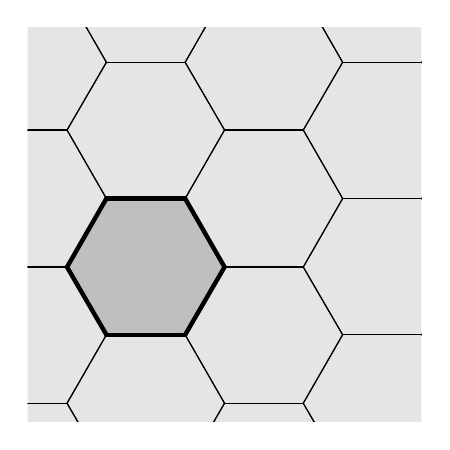
\begin{tikzpicture}[line cap=round,line join=round,>=triangle 45,x=1.0cm,y=1.0cm]
\clip(0.5,1.5) rectangle (5.5,6.5);
\fill[fill=black,fill opacity=0.1] (0,0) -- (1,0) -- (1.5,0.87) -- (1,1.73) -- (0,1.73) -- (-0.5,0.87) -- cycle;
\fill[fill=black,fill opacity=0.1] (1.5,0.87) -- (2.5,0.87) -- (3,1.73) -- (2.5,2.6) -- (1.5,2.6) -- (1,1.73) -- cycle;
\fill[fill=black,fill opacity=0.1] (3,0) -- (4,0) -- (4.5,0.87) -- (4,1.73) -- (3,1.73) -- (2.5,0.87) -- cycle;
\fill[fill=black,fill opacity=0.1] (4.5,0.87) -- (5.5,0.87) -- (6,1.73) -- (5.5,2.6) -- (4.5,2.6) -- (4,1.73) -- cycle;
\fill[fill=black,fill opacity=0.1] (6,0) -- (7,0) -- (7.5,0.87) -- (7,1.73) -- (6,1.73) -- (5.5,0.87) -- cycle;
\fill[fill=black,fill opacity=0.1] (7.5,0.87) -- (8.5,0.87) -- (9,1.73) -- (8.5,2.6) -- (7.5,2.6) -- (7,1.73) -- cycle;
\fill[fill=black,fill opacity=0.1] (9,0) -- (10,0) -- (10.5,0.87) -- (10,1.73) -- (9,1.73) -- (8.5,0.87) -- cycle;
\fill[fill=black,fill opacity=0.1] (10.5,0.87) -- (11.5,0.87) -- (12,1.73) -- (11.5,2.6) -- (10.5,2.6) -- (10,1.73) -- cycle;
\fill[fill=black,fill opacity=0.1] (0,1.73) -- (1,1.73) -- (1.5,2.6) -- (1,3.46) -- (0,3.46) -- (-0.5,2.6) -- cycle;
\fill[line width=1.6pt,fill=black,fill opacity=0.25] (1.5,2.6) -- (2.5,2.6) -- (3,3.46) -- (2.5,4.33) -- (1.5,4.33) -- (1,3.46) -- cycle;
\fill[fill=black,fill opacity=0.1] (3,1.73) -- (4,1.73) -- (4.5,2.6) -- (4,3.46) -- (3,3.46) -- (2.5,2.6) -- cycle;
\fill[fill=black,fill opacity=0.1] (4.5,2.6) -- (5.5,2.6) -- (6,3.46) -- (5.5,4.33) -- (4.5,4.33) -- (4,3.46) -- cycle;
\fill[fill=black,fill opacity=0.1] (6,1.73) -- (7,1.73) -- (7.5,2.6) -- (7,3.46) -- (6,3.46) -- (5.5,2.6) -- cycle;
\fill[fill=black,fill opacity=0.1] (7.5,2.6) -- (8.5,2.6) -- (9,3.46) -- (8.5,4.33) -- (7.5,4.33) -- (7,3.46) -- cycle;
\fill[fill=black,fill opacity=0.1] (9,1.73) -- (10,1.73) -- (10.5,2.6) -- (10,3.46) -- (9,3.46) -- (8.5,2.6) -- cycle;
\fill[fill=black,fill opacity=0.1] (10.5,2.6) -- (11.5,2.6) -- (12,3.46) -- (11.5,4.33) -- (10.5,4.33) -- (10,3.46) -- cycle;
\fill[fill=black,fill opacity=0.1] (0,3.46) -- (1,3.46) -- (1.5,4.33) -- (1,5.2) -- (0,5.2) -- (-0.5,4.33) -- cycle;
\fill[fill=black,fill opacity=0.1] (1.5,4.33) -- (2.5,4.33) -- (3,5.2) -- (2.5,6.06) -- (1.5,6.06) -- (1,5.2) -- cycle;
\fill[fill=black,fill opacity=0.1] (3,3.46) -- (4,3.46) -- (4.5,4.33) -- (4,5.2) -- (3,5.2) -- (2.5,4.33) -- cycle;
\fill[fill=black,fill opacity=0.1] (4.5,4.33) -- (5.5,4.33) -- (6,5.2) -- (5.5,6.06) -- (4.5,6.06) -- (4,5.2) -- cycle;
\fill[fill=black,fill opacity=0.1] (6,3.46) -- (7,3.46) -- (7.5,4.33) -- (7,5.2) -- (6,5.2) -- (5.5,4.33) -- cycle;
\fill[fill=black,fill opacity=0.1] (7.5,4.33) -- (8.5,4.33) -- (9,5.2) -- (8.5,6.06) -- (7.5,6.06) -- (7,5.2) -- cycle;
\fill[fill=black,fill opacity=0.1] (9,3.46) -- (10,3.46) -- (10.5,4.33) -- (10,5.2) -- (9,5.2) -- (8.5,4.33) -- cycle;
\fill[fill=black,fill opacity=0.1] (10.5,4.33) -- (11.5,4.33) -- (12,5.2) -- (11.5,6.06) -- (10.5,6.06) -- (10,5.2) -- cycle;
\fill[fill=black,fill opacity=0.1] (0,5.2) -- (1,5.2) -- (1.5,6.06) -- (1,6.93) -- (0,6.93) -- (-0.5,6.06) -- cycle;
\fill[fill=black,fill opacity=0.1] (1.5,6.06) -- (2.5,6.06) -- (3,6.93) -- (2.5,7.79) -- (1.5,7.79) -- (1,6.93) -- cycle;
\fill[fill=black,fill opacity=0.1] (3,5.2) -- (4,5.2) -- (4.5,6.06) -- (4,6.93) -- (3,6.93) -- (2.5,6.06) -- cycle;
\fill[fill=black,fill opacity=0.1] (4.5,6.06) -- (5.5,6.06) -- (6,6.93) -- (5.5,7.79) -- (4.5,7.79) -- (4,6.93) -- cycle;
\fill[fill=black,fill opacity=0.1] (6,5.2) -- (7,5.2) -- (7.5,6.06) -- (7,6.93) -- (6,6.93) -- (5.5,6.06) -- cycle;
\fill[fill=black,fill opacity=0.1] (7.5,6.06) -- (8.5,6.06) -- (9,6.93) -- (8.5,7.79) -- (7.5,7.79) -- (7,6.93) -- cycle;
\fill[fill=black,fill opacity=0.1] (9,5.2) -- (10,5.2) -- (10.5,6.06) -- (10,6.93) -- (9,6.93) -- (8.5,6.06) -- cycle;
\fill[fill=black,fill opacity=0.1] (10.5,6.06) -- (11.5,6.06) -- (12,6.93) -- (11.5,7.79) -- (10.5,7.79) -- (10,6.93) -- cycle;
\fill[fill=black,fill opacity=0.1] (0,6.93) -- (1,6.93) -- (1.5,7.79) -- (1,8.66) -- (0,8.66) -- (-0.5,7.79) -- cycle;
\fill[fill=black,fill opacity=0.1] (1.5,7.79) -- (2.5,7.79) -- (3,8.66) -- (2.5,9.53) -- (1.5,9.53) -- (1,8.66) -- cycle;
\fill[fill=black,fill opacity=0.1] (3,6.93) -- (4,6.93) -- (4.5,7.79) -- (4,8.66) -- (3,8.66) -- (2.5,7.79) -- cycle;
\fill[fill=black,fill opacity=0.1] (4.5,7.79) -- (5.5,7.79) -- (6,8.66) -- (5.5,9.53) -- (4.5,9.53) -- (4,8.66) -- cycle;
\fill[fill=black,fill opacity=0.1] (6,6.93) -- (7,6.93) -- (7.5,7.79) -- (7,8.66) -- (6,8.66) -- (5.5,7.79) -- cycle;
\fill[fill=black,fill opacity=0.1] (7.5,7.79) -- (8.5,7.79) -- (9,8.66) -- (8.5,9.53) -- (7.5,9.53) -- (7,8.66) -- cycle;
\fill[fill=black,fill opacity=0.1] (9,6.93) -- (10,6.93) -- (10.5,7.79) -- (10,8.66) -- (9,8.66) -- (8.5,7.79) -- cycle;
\fill[fill=black,fill opacity=0.1] (10.5,7.79) -- (11.5,7.79) -- (12,8.66) -- (11.5,9.53) -- (10.5,9.53) -- (10,8.66) -- cycle;
\fill[fill=black,fill opacity=0.1] (0,8.66) -- (1,8.66) -- (1.5,9.53) -- (1,10.39) -- (0,10.39) -- (-0.5,9.53) -- cycle;
\fill[fill=black,fill opacity=0.1] (1.5,9.53) -- (2.5,9.53) -- (3,10.39) -- (2.5,11.26) -- (1.5,11.26) -- (1,10.39) -- cycle;
\fill[fill=black,fill opacity=0.1] (3,8.66) -- (4,8.66) -- (4.5,9.53) -- (4,10.39) -- (3,10.39) -- (2.5,9.53) -- cycle;
\fill[fill=black,fill opacity=0.1] (4.5,9.53) -- (5.5,9.53) -- (6,10.39) -- (5.5,11.26) -- (4.5,11.26) -- (4,10.39) -- cycle;
\fill[fill=black,fill opacity=0.1] (6,8.66) -- (7,8.66) -- (7.5,9.53) -- (7,10.39) -- (6,10.39) -- (5.5,9.53) -- cycle;
\fill[fill=black,fill opacity=0.1] (7.5,9.53) -- (8.5,9.53) -- (9,10.39) -- (8.5,11.26) -- (7.5,11.26) -- (7,10.39) -- cycle;
\fill[fill=black,fill opacity=0.1] (9,8.66) -- (10,8.66) -- (10.5,9.53) -- (10,10.39) -- (9,10.39) -- (8.5,9.53) -- cycle;
\fill[fill=black,fill opacity=0.1] (10.5,9.53) -- (11.5,9.53) -- (12,10.39) -- (11.5,11.26) -- (10.5,11.26) -- (10,10.39) -- cycle;
\fill[fill=black,fill opacity=0.1] (0,10.39) -- (1,10.39) -- (1.5,11.26) -- (1,12.12) -- (0,12.12) -- (-0.5,11.26) -- cycle;
\fill[fill=black,fill opacity=0.1] (1.5,11.26) -- (2.5,11.26) -- (3,12.12) -- (2.5,12.99) -- (1.5,12.99) -- (1,12.12) -- cycle;
\fill[fill=black,fill opacity=0.1] (3,10.39) -- (4,10.39) -- (4.5,11.26) -- (4,12.12) -- (3,12.12) -- (2.5,11.26) -- cycle;
\fill[fill=black,fill opacity=0.1] (4.5,11.26) -- (5.5,11.26) -- (6,12.12) -- (5.5,12.99) -- (4.5,12.99) -- (4,12.12) -- cycle;
\fill[fill=black,fill opacity=0.1] (6,10.39) -- (7,10.39) -- (7.5,11.26) -- (7,12.12) -- (6,12.12) -- (5.5,11.26) -- cycle;
\fill[fill=black,fill opacity=0.1] (7.5,11.26) -- (8.5,11.26) -- (9,12.12) -- (8.5,12.99) -- (7.5,12.99) -- (7,12.12) -- cycle;
\fill[fill=black,fill opacity=0.1] (9,10.39) -- (10,10.39) -- (10.5,11.26) -- (10,12.12) -- (9,12.12) -- (8.5,11.26) -- cycle;
\fill[fill=black,fill opacity=0.1] (10.5,11.26) -- (11.5,11.26) -- (12,12.12) -- (11.5,12.99) -- (10.5,12.99) -- (10,12.12) -- cycle;
\fill[fill=black,fill opacity=0.1] (0,12.12) -- (1,12.12) -- (1.5,12.99) -- (1,13.86) -- (0,13.86) -- (-0.5,12.99) -- cycle;
\fill[fill=black,fill opacity=0.1] (1.5,12.99) -- (2.5,12.99) -- (3,13.86) -- (2.5,14.72) -- (1.5,14.72) -- (1,13.86) -- cycle;
\fill[fill=black,fill opacity=0.1] (3,12.12) -- (4,12.12) -- (4.5,12.99) -- (4,13.86) -- (3,13.86) -- (2.5,12.99) -- cycle;
\fill[fill=black,fill opacity=0.1] (4.5,12.99) -- (5.5,12.99) -- (6,13.86) -- (5.5,14.72) -- (4.5,14.72) -- (4,13.86) -- cycle;
\fill[fill=black,fill opacity=0.1] (6,12.12) -- (7,12.12) -- (7.5,12.99) -- (7,13.86) -- (6,13.86) -- (5.5,12.99) -- cycle;
\fill[fill=black,fill opacity=0.1] (7.5,12.99) -- (8.5,12.99) -- (9,13.86) -- (8.5,14.72) -- (7.5,14.72) -- (7,13.86) -- cycle;
\fill[fill=black,fill opacity=0.1] (9,12.12) -- (10,12.12) -- (10.5,12.99) -- (10,13.86) -- (9,13.86) -- (8.5,12.99) -- cycle;
\fill[fill=black,fill opacity=0.1] (10.5,12.99) -- (11.5,12.99) -- (12,13.86) -- (11.5,14.72) -- (10.5,14.72) -- (10,13.86) -- cycle;
\draw (0,0)-- (1,0);
\draw (1,0)-- (1.5,0.87);
\draw (1.5,0.87)-- (1,1.73);
\draw (1,1.73)-- (0,1.73);
\draw (0,1.73)-- (-0.5,0.87);
\draw (-0.5,0.87)-- (0,0);
\draw (1.5,0.87)-- (2.5,0.87);
\draw (2.5,0.87)-- (3,1.73);
\draw (3,1.73)-- (2.5,2.6);
\draw (2.5,2.6)-- (1.5,2.6);
\draw (1.5,2.6)-- (1,1.73);
\draw (1,1.73)-- (1.5,0.87);
\draw (3,0)-- (4,0);
\draw (4,0)-- (4.5,0.87);
\draw (4.5,0.87)-- (4,1.73);
\draw (4,1.73)-- (3,1.73);
\draw (3,1.73)-- (2.5,0.87);
\draw (2.5,0.87)-- (3,0);
\draw (4.5,0.87)-- (5.5,0.87);
\draw (5.5,0.87)-- (6,1.73);
\draw (6,1.73)-- (5.5,2.6);
\draw (5.5,2.6)-- (4.5,2.6);
\draw (4.5,2.6)-- (4,1.73);
\draw (4,1.73)-- (4.5,0.87);
\draw (6,0)-- (7,0);
\draw (7,0)-- (7.5,0.87);
\draw (7.5,0.87)-- (7,1.73);
\draw (7,1.73)-- (6,1.73);
\draw (6,1.73)-- (5.5,0.87);
\draw (5.5,0.87)-- (6,0);
\draw (7.5,0.87)-- (8.5,0.87);
\draw (8.5,0.87)-- (9,1.73);
\draw (9,1.73)-- (8.5,2.6);
\draw (8.5,2.6)-- (7.5,2.6);
\draw (7.5,2.6)-- (7,1.73);
\draw (7,1.73)-- (7.5,0.87);
\draw (9,0)-- (10,0);
\draw (10,0)-- (10.5,0.87);
\draw (10.5,0.87)-- (10,1.73);
\draw (10,1.73)-- (9,1.73);
\draw (9,1.73)-- (8.5,0.87);
\draw (8.5,0.87)-- (9,0);
\draw (10.5,0.87)-- (11.5,0.87);
\draw (11.5,0.87)-- (12,1.73);
\draw (12,1.73)-- (11.5,2.6);
\draw (11.5,2.6)-- (10.5,2.6);
\draw (10.5,2.6)-- (10,1.73);
\draw (10,1.73)-- (10.5,0.87);
\draw (0,1.73)-- (1,1.73);
\draw (1,1.73)-- (1.5,2.6);
\draw (1.5,2.6)-- (1,3.46);
\draw (1,3.46)-- (0,3.46);
\draw (0,3.46)-- (-0.5,2.6);
\draw (-0.5,2.6)-- (0,1.73);
\draw [line width=1.6pt] (1.5,2.6)-- (2.5,2.6);
\draw [line width=1.6pt] (2.5,2.6)-- (3,3.46);
\draw [line width=1.6pt] (3,3.46)-- (2.5,4.33);
\draw [line width=1.6pt] (2.5,4.33)-- (1.5,4.33);
\draw [line width=1.6pt] (1.5,4.33)-- (1,3.46);
\draw [line width=1.6pt] (1,3.46)-- (1.5,2.6);
\draw (3,1.73)-- (4,1.73);
\draw (4,1.73)-- (4.5,2.6);
\draw (4.5,2.6)-- (4,3.46);
\draw (4,3.46)-- (3,3.46);
\draw (3,3.46)-- (2.5,2.6);
\draw (2.5,2.6)-- (3,1.73);
\draw (4.5,2.6)-- (5.5,2.6);
\draw (5.5,2.6)-- (6,3.46);
\draw (6,3.46)-- (5.5,4.33);
\draw (5.5,4.33)-- (4.5,4.33);
\draw (4.5,4.33)-- (4,3.46);
\draw (4,3.46)-- (4.5,2.6);
\draw (6,1.73)-- (7,1.73);
\draw (7,1.73)-- (7.5,2.6);
\draw (7.5,2.6)-- (7,3.46);
\draw (7,3.46)-- (6,3.46);
\draw (6,3.46)-- (5.5,2.6);
\draw (5.5,2.6)-- (6,1.73);
\draw (7.5,2.6)-- (8.5,2.6);
\draw (8.5,2.6)-- (9,3.46);
\draw (9,3.46)-- (8.5,4.33);
\draw (8.5,4.33)-- (7.5,4.33);
\draw (7.5,4.33)-- (7,3.46);
\draw (7,3.46)-- (7.5,2.6);
\draw (9,1.73)-- (10,1.73);
\draw (10,1.73)-- (10.5,2.6);
\draw (10.5,2.6)-- (10,3.46);
\draw (10,3.46)-- (9,3.46);
\draw (9,3.46)-- (8.5,2.6);
\draw (8.5,2.6)-- (9,1.73);
\draw (10.5,2.6)-- (11.5,2.6);
\draw (11.5,2.6)-- (12,3.46);
\draw (12,3.46)-- (11.5,4.33);
\draw (11.5,4.33)-- (10.5,4.33);
\draw (10.5,4.33)-- (10,3.46);
\draw (10,3.46)-- (10.5,2.6);
\draw (0,3.46)-- (1,3.46);
\draw (1,3.46)-- (1.5,4.33);
\draw (1.5,4.33)-- (1,5.2);
\draw (1,5.2)-- (0,5.2);
\draw (0,5.2)-- (-0.5,4.33);
\draw (-0.5,4.33)-- (0,3.46);
\draw (1.5,4.33)-- (2.5,4.33);
\draw (2.5,4.33)-- (3,5.2);
\draw (3,5.2)-- (2.5,6.06);
\draw (2.5,6.06)-- (1.5,6.06);
\draw (1.5,6.06)-- (1,5.2);
\draw (1,5.2)-- (1.5,4.33);
\draw (3,3.46)-- (4,3.46);
\draw (4,3.46)-- (4.5,4.33);
\draw (4.5,4.33)-- (4,5.2);
\draw (4,5.2)-- (3,5.2);
\draw (3,5.2)-- (2.5,4.33);
\draw (2.5,4.33)-- (3,3.46);
\draw (4.5,4.33)-- (5.5,4.33);
\draw (5.5,4.33)-- (6,5.2);
\draw (6,5.2)-- (5.5,6.06);
\draw (5.5,6.06)-- (4.5,6.06);
\draw (4.5,6.06)-- (4,5.2);
\draw (4,5.2)-- (4.5,4.33);
\draw (6,3.46)-- (7,3.46);
\draw (7,3.46)-- (7.5,4.33);
\draw (7.5,4.33)-- (7,5.2);
\draw (7,5.2)-- (6,5.2);
\draw (6,5.2)-- (5.5,4.33);
\draw (5.5,4.33)-- (6,3.46);
\draw (7.5,4.33)-- (8.5,4.33);
\draw (8.5,4.33)-- (9,5.2);
\draw (9,5.2)-- (8.5,6.06);
\draw (8.5,6.06)-- (7.5,6.06);
\draw (7.5,6.06)-- (7,5.2);
\draw (7,5.2)-- (7.5,4.33);
\draw (9,3.46)-- (10,3.46);
\draw (10,3.46)-- (10.5,4.33);
\draw (10.5,4.33)-- (10,5.2);
\draw (10,5.2)-- (9,5.2);
\draw (9,5.2)-- (8.5,4.33);
\draw (8.5,4.33)-- (9,3.46);
\draw (10.5,4.33)-- (11.5,4.33);
\draw (11.5,4.33)-- (12,5.2);
\draw (12,5.2)-- (11.5,6.06);
\draw (11.5,6.06)-- (10.5,6.06);
\draw (10.5,6.06)-- (10,5.2);
\draw (10,5.2)-- (10.5,4.33);
\draw (0,5.2)-- (1,5.2);
\draw (1,5.2)-- (1.5,6.06);
\draw (1.5,6.06)-- (1,6.93);
\draw (1,6.93)-- (0,6.93);
\draw (0,6.93)-- (-0.5,6.06);
\draw (-0.5,6.06)-- (0,5.2);
\draw (1.5,6.06)-- (2.5,6.06);
\draw (2.5,6.06)-- (3,6.93);
\draw (3,6.93)-- (2.5,7.79);
\draw (2.5,7.79)-- (1.5,7.79);
\draw (1.5,7.79)-- (1,6.93);
\draw (1,6.93)-- (1.5,6.06);
\draw (3,5.2)-- (4,5.2);
\draw (4,5.2)-- (4.5,6.06);
\draw (4.5,6.06)-- (4,6.93);
\draw (4,6.93)-- (3,6.93);
\draw (3,6.93)-- (2.5,6.06);
\draw (2.5,6.06)-- (3,5.2);
\draw (4.5,6.06)-- (5.5,6.06);
\draw (5.5,6.06)-- (6,6.93);
\draw (6,6.93)-- (5.5,7.79);
\draw (5.5,7.79)-- (4.5,7.79);
\draw (4.5,7.79)-- (4,6.93);
\draw (4,6.93)-- (4.5,6.06);
\draw (6,5.2)-- (7,5.2);
\draw (7,5.2)-- (7.5,6.06);
\draw (7.5,6.06)-- (7,6.93);
\draw (7,6.93)-- (6,6.93);
\draw (6,6.93)-- (5.5,6.06);
\draw (5.5,6.06)-- (6,5.2);
\draw (7.5,6.06)-- (8.5,6.06);
\draw (8.5,6.06)-- (9,6.93);
\draw (9,6.93)-- (8.5,7.79);
\draw (8.5,7.79)-- (7.5,7.79);
\draw (7.5,7.79)-- (7,6.93);
\draw (7,6.93)-- (7.5,6.06);
\draw (9,5.2)-- (10,5.2);
\draw (10,5.2)-- (10.5,6.06);
\draw (10.5,6.06)-- (10,6.93);
\draw (10,6.93)-- (9,6.93);
\draw (9,6.93)-- (8.5,6.06);
\draw (8.5,6.06)-- (9,5.2);
\draw (10.5,6.06)-- (11.5,6.06);
\draw (11.5,6.06)-- (12,6.93);
\draw (12,6.93)-- (11.5,7.79);
\draw (11.5,7.79)-- (10.5,7.79);
\draw (10.5,7.79)-- (10,6.93);
\draw (10,6.93)-- (10.5,6.06);
\draw (0,6.93)-- (1,6.93);
\draw (1,6.93)-- (1.5,7.79);
\draw (1.5,7.79)-- (1,8.66);
\draw (1,8.66)-- (0,8.66);
\draw (0,8.66)-- (-0.5,7.79);
\draw (-0.5,7.79)-- (0,6.93);
\draw (1.5,7.79)-- (2.5,7.79);
\draw (2.5,7.79)-- (3,8.66);
\draw (3,8.66)-- (2.5,9.53);
\draw (2.5,9.53)-- (1.5,9.53);
\draw (1.5,9.53)-- (1,8.66);
\draw (1,8.66)-- (1.5,7.79);
\draw (3,6.93)-- (4,6.93);
\draw (4,6.93)-- (4.5,7.79);
\draw (4.5,7.79)-- (4,8.66);
\draw (4,8.66)-- (3,8.66);
\draw (3,8.66)-- (2.5,7.79);
\draw (2.5,7.79)-- (3,6.93);
\draw (4.5,7.79)-- (5.5,7.79);
\draw (5.5,7.79)-- (6,8.66);
\draw (6,8.66)-- (5.5,9.53);
\draw (5.5,9.53)-- (4.5,9.53);
\draw (4.5,9.53)-- (4,8.66);
\draw (4,8.66)-- (4.5,7.79);
\draw (6,6.93)-- (7,6.93);
\draw (7,6.93)-- (7.5,7.79);
\draw (7.5,7.79)-- (7,8.66);
\draw (7,8.66)-- (6,8.66);
\draw (6,8.66)-- (5.5,7.79);
\draw (5.5,7.79)-- (6,6.93);
\draw (7.5,7.79)-- (8.5,7.79);
\draw (8.5,7.79)-- (9,8.66);
\draw (9,8.66)-- (8.5,9.53);
\draw (8.5,9.53)-- (7.5,9.53);
\draw (7.5,9.53)-- (7,8.66);
\draw (7,8.66)-- (7.5,7.79);
\draw (9,6.93)-- (10,6.93);
\draw (10,6.93)-- (10.5,7.79);
\draw (10.5,7.79)-- (10,8.66);
\draw (10,8.66)-- (9,8.66);
\draw (9,8.66)-- (8.5,7.79);
\draw (8.5,7.79)-- (9,6.93);
\draw (10.5,7.79)-- (11.5,7.79);
\draw (11.5,7.79)-- (12,8.66);
\draw (12,8.66)-- (11.5,9.53);
\draw (11.5,9.53)-- (10.5,9.53);
\draw (10.5,9.53)-- (10,8.66);
\draw (10,8.66)-- (10.5,7.79);
\draw (0,8.66)-- (1,8.66);
\draw (1,8.66)-- (1.5,9.53);
\draw (1.5,9.53)-- (1,10.39);
\draw (1,10.39)-- (0,10.39);
\draw (0,10.39)-- (-0.5,9.53);
\draw (-0.5,9.53)-- (0,8.66);
\draw (1.5,9.53)-- (2.5,9.53);
\draw (2.5,9.53)-- (3,10.39);
\draw (3,10.39)-- (2.5,11.26);
\draw (2.5,11.26)-- (1.5,11.26);
\draw (1.5,11.26)-- (1,10.39);
\draw (1,10.39)-- (1.5,9.53);
\draw (3,8.66)-- (4,8.66);
\draw (4,8.66)-- (4.5,9.53);
\draw (4.5,9.53)-- (4,10.39);
\draw (4,10.39)-- (3,10.39);
\draw (3,10.39)-- (2.5,9.53);
\draw (2.5,9.53)-- (3,8.66);
\draw (4.5,9.53)-- (5.5,9.53);
\draw (5.5,9.53)-- (6,10.39);
\draw (6,10.39)-- (5.5,11.26);
\draw (5.5,11.26)-- (4.5,11.26);
\draw (4.5,11.26)-- (4,10.39);
\draw (4,10.39)-- (4.5,9.53);
\draw (6,8.66)-- (7,8.66);
\draw (7,8.66)-- (7.5,9.53);
\draw (7.5,9.53)-- (7,10.39);
\draw (7,10.39)-- (6,10.39);
\draw (6,10.39)-- (5.5,9.53);
\draw (5.5,9.53)-- (6,8.66);
\draw (7.5,9.53)-- (8.5,9.53);
\draw (8.5,9.53)-- (9,10.39);
\draw (9,10.39)-- (8.5,11.26);
\draw (8.5,11.26)-- (7.5,11.26);
\draw (7.5,11.26)-- (7,10.39);
\draw (7,10.39)-- (7.5,9.53);
\draw (9,8.66)-- (10,8.66);
\draw (10,8.66)-- (10.5,9.53);
\draw (10.5,9.53)-- (10,10.39);
\draw (10,10.39)-- (9,10.39);
\draw (9,10.39)-- (8.5,9.53);
\draw (8.5,9.53)-- (9,8.66);
\draw (10.5,9.53)-- (11.5,9.53);
\draw (11.5,9.53)-- (12,10.39);
\draw (12,10.39)-- (11.5,11.26);
\draw (11.5,11.26)-- (10.5,11.26);
\draw (10.5,11.26)-- (10,10.39);
\draw (10,10.39)-- (10.5,9.53);
\draw (0,10.39)-- (1,10.39);
\draw (1,10.39)-- (1.5,11.26);
\draw (1.5,11.26)-- (1,12.12);
\draw (1,12.12)-- (0,12.12);
\draw (0,12.12)-- (-0.5,11.26);
\draw (-0.5,11.26)-- (0,10.39);
\draw (1.5,11.26)-- (2.5,11.26);
\draw (2.5,11.26)-- (3,12.12);
\draw (3,12.12)-- (2.5,12.99);
\draw (2.5,12.99)-- (1.5,12.99);
\draw (1.5,12.99)-- (1,12.12);
\draw (1,12.12)-- (1.5,11.26);
\draw (3,10.39)-- (4,10.39);
\draw (4,10.39)-- (4.5,11.26);
\draw (4.5,11.26)-- (4,12.12);
\draw (4,12.12)-- (3,12.12);
\draw (3,12.12)-- (2.5,11.26);
\draw (2.5,11.26)-- (3,10.39);
\draw (4.5,11.26)-- (5.5,11.26);
\draw (5.5,11.26)-- (6,12.12);
\draw (6,12.12)-- (5.5,12.99);
\draw (5.5,12.99)-- (4.5,12.99);
\draw (4.5,12.99)-- (4,12.12);
\draw (4,12.12)-- (4.5,11.26);
\draw (6,10.39)-- (7,10.39);
\draw (7,10.39)-- (7.5,11.26);
\draw (7.5,11.26)-- (7,12.12);
\draw (7,12.12)-- (6,12.12);
\draw (6,12.12)-- (5.5,11.26);
\draw (5.5,11.26)-- (6,10.39);
\draw (7.5,11.26)-- (8.5,11.26);
\draw (8.5,11.26)-- (9,12.12);
\draw (9,12.12)-- (8.5,12.99);
\draw (8.5,12.99)-- (7.5,12.99);
\draw (7.5,12.99)-- (7,12.12);
\draw (7,12.12)-- (7.5,11.26);
\draw (9,10.39)-- (10,10.39);
\draw (10,10.39)-- (10.5,11.26);
\draw (10.5,11.26)-- (10,12.12);
\draw (10,12.12)-- (9,12.12);
\draw (9,12.12)-- (8.5,11.26);
\draw (8.5,11.26)-- (9,10.39);
\draw (10.5,11.26)-- (11.5,11.26);
\draw (11.5,11.26)-- (12,12.12);
\draw (12,12.12)-- (11.5,12.99);
\draw (11.5,12.99)-- (10.5,12.99);
\draw (10.5,12.99)-- (10,12.12);
\draw (10,12.12)-- (10.5,11.26);
\draw (0,12.12)-- (1,12.12);
\draw (1,12.12)-- (1.5,12.99);
\draw (1.5,12.99)-- (1,13.86);
\draw (1,13.86)-- (0,13.86);
\draw (0,13.86)-- (-0.5,12.99);
\draw (-0.5,12.99)-- (0,12.12);
\draw (1.5,12.99)-- (2.5,12.99);
\draw (2.5,12.99)-- (3,13.86);
\draw (3,13.86)-- (2.5,14.72);
\draw (2.5,14.72)-- (1.5,14.72);
\draw (1.5,14.72)-- (1,13.86);
\draw (1,13.86)-- (1.5,12.99);
\draw (3,12.12)-- (4,12.12);
\draw (4,12.12)-- (4.5,12.99);
\draw (4.5,12.99)-- (4,13.86);
\draw (4,13.86)-- (3,13.86);
\draw (3,13.86)-- (2.5,12.99);
\draw (2.5,12.99)-- (3,12.12);
\draw (4.5,12.99)-- (5.5,12.99);
\draw (5.5,12.99)-- (6,13.86);
\draw (6,13.86)-- (5.5,14.72);
\draw (5.5,14.72)-- (4.5,14.72);
\draw (4.5,14.72)-- (4,13.86);
\draw (4,13.86)-- (4.5,12.99);
\draw (6,12.12)-- (7,12.12);
\draw (7,12.12)-- (7.5,12.99);
\draw (7.5,12.99)-- (7,13.86);
\draw (7,13.86)-- (6,13.86);
\draw (6,13.86)-- (5.5,12.99);
\draw (5.5,12.99)-- (6,12.12);
\draw (7.5,12.99)-- (8.5,12.99);
\draw (8.5,12.99)-- (9,13.86);
\draw (9,13.86)-- (8.5,14.72);
\draw (8.5,14.72)-- (7.5,14.72);
\draw (7.5,14.72)-- (7,13.86);
\draw (7,13.86)-- (7.5,12.99);
\draw (9,12.12)-- (10,12.12);
\draw (10,12.12)-- (10.5,12.99);
\draw (10.5,12.99)-- (10,13.86);
\draw (10,13.86)-- (9,13.86);
\draw (9,13.86)-- (8.5,12.99);
\draw (8.5,12.99)-- (9,12.12);
\draw (10.5,12.99)-- (11.5,12.99);
\draw (11.5,12.99)-- (12,13.86);
\draw (12,13.86)-- (11.5,14.72);
\draw (11.5,14.72)-- (10.5,14.72);
\draw (10.5,14.72)-- (10,13.86);
\draw (10,13.86)-- (10.5,12.99);
\end{tikzpicture}
}
  \caption{De drie mogelijke reguliere betegelingen}
  \label{fig:reguliere_betegelingen}
\end{figure}\\
De verschillende mogelijke reguliere betegelingen staan in bovenstaande Figuur \ref{fig:reguliere_betegelingen}. Steeds is \'{e}\'{e}n regelmatig veelvlak de sjabloon. Deze sjabloon wordt dan over het ganse vlak herhaald na verschuiven of roteren.
\subsection{Vullen van een vlak of ruimte met een welbepaalde vorm}
Anderzijds is het nu ook mogelijk om te proberen een gegeven vlak met een welbepaalde vorm te vullen met identieke figuren. We kunnen bijvoorbeeld een rechthoek met een bepaalde grootte vullen met vierkantjes of rechthoekjes of $\ldots$ Laat ons even nadenken over de volgende vragen.\\
\ask{
\begin{itemize}
\item Is het steeds mogelijk om kleine vierkantjes te vinden die een gegeven vierkant compleet opvullen?
\item Is het steeds mogelijk om kleine driehoekjes te vinden die een gegeven driehoek compleet opvullen?
\item Is het steeds mogelijk om kleine cirkeltjes te vinden die een gegeven cirkel compleet opvullen?
\end{itemize}}
\answer{Enkel het derde is niet mogelijk}
\subsection{Stapelproblemen}
Een laatste onderwerp dat we zullen bespreken in dit lessenpakket zijn de stapelproblemen. We hebben tot nu toe vooral het vullen van vlakken besproken, maar het is ook mogelijk om volumes te vullen met bepaalde voorwerpen. Opnieuw zullen we hier identieke voorwerpen kiezen om het volume te vullen. Hierbij kunnen we ons de volgende vragen stellen.\\
\ask{
\begin{itemize}
\item	Is het steeds mogelijk om kleine kubusjes te vinden die een gegeven kubus compleet opvullen?
\item Is het steeds mogelijk om kleine balkjes te vinden die een gegeven balk compleet opvullen?
\item Is het steeds mogelijk om kleine bolletjes te vinden die een gegeven bol compleet opvullen?
\end{itemize}}
\answer{Het derde is niet mogelijk}\\
We zien dus dat het niet steeds mogelijk is om een volume compleet te vullen met identieke voorwerpen. Als het mogelijk is om een gegeven volume compleet te vullen met identieke voorwerpen, dan spreken we over een \textbf{complete vlakvulling}.  We zeggen dat de effici�ntie hier 100\% is, dit is het percentage van het vlak dat bedekt wordt met voorwerpen. Hier wordt het volledige vlak bedekt. In het ander geval zullen we proberen om het gegeven volume zo optimaal te vullen, dus zodanig dat de effici�ntie zo hoog mogelijk is. Anders zullen we proberen om het gegeven volume zo optimaal mogelijk te vullen. Later zullen we nog dieper ingaan op het bolstapelprobleem. 
\subsection{Om over na te denken}
\subsubsection{M. C. Escher}
Maurits Cornelis Escher werd in 1898 geboren te Leeuwarden en stierf in 1972. Hij was een Nederlands grafisch kunstenaar die bekend stond om zijn onmogelijke structuren, houtsneden, schetsen, tekeningen, \ldots Het was zijn broer Berend die na het zien van zijn houtsneden, hem aanmoedigde om symmetrie te bestuderen en hem daartoe een werk over symmetrische groepen gaf van de hand van P\'{o}lya. Escher gebruikte de symmetrie dan ook in zijn betegelingen van het vlak. Zie ook \cite{8}.\\
\ask{Ga zelf eens op zoek naar betegelingen van Escher.}\\
\ask{Ga eens op zoek naar informatie om zelf een betegeling te ontwerpen.}\\
\subsubsection{Experimenten}
\teacher{Ten slotte willen we de leerlingen nog even laten verwonderd staan en laten experimenteren met enkele puzzels, tangrams of enkele raadsels rond vullen van vlakken en volumes. Dit kunnen de leerlingen in groepjes proberen oplossen.}
\begin{figure}[h]
  \centering
  \subfloat[]{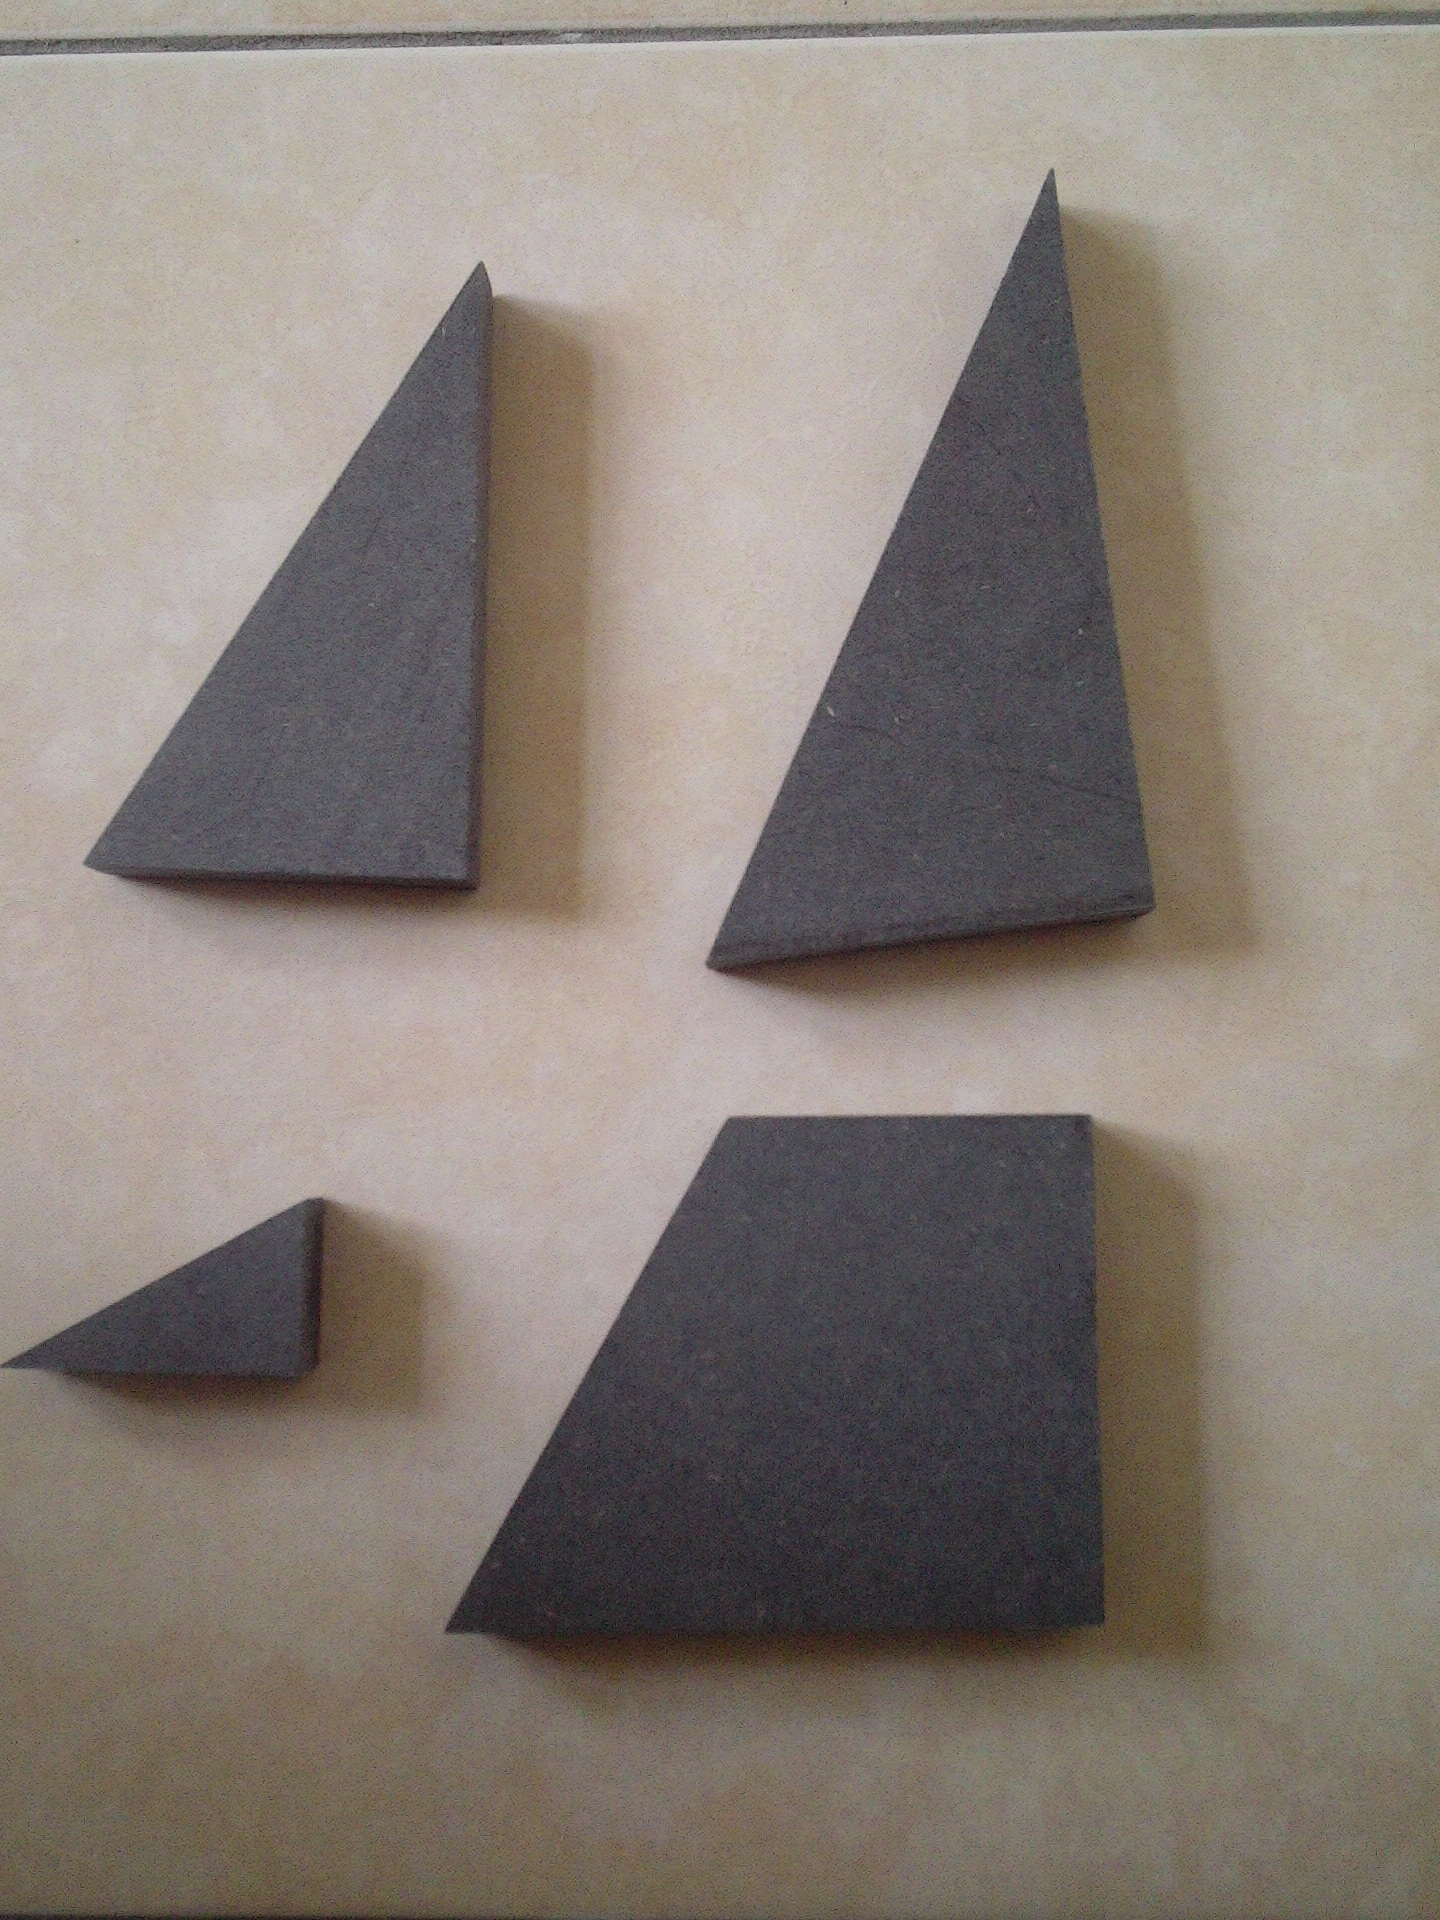
\includegraphics[height=7cm]{PIC0135}}
  \subfloat[]{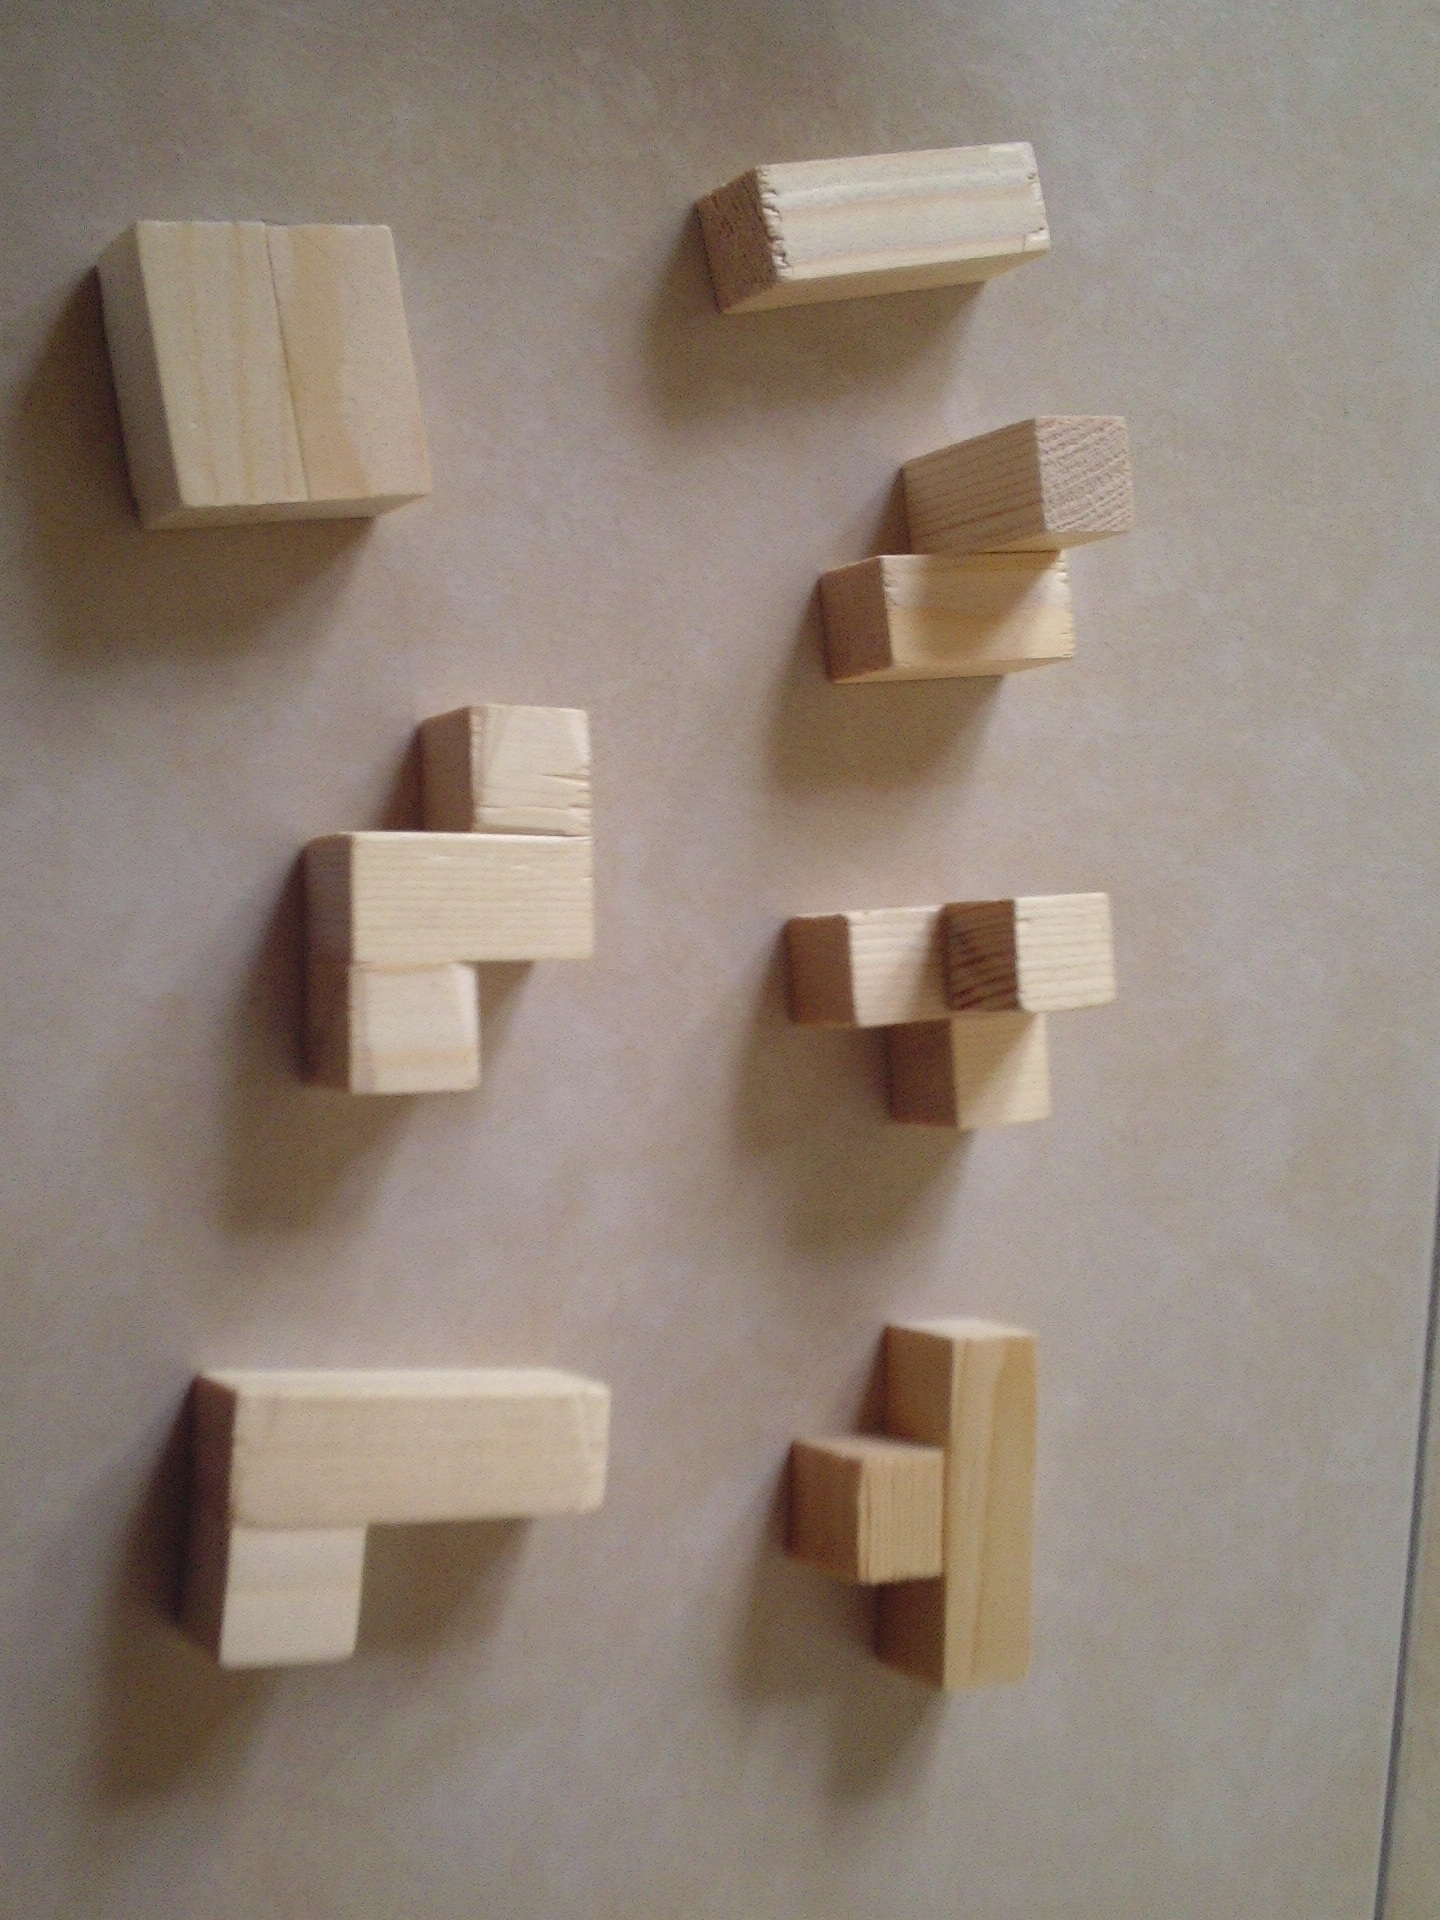
\includegraphics[height=7cm]{PIC0137}}\\
\end{figure}\\
\task{Leg deze blokken zo zodat je een vierkant krijgt.}\\
\task{Leg deze blokken zo zodat je een kubus krijgt.}
\subsection{Wordt vervolgd}
In de volgende les zullen we ons bezighouden met het vullen van vierkanten met vierkanten. Vervolgens zal het betegelen van een vlak met zeshoeken de leidraad zijn bij het vullen van een gegeven vlak.\\
\teacher{In de eerstkomende lessen zullen we het hebben over complete vlakvullingen (les over vierkanten vullen met vierkanten en perfecte vierkanten en de les over de meetkundige interpretaties van kwadratische vergelijkingen en kubische vergelijkingen).}
\newpage

\section{Perfecte Vierkanten}

\subsection{Vierkant vullen met vierkanten}

Nemen we een vierkant met zijde $10$, dan kan dit vierkant gevuld worden met $100$ kleinere vierkantjes van grootte $1$. Dit is duidelijk in Figuur \ref{fig:vierkant10_1x1}. Hetzelfde vierkant kunnen we ook vullen met vierkantjes van grootte $2$, waarbij we nu $25$ kleinere vierkantjes hebben in het grote vierkant. Als we nu echter dit vierkant compleet wensen te vullen met vierkantjes van grootte $3$, dan zien we dat dit niet lukt, zie Figuur \ref{fig:vierkant10_3x3}.

\begin{figure}[ht]
  \centering
  \subfloat[in vierkantjes met zijde $1$]{\label{fig:vierkant10_1x1}\definecolor{cqcqcq}{rgb}{0.75,0.75,0.75}
\begin{tikzpicture}[scale=0.45,line cap=round,line join=round,>=triangle 45,x=1.0cm,y=1.0cm]
\draw [color=cqcqcq,dash pattern=on 2pt off 2pt, xstep=1.0cm,ystep=1.0cm] (-0.5,-0.5) grid (10.5,10.5);
\clip(-0.5,-0.5) rectangle (10.5,10.5);
\filldraw[line width=1.6pt,fill=black,fill opacity=0.1] (0,0) -- (10,0) -- (10,10) -- (0,10) -- cycle;
\filldraw[fill=black,fill opacity=0.1] (0,0) -- (1,0) -- (1,1) -- (0,1) -- cycle;
\filldraw[fill=black,fill opacity=0.1] (1,0) -- (2,0) -- (2,1) -- (1,1) -- cycle;
\filldraw[fill=black,fill opacity=0.1] (2,0) -- (3,0) -- (3,1) -- (2,1) -- cycle;
\filldraw[fill=black,fill opacity=0.1] (3,0) -- (4,0) -- (4,1) -- (3,1) -- cycle;
\filldraw[fill=black,fill opacity=0.1] (4,0) -- (5,0) -- (5,1) -- (4,1) -- cycle;
\filldraw[fill=black,fill opacity=0.1] (5,0) -- (6,0) -- (6,1) -- (5,1) -- cycle;
\filldraw[fill=black,fill opacity=0.1] (6,0) -- (7,0) -- (7,1) -- (6,1) -- cycle;
\filldraw[fill=black,fill opacity=0.1] (7,0) -- (8,0) -- (8,1) -- (7,1) -- cycle;
\filldraw[fill=black,fill opacity=0.1] (8,0) -- (9,0) -- (9,1) -- (8,1) -- cycle;
\filldraw[fill=black,fill opacity=0.1] (9,0) -- (10,0) -- (10,1) -- (9,1) -- cycle;
\filldraw[fill=black,fill opacity=0.1] (0,1) -- (1,1) -- (1,2) -- (0,2) -- cycle;
\filldraw[fill=black,fill opacity=0.1] (1,1) -- (2,1) -- (2,2) -- (1,2) -- cycle;
\filldraw[fill=black,fill opacity=0.1] (2,1) -- (3,1) -- (3,2) -- (2,2) -- cycle;
\filldraw[fill=black,fill opacity=0.1] (3,1) -- (4,1) -- (4,2) -- (3,2) -- cycle;
\filldraw[fill=black,fill opacity=0.1] (4,1) -- (5,1) -- (5,2) -- (4,2) -- cycle;
\filldraw[fill=black,fill opacity=0.1] (5,1) -- (6,1) -- (6,2) -- (5,2) -- cycle;
\filldraw[fill=black,fill opacity=0.1] (6,1) -- (7,1) -- (7,2) -- (6,2) -- cycle;
\filldraw[fill=black,fill opacity=0.1] (7,1) -- (8,1) -- (8,2) -- (7,2) -- cycle;
\filldraw[fill=black,fill opacity=0.1] (8,1) -- (9,1) -- (9,2) -- (8,2) -- cycle;
\filldraw[fill=black,fill opacity=0.1] (9,1) -- (10,1) -- (10,2) -- (9,2) -- cycle;
\filldraw[fill=black,fill opacity=0.1] (0,2) -- (1,2) -- (1,3) -- (0,3) -- cycle;
\filldraw[fill=black,fill opacity=0.1] (1,2) -- (2,2) -- (2,3) -- (1,3) -- cycle;
\filldraw[fill=black,fill opacity=0.1] (2,2) -- (3,2) -- (3,3) -- (2,3) -- cycle;
\filldraw[fill=black,fill opacity=0.1] (3,2) -- (4,2) -- (4,3) -- (3,3) -- cycle;
\filldraw[fill=black,fill opacity=0.1] (4,2) -- (5,2) -- (5,3) -- (4,3) -- cycle;
\filldraw[fill=black,fill opacity=0.1] (5,2) -- (6,2) -- (6,3) -- (5,3) -- cycle;
\filldraw[fill=black,fill opacity=0.1] (6,2) -- (7,2) -- (7,3) -- (6,3) -- cycle;
\filldraw[fill=black,fill opacity=0.1] (7,2) -- (8,2) -- (8,3) -- (7,3) -- cycle;
\filldraw[fill=black,fill opacity=0.1] (8,2) -- (9,2) -- (9,3) -- (8,3) -- cycle;
\filldraw[fill=black,fill opacity=0.1] (9,2) -- (10,2) -- (10,3) -- (9,3) -- cycle;
\filldraw[fill=black,fill opacity=0.1] (0,3) -- (1,3) -- (1,4) -- (0,4) -- cycle;
\filldraw[fill=black,fill opacity=0.1] (1,3) -- (2,3) -- (2,4) -- (1,4) -- cycle;
\filldraw[fill=black,fill opacity=0.1] (2,3) -- (3,3) -- (3,4) -- (2,4) -- cycle;
\filldraw[fill=black,fill opacity=0.1] (3,3) -- (4,3) -- (4,4) -- (3,4) -- cycle;
\filldraw[fill=black,fill opacity=0.1] (4,3) -- (5,3) -- (5,4) -- (4,4) -- cycle;
\filldraw[fill=black,fill opacity=0.1] (5,3) -- (6,3) -- (6,4) -- (5,4) -- cycle;
\filldraw[fill=black,fill opacity=0.1] (6,3) -- (7,3) -- (7,4) -- (6,4) -- cycle;
\filldraw[fill=black,fill opacity=0.1] (7,3) -- (8,3) -- (8,4) -- (7,4) -- cycle;
\filldraw[fill=black,fill opacity=0.1] (8,3) -- (9,3) -- (9,4) -- (8,4) -- cycle;
\filldraw[fill=black,fill opacity=0.1] (9,3) -- (10,3) -- (10,4) -- (9,4) -- cycle;
\filldraw[fill=black,fill opacity=0.1] (0,4) -- (1,4) -- (1,5) -- (0,5) -- cycle;
\filldraw[fill=black,fill opacity=0.1] (1,4) -- (2,4) -- (2,5) -- (1,5) -- cycle;
\filldraw[fill=black,fill opacity=0.1] (2,4) -- (3,4) -- (3,5) -- (2,5) -- cycle;
\filldraw[fill=black,fill opacity=0.1] (3,4) -- (4,4) -- (4,5) -- (3,5) -- cycle;
\filldraw[fill=black,fill opacity=0.1] (4,4) -- (5,4) -- (5,5) -- (4,5) -- cycle;
\filldraw[fill=black,fill opacity=0.1] (5,4) -- (6,4) -- (6,5) -- (5,5) -- cycle;
\filldraw[fill=black,fill opacity=0.1] (6,4) -- (7,4) -- (7,5) -- (6,5) -- cycle;
\filldraw[fill=black,fill opacity=0.1] (7,4) -- (8,4) -- (8,5) -- (7,5) -- cycle;
\filldraw[fill=black,fill opacity=0.1] (8,4) -- (9,4) -- (9,5) -- (8,5) -- cycle;
\filldraw[fill=black,fill opacity=0.1] (9,4) -- (10,4) -- (10,5) -- (9,5) -- cycle;
\filldraw[fill=black,fill opacity=0.1] (0,5) -- (1,5) -- (1,6) -- (0,6) -- cycle;
\filldraw[fill=black,fill opacity=0.1] (1,5) -- (2,5) -- (2,6) -- (1,6) -- cycle;
\filldraw[fill=black,fill opacity=0.1] (2,5) -- (3,5) -- (3,6) -- (2,6) -- cycle;
\filldraw[fill=black,fill opacity=0.1] (3,5) -- (4,5) -- (4,6) -- (3,6) -- cycle;
\filldraw[fill=black,fill opacity=0.1] (4,5) -- (5,5) -- (5,6) -- (4,6) -- cycle;
\filldraw[fill=black,fill opacity=0.1] (5,5) -- (6,5) -- (6,6) -- (5,6) -- cycle;
\filldraw[fill=black,fill opacity=0.1] (6,5) -- (7,5) -- (7,6) -- (6,6) -- cycle;
\filldraw[fill=black,fill opacity=0.1] (7,5) -- (8,5) -- (8,6) -- (7,6) -- cycle;
\filldraw[fill=black,fill opacity=0.1] (8,5) -- (9,5) -- (9,6) -- (8,6) -- cycle;
\filldraw[fill=black,fill opacity=0.1] (9,5) -- (10,5) -- (10,6) -- (9,6) -- cycle;
\filldraw[fill=black,fill opacity=0.1] (0,6) -- (1,6) -- (1,7) -- (0,7) -- cycle;
\filldraw[fill=black,fill opacity=0.1] (1,6) -- (2,6) -- (2,7) -- (1,7) -- cycle;
\filldraw[fill=black,fill opacity=0.1] (2,6) -- (3,6) -- (3,7) -- (2,7) -- cycle;
\filldraw[fill=black,fill opacity=0.1] (3,6) -- (4,6) -- (4,7) -- (3,7) -- cycle;
\filldraw[fill=black,fill opacity=0.1] (4,6) -- (5,6) -- (5,7) -- (4,7) -- cycle;
\filldraw[fill=black,fill opacity=0.1] (5,6) -- (6,6) -- (6,7) -- (5,7) -- cycle;
\filldraw[fill=black,fill opacity=0.1] (6,6) -- (7,6) -- (7,7) -- (6,7) -- cycle;
\filldraw[fill=black,fill opacity=0.1] (7,6) -- (8,6) -- (8,7) -- (7,7) -- cycle;
\filldraw[fill=black,fill opacity=0.1] (8,6) -- (9,6) -- (9,7) -- (8,7) -- cycle;
\filldraw[fill=black,fill opacity=0.1] (9,6) -- (10,6) -- (10,7) -- (9,7) -- cycle;
\filldraw[fill=black,fill opacity=0.1] (0,7) -- (1,7) -- (1,8) -- (0,8) -- cycle;
\filldraw[fill=black,fill opacity=0.1] (1,7) -- (2,7) -- (2,8) -- (1,8) -- cycle;
\filldraw[fill=black,fill opacity=0.1] (2,7) -- (3,7) -- (3,8) -- (2,8) -- cycle;
\filldraw[fill=black,fill opacity=0.1] (3,7) -- (4,7) -- (4,8) -- (3,8) -- cycle;
\filldraw[fill=black,fill opacity=0.1] (4,7) -- (5,7) -- (5,8) -- (4,8) -- cycle;
\filldraw[fill=black,fill opacity=0.1] (5,7) -- (6,7) -- (6,8) -- (5,8) -- cycle;
\filldraw[fill=black,fill opacity=0.1] (6,7) -- (7,7) -- (7,8) -- (6,8) -- cycle;
\filldraw[fill=black,fill opacity=0.1] (7,7) -- (8,7) -- (8,8) -- (7,8) -- cycle;
\filldraw[fill=black,fill opacity=0.1] (8,7) -- (9,7) -- (9,8) -- (8,8) -- cycle;
\filldraw[fill=black,fill opacity=0.1] (9,7) -- (10,7) -- (10,8) -- (9,8) -- cycle;
\filldraw[fill=black,fill opacity=0.1] (0,8) -- (1,8) -- (1,9) -- (0,9) -- cycle;
\filldraw[fill=black,fill opacity=0.1] (1,8) -- (2,8) -- (2,9) -- (1,9) -- cycle;
\filldraw[fill=black,fill opacity=0.1] (2,8) -- (3,8) -- (3,9) -- (2,9) -- cycle;
\filldraw[fill=black,fill opacity=0.1] (3,8) -- (4,8) -- (4,9) -- (3,9) -- cycle;
\filldraw[fill=black,fill opacity=0.1] (4,8) -- (5,8) -- (5,9) -- (4,9) -- cycle;
\filldraw[fill=black,fill opacity=0.1] (5,8) -- (6,8) -- (6,9) -- (5,9) -- cycle;
\filldraw[fill=black,fill opacity=0.1] (6,8) -- (7,8) -- (7,9) -- (6,9) -- cycle;
\filldraw[fill=black,fill opacity=0.1] (7,8) -- (8,8) -- (8,9) -- (7,9) -- cycle;
\filldraw[fill=black,fill opacity=0.1] (8,8) -- (9,8) -- (9,9) -- (8,9) -- cycle;
\filldraw[fill=black,fill opacity=0.1] (9,8) -- (10,8) -- (10,9) -- (9,9) -- cycle;
\filldraw[fill=black,fill opacity=0.1] (0,9) -- (1,9) -- (1,10) -- (0,10) -- cycle;
\filldraw[fill=black,fill opacity=0.1] (1,9) -- (2,9) -- (2,10) -- (1,10) -- cycle;
\filldraw[fill=black,fill opacity=0.1] (2,9) -- (3,9) -- (3,10) -- (2,10) -- cycle;
\filldraw[fill=black,fill opacity=0.1] (3,9) -- (4,9) -- (4,10) -- (3,10) -- cycle;
\filldraw[fill=black,fill opacity=0.1] (4,9) -- (5,9) -- (5,10) -- (4,10) -- cycle;
\filldraw[fill=black,fill opacity=0.1] (5,9) -- (6,9) -- (6,10) -- (5,10) -- cycle;
\filldraw[fill=black,fill opacity=0.1] (6,9) -- (7,9) -- (7,10) -- (6,10) -- cycle;
\filldraw[fill=black,fill opacity=0.1] (7,9) -- (8,9) -- (8,10) -- (7,10) -- cycle;
\filldraw[fill=black,fill opacity=0.1] (8,9) -- (9,9) -- (9,10) -- (8,10) -- cycle;
\filldraw[fill=black,fill opacity=0.1] (9,9) -- (10,9) -- (10,10) -- (9,10) -- cycle;
\end{tikzpicture}
}
  \subfloat[in vierkantjes met zijde $2$]{\label{fig:vierkant10_2x2}\definecolor{cqcqcq}{rgb}{0.75,0.75,0.75}
\begin{tikzpicture}[scale=0.45,line cap=round,line join=round,>=triangle 45,x=1.0cm,y=1.0cm]
\draw [color=cqcqcq,dash pattern=on 2pt off 2pt, xstep=1.0cm,ystep=1.0cm] (-0.5,-0.5) grid (10.5,10.5);
\clip(-0.5,-0.5) rectangle (10.5,10.5);
\filldraw[line width=1.6pt,fill=black,fill opacity=0.1] (0,0) -- (10,0) -- (10,10) -- (0,10) -- cycle;
\filldraw[fill=black,fill opacity=0.1] (0,0) -- (2,0) -- (2,2) -- (0,2) -- cycle;
\filldraw[fill=black,fill opacity=0.1] (2,0) -- (4,0) -- (4,2) -- (2,2) -- cycle;
\filldraw[fill=black,fill opacity=0.1] (4,0) -- (6,0) -- (6,2) -- (4,2) -- cycle;
\filldraw[fill=black,fill opacity=0.1] (6,0) -- (8,0) -- (8,2) -- (6,2) -- cycle;
\filldraw[fill=black,fill opacity=0.1] (8,0) -- (10,0) -- (10,2) -- (8,2) -- cycle;
\filldraw[fill=black,fill opacity=0.1] (0,2) -- (2,2) -- (2,4) -- (0,4) -- cycle;
\filldraw[fill=black,fill opacity=0.1] (2,2) -- (4,2) -- (4,4) -- (2,4) -- cycle;
\filldraw[fill=black,fill opacity=0.1] (4,2) -- (6,2) -- (6,4) -- (4,4) -- cycle;
\filldraw[fill=black,fill opacity=0.1] (6,2) -- (8,2) -- (8,4) -- (6,4) -- cycle;
\filldraw[fill=black,fill opacity=0.1] (8,2) -- (10,2) -- (10,4) -- (8,4) -- cycle;
\filldraw[fill=black,fill opacity=0.1] (0,4) -- (2,4) -- (2,6) -- (0,6) -- cycle;
\filldraw[fill=black,fill opacity=0.1] (2,4) -- (4,4) -- (4,6) -- (2,6) -- cycle;
\filldraw[fill=black,fill opacity=0.1] (4,4) -- (6,4) -- (6,6) -- (4,6) -- cycle;
\filldraw[fill=black,fill opacity=0.1] (6,4) -- (8,4) -- (8,6) -- (6,6) -- cycle;
\filldraw[fill=black,fill opacity=0.1] (8,4) -- (10,4) -- (10,6) -- (8,6) -- cycle;
\filldraw[fill=black,fill opacity=0.1] (0,6) -- (2,6) -- (2,8) -- (0,8) -- cycle;
\filldraw[fill=black,fill opacity=0.1] (2,6) -- (4,6) -- (4,8) -- (2,8) -- cycle;
\filldraw[fill=black,fill opacity=0.1] (4,6) -- (6,6) -- (6,8) -- (4,8) -- cycle;
\filldraw[fill=black,fill opacity=0.1] (6,6) -- (8,6) -- (8,8) -- (6,8) -- cycle;
\filldraw[fill=black,fill opacity=0.1] (8,6) -- (10,6) -- (10,8) -- (8,8) -- cycle;
\filldraw[fill=black,fill opacity=0.1] (0,8) -- (2,8) -- (2,10) -- (0,10) -- cycle;
\filldraw[fill=black,fill opacity=0.1] (2,8) -- (4,8) -- (4,10) -- (2,10) -- cycle;
\filldraw[fill=black,fill opacity=0.1] (4,8) -- (6,8) -- (6,10) -- (4,10) -- cycle;
\filldraw[fill=black,fill opacity=0.1] (6,8) -- (8,8) -- (8,10) -- (6,10) -- cycle;
\filldraw[fill=black,fill opacity=0.1] (8,8) -- (10,8) -- (10,10) -- (8,10) -- cycle;
\end{tikzpicture}
}
  \subfloat[in vierkantjes met zijde $3$]{\label{fig:vierkant10_3x3}\definecolor{cqcqcq}{rgb}{0.75,0.75,0.75}
\begin{tikzpicture}[scale=0.4,line cap=round,line join=round,>=triangle 45,x=1.0cm,y=1.0cm]
\draw [color=cqcqcq,dash pattern=on 2pt off 2pt, xstep=1.0cm,ystep=1.0cm] (-0.5,-0.5) grid (10.5,10.5);
\clip(-0.5,-0.5) rectangle (10.5,10.5);
\filldraw[line width=1.6pt,fill=black,fill opacity=0.1] (0,0) -- (10,0) -- (10,10) -- (0,10) -- cycle;
\filldraw[fill=black,fill opacity=0.1] (0,0) -- (3,0) -- (3,3) -- (0,3) -- cycle;
\filldraw[fill=black,fill opacity=0.1] (3,0) -- (6,0) -- (6,3) -- (3,3) -- cycle;
\filldraw[fill=black,fill opacity=0.1] (6,0) -- (9,0) -- (9,3) -- (6,3) -- cycle;
\filldraw[fill=black,fill opacity=0.1] (0,3) -- (3,3) -- (3,6) -- (0,6) -- cycle;
\filldraw[fill=black,fill opacity=0.1] (3,3) -- (6,3) -- (6,6) -- (3,6) -- cycle;
\filldraw[fill=black,fill opacity=0.1] (6,3) -- (9,3) -- (9,6) -- (6,6) -- cycle;
\filldraw[fill=black,fill opacity=0.1] (0,6) -- (3,6) -- (3,9) -- (0,9) -- cycle;
\filldraw[fill=black,fill opacity=0.1] (3,6) -- (6,6) -- (6,9) -- (3,9) -- cycle;
\filldraw[fill=black,fill opacity=0.1] (6,6) -- (9,6) -- (9,9) -- (6,9) -- cycle;
\end{tikzpicture}
}
  \caption{Verdelen van een vierkant met zijde $10$.}
  \label{fig:vierkant10}
\end{figure}

We kunnen het vierkant met zijde $10$ vullen met $9$ vierkanten van zijde $3$. Er blijven $19$ kleinere vierkantjes van zijde $1$ over. We kunnen dit ook als volgt zien: als we de zijde van grootte $10$ delen door de grootte van de kleinere zijde $3$, dan is de rest $1$ en het quotiënt $3$. We hebben dus
$$
10 = 3\cdot 3 + 1.
$$
Het gaat uiteraard over vierkanten. Dus om met de oppervlakten te werken moeten we links en rechts kwadrateren, we krijgen dus
\begin{align*}
  10^2  &= (3\cdot 3 + 1)^2\\
  \Leftrightarrow 100   &= (3\cdot 3)^2 + 2\cdot 3\cdot 3\cdot 1 + 1^2\\
  \Leftrightarrow 100   &= 81 + 19
\end{align*}

In het linkerlid staat dus de oppervlakte van het groter vierkant. Het rechter lid is opgesplitst in het totale oppervlakte van de kleinere vierkanten plus wat er nog overblijft als rest.

Vul nu zelf de vierkanten met zijde $9$ uit Figuur \ref{fig:vierkant9}. Eerst met kleinere vierkantjes van grootte $1$, dan met kleinere vierkantjes van grootte $2$ en uiteindelijk met kleinere vierkantjes van grootte $3$. Gebruik wat je kent over delen van getallen en rest bij deling om het resultaat te verklaren.

\begin{figure}[ht]
  \centering
  \subfloat[in vierkantjes met zijde $1$]{\definecolor{cqcqcq}{rgb}{0.75,0.75,0.75}
\begin{tikzpicture}[scale=0.45,line cap=round,line join=round,>=triangle 45,x=1.0cm,y=1.0cm]
\draw [color=cqcqcq,dash pattern=on 2pt off 2pt, xstep=1.0cm,ystep=1.0cm] (-0.5,-0.5) grid (9.5,9.5);
\clip(-0.5,-0.5) rectangle (9.5,9.5);
\filldraw[line width=1.6pt,fill=black,fill opacity=0.1] (0,0) -- (9,0) -- (9,9) -- (0,9) -- cycle;
\end{tikzpicture}
}
  \subfloat[in vierkantjes met zijde $2$]{\definecolor{cqcqcq}{rgb}{0.75,0.75,0.75}
\begin{tikzpicture}[scale=0.45,line cap=round,line join=round,>=triangle 45,x=1.0cm,y=1.0cm]
\draw [color=cqcqcq,dash pattern=on 2pt off 2pt, xstep=1.0cm,ystep=1.0cm] (-0.5,-0.5) grid (9.5,9.5);
\clip(-0.5,-0.5) rectangle (9.5,9.5);
\filldraw[line width=1.6pt,fill=black,fill opacity=0.1] (0,0) -- (9,0) -- (9,9) -- (0,9) -- cycle;
\end{tikzpicture}
}
  \subfloat[in vierkantjes met zijde $3$]{\definecolor{cqcqcq}{rgb}{0.75,0.75,0.75}
\begin{tikzpicture}[scale=0.45,line cap=round,line join=round,>=triangle 45,x=1.0cm,y=1.0cm]
\draw [color=cqcqcq,dash pattern=on 2pt off 2pt, xstep=1.0cm,ystep=1.0cm] (-0.5,-0.5) grid (9.5,9.5);
\clip(-0.5,-0.5) rectangle (9.5,9.5);
\filldraw[line width=1.6pt,fill=black,fill opacity=0.1] (0,0) -- (9,0) -- (9,9) -- (0,9) -- cycle;
\end{tikzpicture}
}
  \caption{Verdelen van een vierkant met zijde $9$.}
  \label{fig:vierkant9}
\end{figure}

Verklaring:
\answer[4cm]{Elk vierkant waarvan de zijden een natuurlijke (dus geen komma getallen) grootte hebben volledig opgevuld worden met kleinere vierkantjes van grootte $1$. Omdat $9$ niet deelbaar is door $2$ blijven we met een rest zitten. We kunnen deze rest als volgt berekenen: de rest bij deling van $9$ door $2$ is $1$ en het quotiënt is $4$,  we hebben dus $9=4\cdot 2 + 1$, dit links en rechts kwadrateren geeft $9^2=(4\cdot 2 + 1)^2\Leftrightarrow 9^2=(4\cdot 2)^2 + 2\cdot 4\cdot 2 + 1^2 \Leftrightarrow 81 = 64 + 16 + 1 \Leftrightarrow 81 = 64 + 17$. Het vierkant van zijde $9$ vullen met vierkanten van zijde $3$ lukt volledig omdat $3$ een deler is van $9$.}

We kunnen dit gaan veralgemenen voor een groot vierkant met zijde $a$ en kleinere vierkanten met zijde $d$. Er zal dus steeds gelden
$$
a = q\cdot d + r
$$
waarbij $q$ het aantal keer is dat we $d$ in $a$ krijgen en $r$ de rest is die dan nog overblijft. Als we dit dan links en rechts kwadrateren, dan krijgen we
\begin{align*}
  a^2  &= (q\cdot d + r)^2\\
  \Leftrightarrow a^2   &= (q\cdot d)^2 + 2\cdot q\cdot d\cdot r + r^2\;.\\
\end{align*}
In een groot vierkant zal de oppervlakte dus $a^2$ zijn en het wordt gevuld met $q^2$ kleinere vierkanten van oppervlakte $d^2$. In het totaal blijft een oppervlakte van $2\cdot q\cdot r + r^2$ over. Laten we deze restoppervlakte nu de overschot noemen. Dit kunnen we ontleden in een stukje oppervlakte van $q\cdot r$ dat rechts overblijft, een stukje oppervlakte van $q\cdot r$ dat bovenaan overblijft en een stukje oppervlakte $r^2$ dat rechtsboven overblijft.

Duid deze nog aan op Figuur \ref{fig:vierkant10_4x4} waarbij een groot vierkant met zijde $10$ werd opgedeeld in vierkanten met zijde $4$.
\answer{Het blauwe en rode stukje hebben oppervlakte $q\cdot r$, het groene stukje heeft oppervlakte $r^2$.}

\begin{figure}[ht]
  \centering
  \definecolor{zzccqq}{rgb}{0.6,0.8,0}
\definecolor{wwwwff}{rgb}{0.4,0.4,1}
\definecolor{ffwwtt}{rgb}{1,0.4,0.2}
\definecolor{cqcqcq}{rgb}{0.75,0.75,0.75}
\begin{tikzpicture}[scale=0.6,line cap=round,line join=round,>=triangle 45,x=1.0cm,y=1.0cm]
\draw [color=cqcqcq,dash pattern=on 1pt off 1pt, xstep=1.0cm,ystep=1.0cm] (-0.5,-0.5) grid (10.5,10.5);
\clip(-0.5,-0.5) rectangle (10.5,10.5);
\filldraw[fill=black,fill opacity=0.1] (0,0) -- (10,0) -- (10,10) -- (0,10) -- cycle;
\filldraw[fill=black,fill opacity=0.1] (0,0) -- (4,0) -- (4,4) -- (0,4) -- cycle;
\filldraw[fill=black,fill opacity=0.1] (4,0) -- (8,0) -- (8,4) -- (4,4) -- cycle;
\filldraw[fill=black,fill opacity=0.1] (0,4) -- (4,4) -- (4,8) -- (0,8) -- cycle;
\filldraw[fill=black,fill opacity=0.1] (4,4) -- (8,4) -- (8,8) -- (4,8) -- cycle;
\filldraw[color=ffwwtt,fill=ffwwtt,fill opacity=0.1] (8,0) -- (10,0) -- (10,8) -- (8,8) -- cycle;
\filldraw[color=wwwwff,fill=wwwwff,fill opacity=0.1] (0,10) -- (0,8) -- (8,8) -- (8,10) -- cycle;
\filldraw[color=zzccqq,fill=zzccqq,fill opacity=0.1] (8,8) -- (10,8) -- (10,10) -- (8,10) -- cycle;
\filldraw [color=ffwwtt] (8,0)-- (10,0);
\draw [color=ffwwtt] (10,0)-- (10,8);
\draw [color=ffwwtt] (10,8)-- (8,8);
\draw [color=ffwwtt] (8,8)-- (8,0);
\draw [color=wwwwff] (0,10)-- (0,8);
\draw [color=wwwwff] (0,8)-- (8,8);
\draw [color=wwwwff] (8,8)-- (8,10);
\draw [color=wwwwff] (8,10)-- (0,10);
\draw [color=zzccqq] (8,8)-- (10,8);
\draw [color=zzccqq] (10,8)-- (10,10);
\draw [color=zzccqq] (10,10)-- (8,10);
\draw [color=zzccqq] (8,10)-- (8,8);
\end{tikzpicture}

  \caption{Rest van een vierkant van grootte 10 verdeeld in vierkantjes van grootte 4.}
  \label{fig:vierkant10_4x4}
\end{figure}

\newpage
\subsection{Perfecte vierkanten}

Het probleem om een vierkant te vullen met kleinere vierkanten wordt heel wat uitdagender en een gans stuk moeilijker als we eisen dat alle vierkanten een andere grootte moeten hebben. Indien een vierkant volledig gevuld wordt met kleinere vierkanten die allemaal een andere grootte hebben, dan spreken we van een {\bf perfect vierkant}. Het aantal kleinere vierkanten dat het grootte vierkant bevat wordt de {\bf orde} van het perfecte vierkant genoemd. Het vierkant met de kleinste orde staat in Figuur \ref{fig:pv21}.

\begin{figure}[ht]
  \centering
  {\small
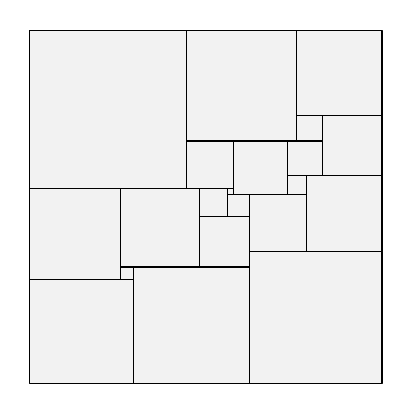
\begin{tikzpicture}[scale=0.04,line cap=round,line join=round,>=triangle 45,x=1.0cm,y=1.0cm]
\clip(-0.5,-0.5) rectangle (113,113);
\filldraw[fill=black,fill opacity=0.05] (0,0) -- (33,0) -- (33,33) -- (0,33) -- cycle;
\filldraw[fill=black,fill opacity=0.05] (33,0) -- (70,0) -- (70,37) -- (33,37) -- cycle;
\filldraw[fill=black,fill opacity=0.05] (70,0) -- (112,0) -- (112,42) -- (70,42) -- cycle;
\filldraw[fill=black,fill opacity=0.05] (0,33) -- (29,33) -- (29,62) -- (0,62) -- cycle;
\filldraw[fill=black,fill opacity=0.05] (29,33) -- (33,33) -- (33,37) -- (29,37) -- cycle;
\filldraw[fill=black,fill opacity=0.05] (0,62) -- (50,62) -- (50,112) -- (0,112) -- cycle;
\filldraw[fill=black,fill opacity=0.05] (29,62) -- (29,37) -- (54,37) -- (54,62) -- cycle;
\filldraw[fill=black,fill opacity=0.05] (54,37) -- (70,37) -- (70,53) -- (54,53) -- cycle;
\filldraw[fill=black,fill opacity=0.05] (70,42) -- (88,42) -- (88,60) -- (70,60) -- cycle;
\filldraw[fill=black,fill opacity=0.05] (88,42) -- (112,42) -- (112,66) -- (88,66) -- cycle;
\filldraw[fill=black,fill opacity=0.05] (54,53) -- (63,53) -- (63,62) -- (54,62) -- cycle;
\filldraw[fill=black,fill opacity=0.05] (63,53) -- (70,53) -- (70,60) -- (63,60) -- cycle;
\filldraw[fill=black,fill opacity=0.05] (63,60) -- (65,60) -- (65,62) -- (63,62) -- cycle;
\filldraw[fill=black,fill opacity=0.05] (82,60) -- (88,60) -- (88,66) -- (82,66) -- cycle;
\filldraw[fill=black,fill opacity=0.05] (65,60) -- (82,60) -- (82,77) -- (65,77) -- cycle;
\filldraw[fill=black,fill opacity=0.05] (50,62) -- (65,62) -- (65,77) -- (50,77) -- cycle;
\filldraw[fill=black,fill opacity=0.05] (50,112) -- (50,77) -- (85,77) -- (85,112) -- cycle;
\filldraw[fill=black,fill opacity=0.05] (82,77) -- (82,66) -- (93,66) -- (93,77) -- cycle;
\filldraw[fill=black,fill opacity=0.05] (93,66) -- (112,66) -- (112,85) -- (93,85) -- cycle;
\filldraw[fill=black,fill opacity=0.05] (85,77) -- (93,77) -- (93,85) -- (85,85) -- cycle;
\filldraw[fill=black,fill opacity=0.05] (85,85) -- (112,85) -- (112,112) -- (85,112) -- cycle;
\end{tikzpicture}
}

  \caption{Perfect vierkant van orde $21$.}
  \label{fig:pv21}
\end{figure}

Het vierkant van de kleinste orde vinden bleek een uitdagend probleem waarop wiskundigen ongeveer 60 jaar gezocht hebben! Alles begon in 1902, toen een zekere {\it Dudeney} een raadseltje publiceerde waarbij gevraagd werd om een vierkant te verdelen in allemaal verschillende vierkanten en één rechthoek. Zijn raadseltje noemde hij {\it De juwelenbox van Mejuffrouw Isabel}.














\newpage
\section{Tweedimensionale stapelproblemen}

\subsection{Algemeen}
In de voorbije lessen hebben we het vooral gehad over complete vlakvullingen, i.h.b. het vullen van vlakken met vierkanten. 
In dit onderdeel zullen we kijken naar het vullen van vlakken met figuren die het vlak nooit volledig zullen vullen. We noemen dit dan een tweedimensionale stapelprobleem. We zijn namelijk op weg om het bolstapelprobleem van Kepler te bekijken!

Bij het stapelen in twee dimensies hebben we minder mogelijkheden dan bij het stapelen in drie dimensies, maar we kunnen er toch heel veel over zeggen. Als we denken aan tweedimensionale stapelingen, dan denken we aan een vlak waarin we voorwerpen stapelen die twee dimensies hebben. Deze voorwerpen kunnen heel uiteenlopend zijn. Naar analogon met het bolstapelprobleem van Kepler waarbij we met bollen zullen werken bekijken we het geval van de cirkels. 


In de eerste les hebben we reeds gezien dat je een oneindig vlak volledig kan vullen met identieke gelijkzijdige driehoeken, vierkanten en zeshoeken. Dit noemen we 100\% effici�ntie. 

\ask{Hebben we ook 100\% effici�ntie als we een oneindig vlak zouden betegelen met cirkels?}

\answer[2cm]{Neen, want cirkels hebben geen rechte zijde om ze aan elkaar te plaatsen.}

Het antwoord is natuurlijk 'neen'. Maar wat is de effici�ntie dan wel? En in welke configuratie is deze het beste?

\task{Probeer cirkels (munten, flippo's, pokerjetons ...) eens zodanig op een tafel te leggen dat er zo weinig mogelijk ruimte tussen de cirkels overblijft.}

Het was reeds duidelijk je nooit elk plekje van de tafel kunt bedekken als de cirkels elkaar niet mogen overlappen.

We zijn in eerste instantie ge�nteresseerd in rangschikkingen van oneindig veel cirkels op een oneindige grote tafel. Je hoeft dan geen rekening te houden met wat er aan de randen gebeurt. De randen maken alles moeilijker (maar ook interessanter, iets waar we later nog op zullen terug komen). E�n voor de hand liggende mogelijkheid om de cirkels zo effici�nt mogelijk in het vlak te rangschikken is om ze netjes naast en boven elkaar te leggen, volgens een patroon van vierkantjes. Dat dit niet de best mogelijke oplossing is wordt al snel duidelijk door wat met de rijen te schuiven. Je kunt de rijen namelijk iets beter in elkaar laten passen. Iedere cirkel raakt dan aan zes andere cirkels \todo{Vermelden van kissingnumber?}, in plaats van aan vier, zoals in het vierkante geval. De cirkels komen nu in een regelmatig patroon te liggen op een zogenaamd hexagonaal rooster. Het lijkt onmogelijk om de cirkels nog dichter bij elkaar te krijgen. Dat dit inderdaad niet beter kan werd ongeveer honderd jaar geleden bewezen door de Deense getaltheoreticus Thue. Een schets van het bewijs zullen we zo meteen bekijken. Eerst gaan wij zelf op zoek naar wat nu juist de effici�ntie is en hoe je deze moet berekenen.

\subsection{Voronoicellen}

Om te berekenen hoe effici�nt een schikking met cirkels is, maken we gebruik van Voronoicellen. De {\bf Voronoicel} van een cirkel is de verzameling van alle punten die dichter bij het middelpunt van deze cirkel liggen dan bij het middelpunt van elke andere cirkel in de schikking.

\ask{Hoe ziet de Voronoicel eruit bij een vierkante rangschikking? Hoe ziet de Voronoicel eruit bij de hexagonale rangschikking?}

\answer[2cm]{Bij de vierkante rangschikking is zo'n Voronoicel een vierkant dat strak om de cirkel zit, en voor de hexagonale rangschikking is het een regelmatige zeshoek.}

\ask{Hoe kan je de effici�ntie berekenen aan de hand van zo'n Voronoicel?}

\answer[3cm]{Het percentage van het vlak dat wordt bedekt door de cirkels is gelijk aan het percentage van de Voronoicel dat door ��n cirkel wordt bedekt, want voor alle cirkels is de vorm van de Voronoicel hetzelfde en de Voronoicellen betegelen samen het hele vlak.}

\task{Bereken voor de vierkante en de hexagonale rangschikking de effici�ntie.}

\begin{enumerate}
	\item \textbf{Vierkante rangschikking}:\\
	\answer[2cm]{Als je cirkels neemt met straal gelijk aan 1, dan heeft het strakke 'omgeschreven' vierkant in de vierkante betegeling een zijde met lengte 2. De oppervlakte van de cirkel hier is $\pi$, de oppervlakte van het vierkant is 4. (Uiteraard konden we andere afmetingen genomen hebben, maar de verhoudingen blijven steeds hetzelfde.) Er is dus $\frac{\pi}{4}=0,78538...$, of ruim 78\% van het totale vlak bedekt door de cirkels.}
	\item \textbf{Hexagonale rangschikking}:\\
	\answer[2cm]{De zeshoek om een cirkel met straal 1 kan worden opgedeeld in twaalf halve gelijkzijdige driehoekjes met een basis met lengte 1 en een hoogte van $\frac{1}{\sqrt{3}}$. De oppervlakte van de zeshoek is dus $12.\frac{1}{2}.1.\frac{1}{\sqrt{3}}=2\sqrt{3}$. De effici�ntie of bedekkingsgraad is dus $\frac{\pi}{\sqrt{12}}=0.90689$.}
\end{enumerate}


\begin{figure}[h]
  \centering
  \subfloat[]{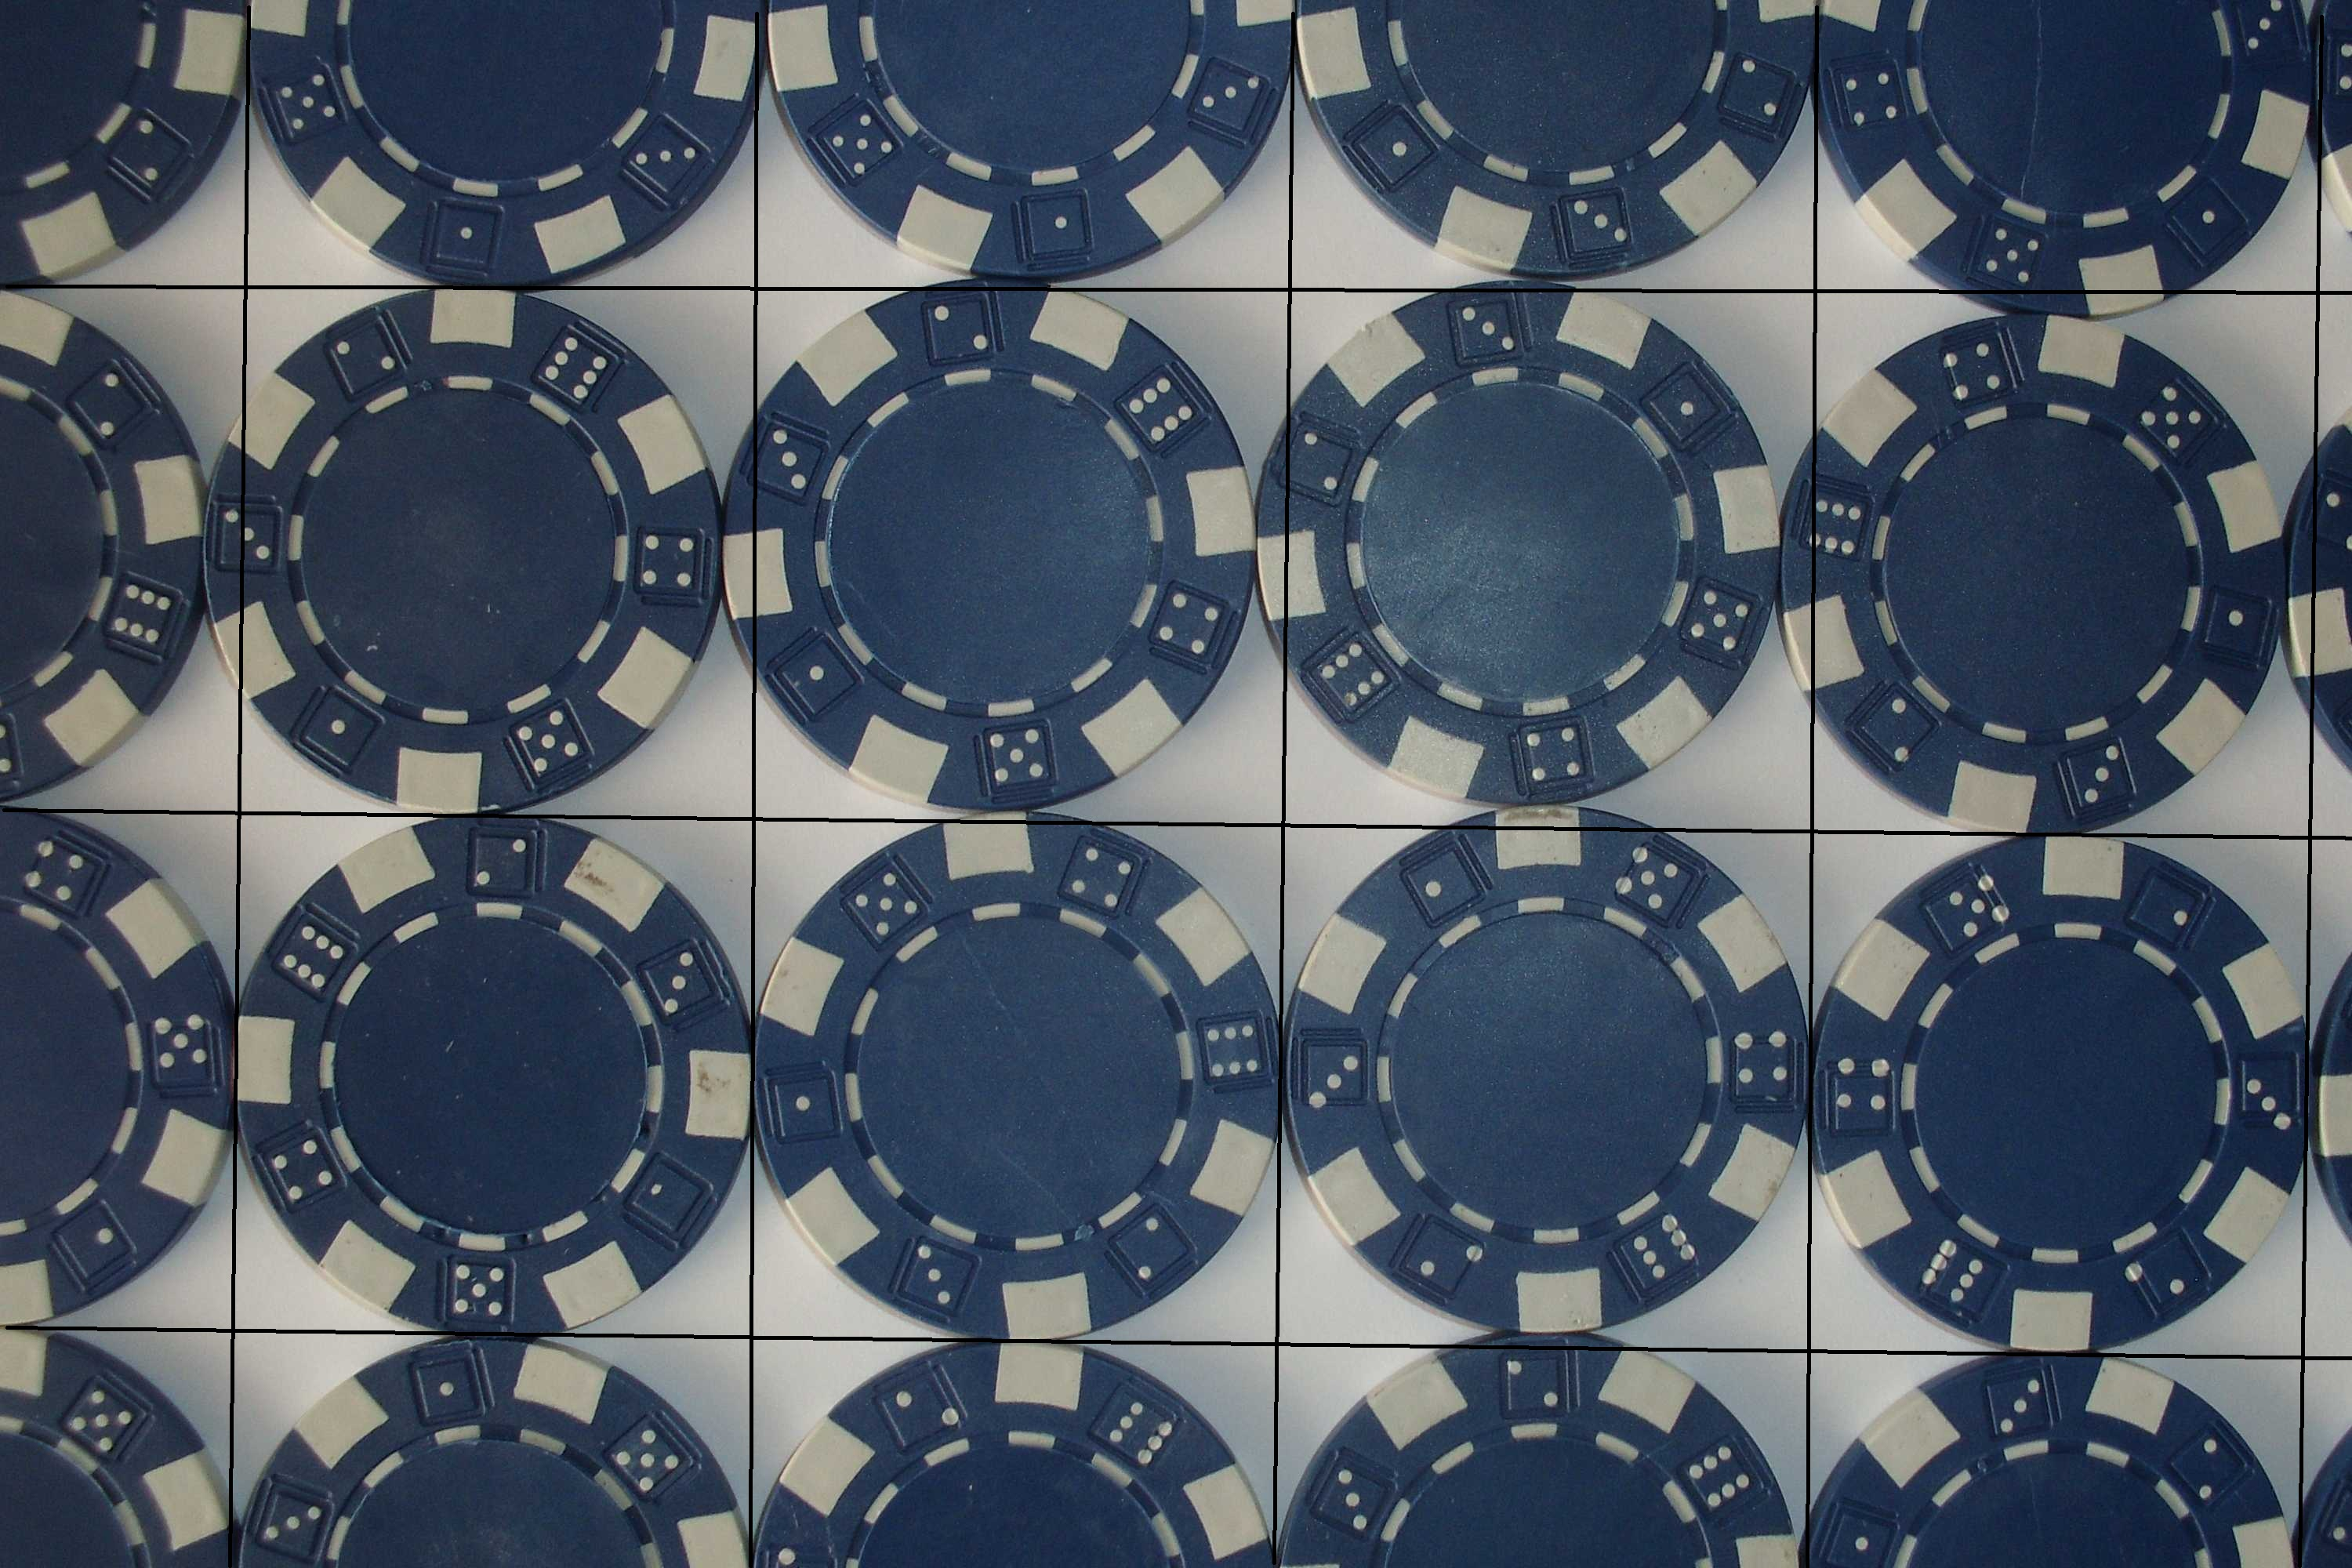
\includegraphics[width=0.45\textwidth]{voronoi_sqr}\label{vs}}\qquad
  \subfloat[]{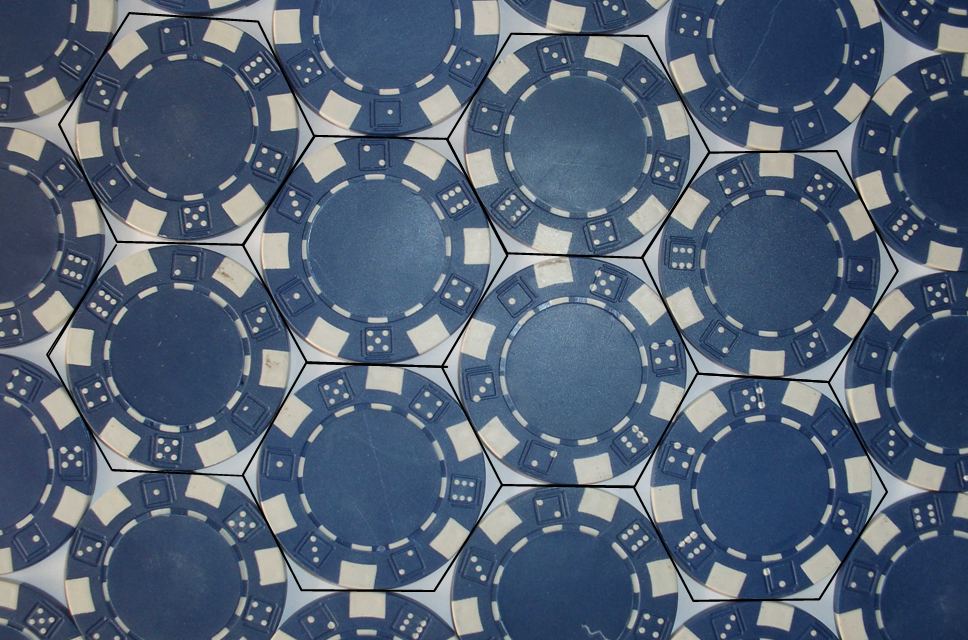
\includegraphics[width=0.45\textwidth]{voronoi_hex}\label{vh}}
  \caption{Vierkante en hexagonale rangschikking met pokerjetons en hun voronoicellen}  
\end{figure}


\subsection{Axel Thue}
De Scandinavische wiskundige Axel Thue (1863-1922) ontwikkelde in 1892 een theorie over het tweedimensionale equivalent voor 'het probleem van Kepler' waarin men zocht naar de dichtste pakkingsmethode voor cirkels in het vlak. Thue betegelde het vlak met identieke gelijkzijdige zeshoeken en tekende in elke zeshoek een cirkel op zo'n manier dat elke cirkel alle zijden van de zeshoek raakte. Hierdoor verkreeg hij een dichtheid van 90.69\%, waarvan hij beweerde dat dit de hoogst mogelijke dichtheid was bij het stapelen in 2 dimensies. 
Om dit te bewijzen tekende Thue een begrensd aantal cirkels met straal 1 die elkaar niet overlapten. Daarna verdeelde hij willekeurig het tweedimensionale vlak in bepaalde gebieden waarbij hij aantoonde dat de dichtheid in elk gebied maximum 90.69\% is. Hierdoor bestond er geen tweedimensionale pakking waarbij de dichtheid groter is dan 90.69\% en op die manier bewees Thue zijn vermoeden dat de hexagonale pakking de dichtste pakkingsmethode was in twee dimensies.
Het volledige bewijs zullen we hier niet meer bespreken, maar we zullen wel even kijken hoe Thue het vlak waarin de cirkels liggen heeft opgedeeld in verschillende gebieden. Hiervoor zullen we een korte vertaling geven van een deel van het oorspronkelijke Engelstalige bewijs dat geschreven is door Axel Thue.

\begin{quotation}
``Teken een grotere cirkel met straal $\frac{2}{\sqrt{3}}$ rond elke cirkel (zie figuur \ref{2D1}). Telkens als twee van deze grote cirkels elkaar snijden, teken je het lijnstuk tussen de twee snijpunten, waarna je twee congruente driehoeken construeert met het lijnstuk als basis en de tophoeken in het centrum van de cirkels (zie figuur \ref{2D2}). Er zal nooit een punt zijn dat tegelijk binnen alle drie de cirkels ligt. Zoals we merken in figuur \ref{2D3} zullen drie grote cirkels elkaar maximum in ��n punt snijden, het cirkelcentrum, als de centra van de drie grote cirkels de tophoeken zijn van een gelijkzijdige driehoek met zijde 2. \\
Dit geeft ons de verdeling van de ruimte: gebieden buiten de grote cirkels (wit), de gelijkbenige driehoeken (groenachtig blauw), en het gedeelte binnen de grote cirkels, maar buiten de driehoeken (lichtpaars) (zie figuur \ref{2D4}).''
\end{quotation}


\begin{figure}[h]
  \centering
  \subfloat[]{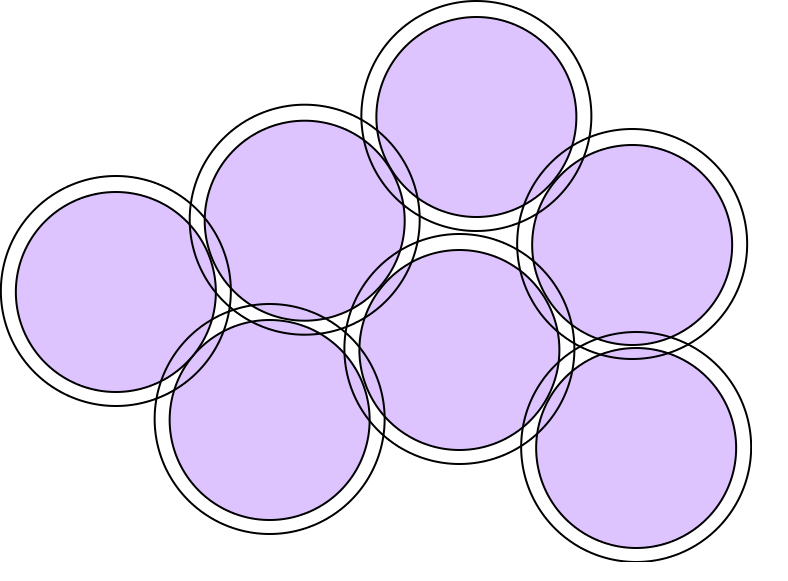
\includegraphics[height=3cm]{2D1}\label{2D1}}
  \subfloat[]{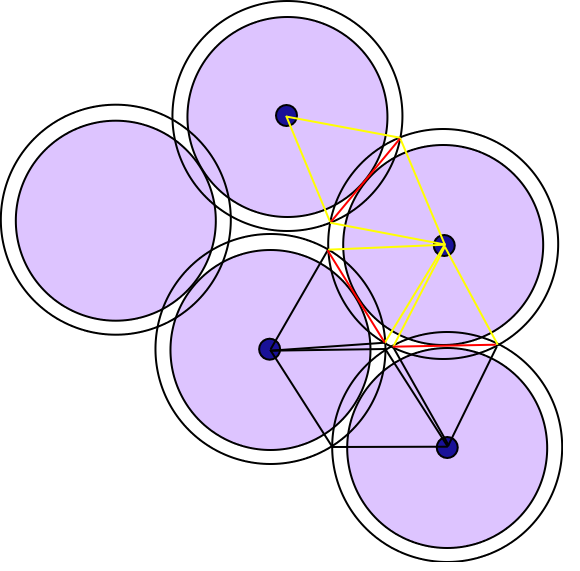
\includegraphics[height=3cm]{2D2}\label{2D2}}
  \subfloat[]{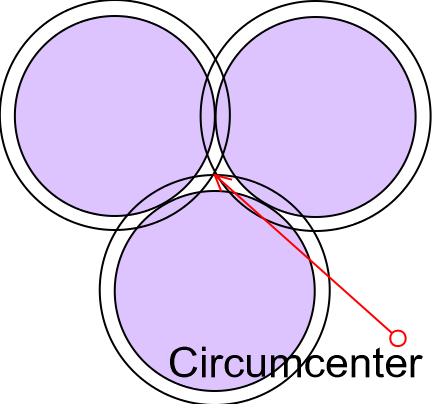
\includegraphics[height=3cm]{2D3}\label{2D3}}
  \subfloat[]{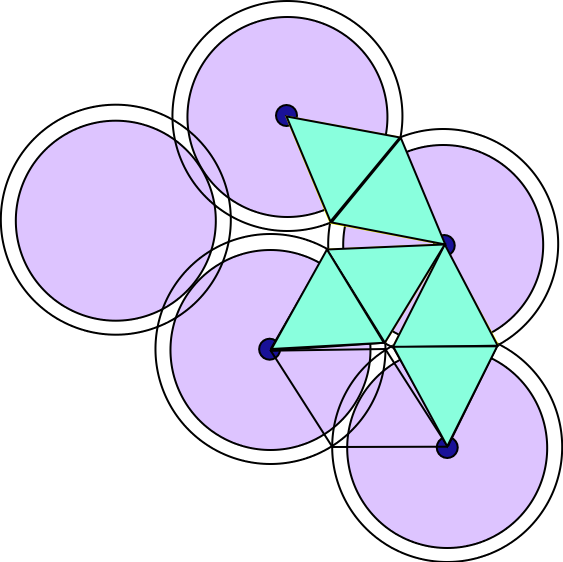
\includegraphics[height=3cm]{2D4}\label{2D4}}\\
  \caption{Figuren bij bewijs van Axel Thue}  
\end{figure}

Uit deze vertaling concluderen we dus dat Thue zijn vlak in 3 gebieden opgedeeld heeft. Hierna zal hij nog berekenen hoeveel oppervlakte er in de drie gebieden wordt ingenomen door de cirkels en uiteindelijk zal hij tot de conclusie komen dat geen enkel gebied een dichtheid heeft van meer dan 90.69\%, waardoor het bewijs voor het tweedimensionale equivalent van het bolstapelprobleem is afgerond.


\subsection{Dienbladenprobleem}
Bij de meeste stapelingen stelt men zich de vraag hoeveel identieke voorwerpen men in een ruimte met vastgelegde grenzen kan stoppen. Wij zullen de vraag omkeren. In ons praktische probleem vragen we ons af wat de meest compacte ruimte is voor een vastgelegd aantal identieke voorwerpen.
We kunnen dit probleem als volgt bekijken: een fabrikant wil dienbladen voor een bepaalde aantal glazen of blikjes. Hij wil dus weten hoe groot zo'n dienblad moet zijn zodat er precies 1,2,3 ... glazen of blikjes op passen. Omdat de fabrikant ruimdenkend is, wil hij niet enkel de traditionele cirkelvormige dienbladen uitproberen, maar ook rechthoekige of zeshoekige dienbladen. 

\task{Bepaal nu voor welke hoeveelheid glazen of blikjes we welk soort dienblad willen maken en wat juist de effici�ntie is, m.a.w. hoeveel procent van het dienblad dat gevuld zal zijn. Schrijf dit in onderstaande tabel.}


\begin{table}[h]
\centering
\begin{tabular}{l||c|c|c|c}
Aantal / vorm & cirkelvormig & driehoekig & rechthoekig& zeshoekig\\\hline\hline
1&&&&\\\hline
2&&&&\\\hline
3&&&&\\\hline
4&&&&\\\hline
5&&&&\\\hline
6&&&&\\\hline
7&&&&\\\hline
8&&&&\\\hline
9&&&&\\\hline
10&&&&\\\hline
11&&&&\\\hline
12&&&&\\\hline
13&&&&\\\hline
...&&&&\\
\end{tabular}
\caption{De effici�ntie van de dienbladen bij een bepaalde hoeveelheid glazen of blikjes}
\label{}
\end{table}

Het is nu de bedoeling dat jullie deze tabel gaan proberen in vullen door zelf te gaan experimenteren. Het probleem van de glazen kunnen we gaan voorstellen met munten en de dienbladen gewoon als een veelhoek.

\task{Gebruik het bijgeleverde Geogebra-applet om experimenteel de effici�ntie te bepalen.}

\teacher{Eerst en vooral hebben we de geogebra-applet. Hier kunnen de leerlingen zelf met fictieve munten en verstelbare dienbladen gaan uitproberen, waarbij de effici�ntie gewoon voor hen wordt uitgerekend. Het is wel  nodig dat de leerlingen telkens aanduiden voor welke hoeveelheid munten ze de effici�ntie aan het bepalen zijn. Dit is vooral de bedoeling voor het cirkelvormig en zeshoekig dienblad. Ook kan dit gedaan worden voor het rechthoekig en/of driehoekig dienblad.}

\task{Neem een rechthoekig stuk karton en knip hierug een gelijkzijdige driehoek weg. Plaats dan munten of pokerjetons in het lege gebied. Schuif nu de jetons met een liniaal in de richting van het bovenste hoekpunt. Houd de liniaal z� dat de munten telkens in een gelijkzijdige driehoek zitten. De munten zitten zo in een gelijkzijdige driehoek die je zo klein mogelijk probeert te maken. Soms moet je de munten met je vingers een beetje helpen om ze op een goede plek te krijgen. Probeer de munten in een zo klein mogelijke driehoek te krijgen. Nu bereken je de effici�ntie van je opstelling.}

\teacher{Om de effici�ntie te berekenen zullen de leerlingen de oppervlakte van de gelijkbenige driehoek die wordt bekomen met de liniaal moeten delen met de oppervlakte van alle jetons.}

\todo{Pieter, zou jij zo een karton willen maken en daar dan gewoon enkele pokerjetons in willen leggen en een foto van trekken (de pokerjetons nog niet in de optimale configuratie leggen, maar gewoon willekeurig)?}.

\task{Ook voor het rechthoekig dienblad gebruik je een stuk karton. Als je twee keer een rechte hoek uitknipt, dan kan je hiermee een rechthoek maken. Ook gebruikmaken van 4 linialen (en een geodriehoek) kan lukken. Leg dan binnen dit rechthoekig dienblad een aantal jetons en bereken de effici�ntie die je bekomt.}

\teacher{Bij deze opdracht is het ook de bedoeling dat de leerlingen effectief de effici�ntie in sommige gevallen exact gaan uitrekenen door berekeningen. Het is aan de leerkracht om op voorhand te zeggen dat de leerlingen ofwel voor bijvoorbeeld 3 gevallen dit moeten uitrekenen, ofwel bijvoorbeeld voor de specifieke gevallen 'een driehoekig dienblad met 3 munten' en 'een zeshoekig dienblad met 7 munten'.}

Het is ook de bedoeling dat jullie voor enkele gevallen de effici�ntie ook exact gaan uitwerken d.m.v. berekeningen en een goede figuur.

Vooraf is het dan misschien handig om eerst enkele formules op te frissen:

\begin{itemize}
  \item Oppervlakte cirkel met straal $r$: $\pi.r^2$
	\item Oppervlakte driehoek met basis $b$ en hoogte $h$: $\frac{b.h}{2}$
	\item Oppervlakte rechthoek met lengte $l$ en breedte $b$: $l.b.$
	\item Oppervlakte regelmatige $n$-hoek met zijde $z$: $\frac{1}{2}.n.z^2.\sin(\frac{2\pi}{n})$
	\item Oppervlakte regelmatige zeshoek met zijde $z$: $\frac{3}{2}.z^2.\sqrt{3}$
	\item \ask{Hoogte in gelijkzijdige driehoek met zijde $b$:} \answer{$\sqrt{b^2-(\frac{b}{2})^2}$}	
\end{itemize}

\teacher{Indien de formule voor de regelmatige zeshoek niet gekend is, is het goed dit samen eerst met de leerlingen te bepalen.}

In de volgende sectie zullen wij enkele gevallen effectief uitrekenen.

\todo{PP: hier ben ik gekomen met lezen, to be continued..}

\subsubsection{Berekeningen voor enkele specifiek gevallen}

\question{Hey Pieter, als je dit naleest, wil jij vooral ook letten op het feit dat ik consequent de hoeken in graden schrijf en dat er bij de afstanden en oppervlaktes steeds cm en cm$^2$ bij staan? Ik ga nu eerst verdertypen en daarna het zelf doen, maar het zou kunnen zijn dat jij het eerder nalees dan ik :p ... Merci :) Aja, en ook overal effici�ntie ipv compactheid ofzo.
De lay-out is hier ook nog niets waard, maar dit zou ik pas op het einde in orde maken als alle andere todo's en zo weggewerkt zijn ...}

Wij zullen voor de berekeningen gebruik maken van de afmetingen van een jeton met een straal van 2 cm. Deze afmetingen zijn ook zo bij de geogebra-applets \todo{Dit aanpassen}.
De oppervlakte van 1 jeton is $4*\pi\approx 12,5664$. We zijn voornamelijk ge�nteresseerd in de effici�ntie van een dienblad. Het is echter zo dat een resultaat van $\frac{\pi}{3\sqrt{3}}\%$ niet zoveel zegt. Als we schrijven dat de effici�ntie $60,46\%$ is, hebben we een beter beeld en we zullen dus steeds de afmetingen steeds als decimale getallen schrijven die we afronden op 4 cijfers na de komma en de percentage decimale getallen, afgerond tot op de honderdtallen.
We zullen dus bij elk voorbeeld duidelijk de oppervlakte van de jetons, de oppervlakte van het dienblad en de effici�ntie. Dit laatste is de hoeveel van de oppervlakte van het dienblad die de munten innemen, uitgedrukt in percentage, en deze wordt berekend door de oppervlakte van de munten te delen door de oppervlakte van het dienblad en dit te vermenigvuldigen met 100.


\begin{vb}[Dienbladen met 1 munt]

\todo{Ik zou supergraag dit op een nieuwe lijn krijgen, maar het lukt me niet}
\begin{itemize}
\item[] 
\begin{itemize}
	\item Oppervlakte munten =$4\pi\approx 12,5664 $cm$^2$
\end{itemize}
\end{itemize}


\begin{figure}[h]
\centering
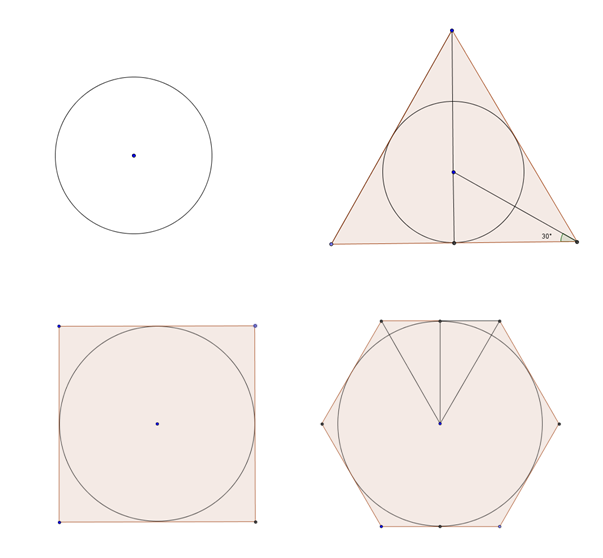
\includegraphics[width=10cm]{1munten}
\caption{De dienbladen voor 1 munt}
\label{1munt}
\end{figure}

\begin{itemize}
	\item \textbf{Cirkelvormig dienblad:} \\
	Wanneer we slechts 1 munt hebben, is een cirkelvormig dienblad het effici�nst, omdat er dan geen vrije ruimte meer overblijft. E�n munt neemt dus 100\% van de oppervlakte van het cirkelvormig dienblad in. We kunnen dit als volgt samenvatten:
	
	\begin{itemize}
	\item Oppervlakte dienblad = 12,5664 cm$^2$
	\item Effici�ntie = 100\%
\end{itemize}
	
	\item \textbf{Driehoekig dienblad:}\\
	Bij een driehoekig dienblad is de lengte van de basis gelijk aan $2.2.\tan(\pi/6)=4\sqrt{3}\approx 6,9282$ cm. De hoogte is $\sqrt{b^2-(\frac{b}{2})^2}= 6$ cm. Daaruit volgt dat:
	\begin{itemize}
	\item Oppervlakte dienblad = $20,7846$ cm$^2$
	\item Effici�ntie = 60,46 \%
\end{itemize}	

	\item \textbf{Rechthoekig dienblad:}\\
	De oppervlakte van de meest compacte rechthoek voor 1 jeton is niet moeilijk te vinden. Aangezien we zien dat de lengte en de breedte beide gelijk zijn aan de diamter van de munt, weten we dat:
	
	\begin{itemize}
	\item Oppervlakte dienblad = $16$ cm$^2$
	\item Effici�ntie = 78,54\%
\end{itemize}
	
	\item \textbf{Zeshoekig dienblad:}\\
	Voor de oppervlakte van de gelijkzijdige zeshoek te berekenen, moeten we de straal van deze zeshoek berekenen (of zijde, die daaraan gelijk is). Deze is gelijk aan de straal van de jeton gedeeld door $\cos(\pi/6)$. Dus in de formule $\frac{3}{2}.z^2.\sqrt{3}$ is $z=2,3094$ en vinden we dus dat de oppervlakte van de zeshoek gelijk is aan 13,8564 cm$^2$. 
	
	\begin{itemize}
	\item Oppervlakte dienblad = 13,8564 cm$^2$
	\item Effici�ntie = 90,69\%
\end{itemize}
\end{itemize}

\end{vb}

\begin{vb}[Dienbladen met 2 munten]

\begin{figure}[h]
\centering
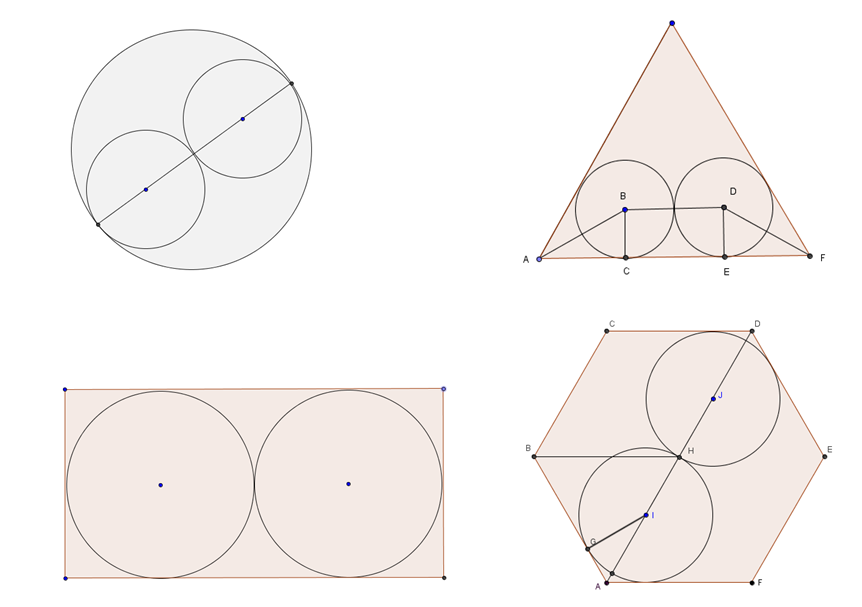
\includegraphics[width=10cm]{2munten}
\caption{De dienbladen voor 2 munten}
\label{2munt}
\end{figure}


\begin{itemize}
\item[] 
\begin{itemize}
	\item Oppervlakte munten =  $8\pi\approx 25,1327$ cm$^2$
\end{itemize}
\end{itemize}
\begin{itemize}
  \item \textbf{Cirkelvormig dienblad:}\\
  Om de oppervlakte te berekenen hebben we de straal van de grote cirkel nodig. Die is twee maal de straal van de munten en dit is $4$ cm.  Hieruit volgt
  \begin{itemize}
	  \item Oppervlakte dienblad = $16\pi\approx 50,2655$ cm$^2$
	  \item Effici�ntie = 50\%
  \end{itemize}
  
	\item \textbf{Driehoekig dienblad:}\\
	De configuratie op de figuur geeft dezelfde als de configuratie met een munt in de rakende in de tophoek (je kan dit inzien door de figuur te draaien).
	De grootte van basis van de driehoek is gelijk aan twee keer de grootte van de projectie van het lijnstuk $[AB]$ (op de figuur), dus twee keer de grootte van $[AC]$, en de lengte van $[BD]$. Deze laatste is twee keer de straal van de jetons, dus gelijk aan 4 cm, omdat de cirkels elkaar juist raken. De grootte van $[AC]$ heeft grootte $2\sqrt{3}$ cm zoals bij de berekeningen van het voorbeeld met 1 munt. De grootte van de basis is dus gelijk aan 4+4$\sqrt{3}\approx 10,9282$ cm. Met deze basis weten we dat de hoogte van de driehoek 9,4641 cm is. Hieruit vinden we :
	
	\begin{itemize}
	\item Oppervlakte dienblad = 51,7128 cm$^2$.
	\item Effici�ntie = 48,60\%
\end{itemize}
	
	
	\item \textbf{Rechthoekig dienblad:}\\
	De rechthoek die de 2 munten omvat heeft een lengte van 4 keer de straal van de munten en de breedte is gewoon de diameter. Zo vinden we dus :
	\begin{itemize}
	\item Oppervlakte dienblad = 32 cm$^2$
	\item Effici�ntie = 78,54\%
\end{itemize}
	
	\item \textbf{Zeshoekig dienblad:}\\
	\todo{Een oplossing duizend keer makkelijk dan die in het bestand van Jordy, maar wel met dezelfde uikomst. Maar controleer het toch nog maar eens goed.}
	Om de oppervlakte van de zeshoek te weten willen we graag de straal (= de zijde) van de zeshoek. Deze kunnen we vinden door het berekenen van de lengte va $[AI]$ en $[IH]$. Dit laatste is gewoon de straal van 2 cm. $|AI|$ kunnen we vinden als we $I$ loodrecht gaan projecteren op $AB$. $|GI|$ is dan ook de straal en we weten dat in deze driehoek de hoek $G\hat{A}I=60�$. Hieruit halen we dat $|AI|=\frac{|GI|}{\sin(60�)}=2,3094$ cm en dus de grootte van de straal is 4,3094 cm.
	\begin{itemize}
	\item Oppervlakte dienblad = 48,2487 cm$^2$
	\item Effici�ntie = 52,09\%
\end{itemize}
\end{itemize}


\end{vb}


\begin{vb}[Dienblad met 3 munten]


\begin{figure}[h]
\centering
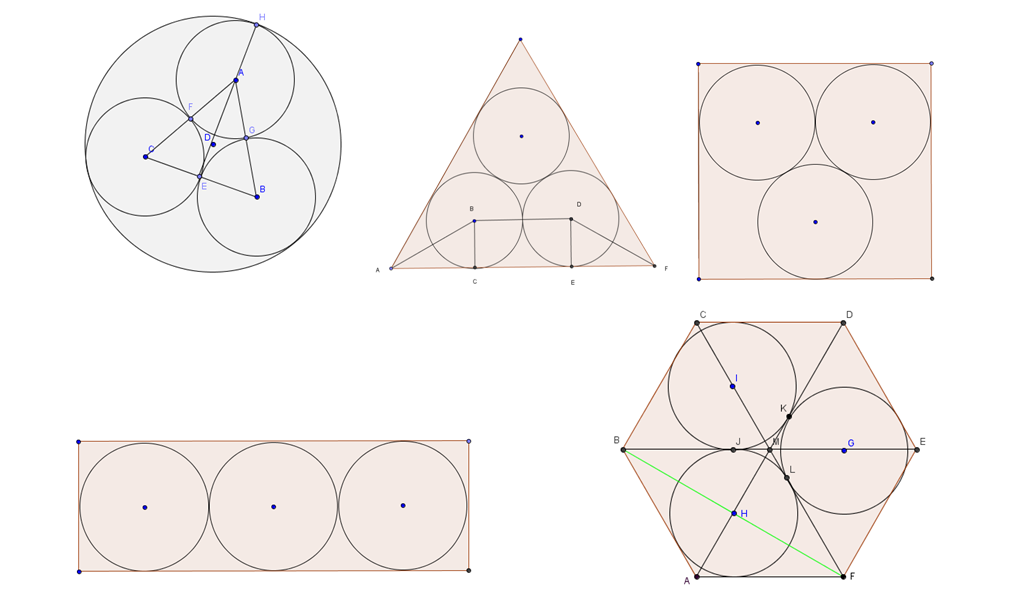
\includegraphics[width=18cm]{3munten}
\caption{De dienbladen voor 3 munten}
\label{3munt}
\end{figure}


\begin{itemize}
	\item 
	\begin{itemize}
	\item Oppervlakte 3 munten= $12\pi\approx 37,70$ cm$^2$
\end{itemize}
\end{itemize}


\begin{itemize}
  \item \textbf{Cirkelvormig dienblad:}\\
  De straal van de cirkel is deze keer gelijk aan de som van de lengtes van twee lijnstukken, $|HA|$ en $|AD|$. De lengte van $[HA]$ is gelijk aan de straal van de munten. De lengte van $[AD]$ vinden we in de driehoek $ABC$. Doordat deze driehoek gelijkzijdig is, geldt dat de hoogtelijnen elkaar in 1 punt snijden, het hoogtepunt. En dit punt verdeelt elke hoogtelijn van de driehoek in twee delen waarvan het ene deel twee keer zo groot is als het ander. Met andere woorden, de lengte van $[AD]$ is twee keer de lengte van $[DE]$. Doordat $|AE|=\sqrt{|AB|^2-|BE|^2}=\sqrt{16-4}=\sqrt{12}\approx 3,4641$ cm, is de lengte van $[AD]$ gelijk aan 2,3094cm. Hieruit volgt dat de straal van het cirkelvormig dienblad een lengte van 4,3094 cm heeft. Het is ook niet verwonderlijk dat dit dezelfde straal geeft als de zeshoek in vorig voorbeeld. \\
 We vinden dus volgende resultaten:
   
  
  \begin{itemize}
	\item Oppervlakte dienblad = 58,36 cm$^2$.
	\item Effici�ntie= 64,62 \%
\end{itemize}
     
	\item \textbf{Driehoekig dienblad:}\\
	Aangezien het driehoekige dienblad bij drie munten hetzelfde is als dat bij twee munten hoeven we de berekeningen voor de oppervlakte van het dienblad niet opnieuw te doen. We weten dus dat:
	
	\begin{itemize}
	\item Oppervlakte dienblad = 14,80 cm$^2$.
	\item Compactheid dienblad = 72,90 \%
\end{itemize}
	
	\item \textbf{Rechthoekig dienblad:}\\
	Zoals je ziet zijn er twee figuren van rechthoeken opgenomen in dit voorbeeld. Hierin is duidelijk te zien welke rechthoekig dienblad het meest effici�nt is (namelijk die waar de drie glazen naast elkaar staan). Deze effici�ntie kunnen we eigenlijk al overnemen van de vorige voorbeelden, omdat je als het waren 3 vierkante dienbladen van 1 munt naast elkaar plakt. Als we echter toch even de eenvoudige berekeningen hernemen, bekomen we dat de lengte van het rechthoekig dienblad 6 keer de straal is van de munten en de breedte de diameter. Voor zo een rechthoek geldt dus:
	
	\begin{itemize}
	\item Oppervlakte dienblad = 45 cm$^2$
	\item Effici�ntie = 78,54\%
\end{itemize} 
	
	
	\item \textbf{Zeshoekig dienblad:}\\
	Om de straal van de zeshoek $ABCDEF$ te verkrijgen berekenen we eerst de lengte van het groene lijnstuk. Dit groene lijnstuk $[FB]$ is in twee gelijke delen verdeeld ($|FH|$ en $|HB|$). Deze delen hebben een lengte die gelijk is aan de hoogte van de meest compacte gelijkzijdige driehoek bij 1 munt min 1 keer de straal van de munt (Dit kan je zien door bijvoorbeeld de driehoek die vertrekt in top B te beschouwen met de meest linkse cirkel). Dus $|HB|=|FH|=4$cm. De lengte van het groene lijnstuk heeft dus een lengte van 8 cm. De lengte van de straal in de zeshoek kunnen we nu eenvoudig verkrijgen in de rechthoekige driehoek $AFH$. Daarin geldt namelijk $\cos(30�)=\frac{4}{z}$ met $z$ de zijde van de zeshoek. Deze $z$ is dus gelijk aan 4,6188 cm. Zo kunnen we besluiten dat 
	\begin{itemize}
	\item Oppervlakte dienblad = 55,4256 cm$^2$
	\item Effici�ntie = 68,02\%
\end{itemize}
	
	
\end{itemize}
\end{vb}

\begin{vb}[Dienblad met 11 munten]

\begin{itemize}
  \item \textbf{Rechthoekig dienblad:}\\
  Om de oppervlakte te berekenen 
   \begin{itemize}
	\item Oppervlakte dienblad = 
\end{itemize}
  
\end{itemize}
\end{vb}



\subsubsection{Conclusie}

Als we alle gegevens in de overzichtstabel hebben gezet, zouden we (ongeveer) volgend resultaat moeten krijgen, waarbij de grootste waarden in een kleurtje staan \todo{Hoe doe je dit in LaTeX om in een tabel een vakje te kleuren??}:


\begin{table}[h]
\centering
\begin{tabular}{l||c|c|c|c}
Aantal / vorm & cirkelvormig & driehoekig & rechthoekig& zeshoekig\\\hline\hline
1& \cellcolor[rgb]{1,0,0} 100\% & 60,46\%&90,69\% & 78,54\%\\\hline
2& 50\%& 48,60\% & 52,09\% & 78,54\%\\\hline
3&64,62\%& 72,90\% & 68,02\% & 78,54\%\\\hline
4&&&&\\\hline
5&68,52\%& 65,11\% & 62,14\% & 78,54\%\\\hline
6&&&&\\\hline
7&77,78\%& 63,71\% & 85,05\% & 78,54\%\\\hline
8&&&&\\\hline
9&&&&\\\hline
10&&&&\\\hline
11& 71,45\%& 64,40\% & 64,79 \% & 79,06\%\\\hline
12&&&&\\\hline
13&72,45\%& 71,77 \% & 70,20 \% & 78,54\%\\\hline
...&&&&
\end{tabular}
\caption{De effici�ntie van de dienbladen bij een bepaalde hoeveelheid glazen of blikjes}
\label{}
\end{table}


Zoals we in de overzichtslijst kunnen zien, zijn de rechthoekige dienbladen gemiddeld genomen het effici�ntst. Op de tweede plaats komen de cirkelvormige en de zeshoekige dienbladen. In de realiteit merken we dat men in de restaurants en in de caf�s bijna altijd cirkelvormige en rechthoekige dienbladen gebruikt. Waarschijnlijk zullen de uitbaters de compactheden van hun dienbladen niet berekend hebben, maar de fabrikanten van de dienbladen wel. Het is dus ook logisch dat de uitbaters dienbladen gebruiken die het meest effici�nt zijn. De rechthoekige dienbladen hebben inderdaad de grootste effici�ntie. Dit komt echter voornamelijk omdat we gewerkt hebben met lange smalle dienbladen waarbij alle glazen achter elkaar staan. Hadden we echter gewerkt met vierkanten, zouden we waarschijnlijk niet zo een hoge effici�ntie hebben gehad. Zeshoekige dienbladen zal men in de praktijk minder gebruiken, want ondanks dat er wel zeshoekige dienbladen zijn die een hoge compactheid hebben, zijn er ook veel zeshoekige dienbladen die een relatief kleine compactheid hebben. De cirkelvormige dienbladen zijn dan weer beter en misschien wel het best van alle dienbladen. Want ondanks dat zij nooit echt de hoogste compactheid hebben, zijn ze toch redelijk effici�nt te noemen. De waardne van de effici�nties kennen immers geen grote pieken en dalen en blijven gemiddeld genomen rond de 70\% draaien, wat een mooie waarde is. 
Onze laatste vaststelling is dat de driehoekige dienbladen nooit een grote effici�ntie hebben met het logische gevolg dat we dus ook zo goed als geen driehoekige dienbladen tegenkomen in de dagelijkse wereld. 

\newpage
\section{Driedimensionale stapelproblemen}
In de voorbije lessen, hielden we ons bezig om cirkels op een zo optimaal mogelijke manier te stapelen in een driehoek, rechthoek, cirkel ...
Als we dit probleem veralgemenen naar het driedimensionaalgeval, dan krijgen we het zogenaamde probleem van Kepler, waarbij we dus zoeken naar de dichtste bolstapeling.

\subsection{Kanonskogels stapelen}

\begin{wrapfigure}[10]{r}{0.3\textwidth}
  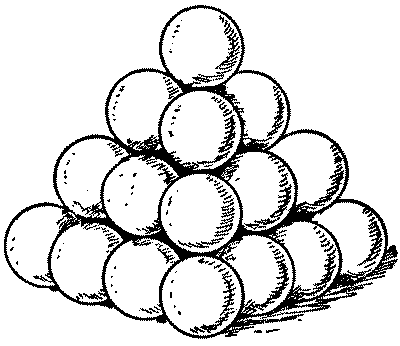
\includegraphics[width=0.3\textwidth]{cannonballs}
\end{wrapfigure}

Ondanks dat het bolstapelprobleem ook het probleem van Kepler genoemd wordt, ontstond het niet bij Kepler, maar bij de Engelse admiraal Sir Walter Raleigh. Wanneer deze Engelse admiraal naar buiten keek vanuit zijn admiraliteitsgebouw, zag hij steeds piramidevormige stapels bestaande uit kanonskogels.  Deze stapels intrigeerden hem zodanig, dat hij zich op een welbepaalde dag afvroeg hoeveel kanonskogels er in zo'n stapel aanwezig waren. Daarom ging hij ten rade bij zijn wetenschappelijk adviseur, Thomas Harriot, om dit  raadsel voor hem op te lossen. 

Voor deze les gaan we ons wat inleven in de rol van Sir Walter Raleigh. Alleen zullen we nu het niet direct vragen aan Thomas Harriot, maar het zelf onderzoeken.

Bolvormige kanonskogels kun je op verschillende manieren als een piramide op elkaar stapelen. Je kunt bijvoorbeeld beginnen om de eerste laag kogels in een vierkant patroon te leggen, maar ook volgens gelijkzijdige driehoeken is het mogelijk, net als bij de jetons in het vlak of de blikjes/glazen op het dienblad. 
Omdat we toevallig niet voldoende kanonskogels bij de hand hebben, kunnen we knikkers gebruiken om dit uit te proberen (ook tafeltennisballetjes of sinaasappelen zijn geschikt).

\task{Ga op zoek naar de formule voor het aantal kanonskogels in een (regelmatige) piramide met vierkant en driehoekig grondvlak (ook voor cirkelvormig en zeshoekig grondvlak zou je dit kunnen uitproberen) met $n$ lagen. \\
Test dit eerst uit door het zelf uit te testen met knikkers voor 1,2, 3 ... lagen. Vul dit in onderstaande tabel in en probeer hieruit zelf tot een formule te komen. Ga dan eens na hoeveel kogels je moet hebben voor 100 lagen.}

\begin{table}[h]
\centering
\begin{tabular}{l|c|c|c|c|c|c}
Aantal lagen: &&&&&&\\\hline\hline
Driehoek: &&&&&& \\\hline
Vierkant: &&&&&& \\
\end{tabular}
\caption{Aantal knikkers voor verschillende piramides met $n=1,...,6$ lagen}
\end{table}



\answer{Het is nu de bedoeling dat de leerlingen zelf de formule gaan zoeken en vinden door dit uit te testen voor verschillende vormen van grondvlakken en voor verschillende lagen ($n = 1, 2, ... , 6 , ... , 100$). Hiervoor kunnen ze dus gebruik maken van knikkers, waarbij je best ook zorgt voor een ruwe ondergrond of een soort omkadering voor het grondvlak. Ook andere bolvormige voorwerpen kunnen gebruikt worden.
De leerlingen zullen algauw gevonden hebben hoeveel knikkers ze moeten gebruiken voor de verschillende rijen en de tabel als volgt hebben ingevuld.
\begin{table}
\centering
\begin{tabular}{l|c|c|c|c|c|c}
Aantal lagen: &1&2&3&4&5&6\\\hline\hline
Driehoek: &1&4&10&20&35&56 \\\hline
Vierkant: &1&5&14&30&55&91 \\
\end{tabular}
\caption{Aantal knikkers voor verschillende piramides met $n=1,..,6$ lagen}
\end{table}
Ook de formule met de sommen moet zeker mogelijk zijn om gevonden te worden.
\begin{itemize}
	\item Formule bij piramide met driehoekig grondvlak:
	 $$d(n)= \frac{1.2}{2} + \frac{2.3}{2}+\frac{3.4}{2} + \cdots + \frac{n(n+1)}{2}$$
	\item Formule bij piramide mert vierkant grondvlak: \[v(n)=1^2 + 2^2 + \cdots + n^2\]
\end{itemize}
}

\task{Test met de knikkers als je volgende vragen een positief antwoord kunnen hebben of vermoedelijk fout zijn...
\begin{itemize}
	\item Kan je van een driehoekige stapel van een bepaalde hoogte een vierkante piramide maken, zonder dat je kogels overhoudt?
	\item Kan je van twee stapels knikkers in vierkante piramides een nieuwe vierkante piramide maken? 
	\item Kan je van twee stapels knikkers in driehoekige piramides een nieuwe driehoekige piramide maken?
	\item Kan je van twee stapels knikkers in driehoekige piramides een nieuwe vierkante piramide maken?
	\item Kan je van een combinatie van een driehoekige en vierkante piramides een andere combinatie van een driehoekige en vierkante piramide maken?\\
Opmerking: piramides van ��n verdiep hoog worden niet meegerekend.
\end{itemize}
}

\teacher{
Na deze testfase is het de bedoeling dat we dit klassikaal overlopen en de antwoorden verklaren.}


\subsubsection{Het aantal kanonskogels bij een piramide met vierkant grondvlak}

We zullen beginnen met de vierkante stapeling.
Om bijvoorbeeld een stapel van vier lagen hoog te maken begin je om 16 kogels netjes in een 4 bij 4 vierkant te leggen. Vervolgens leg je daarop een laag van 9 kogels in een 3 bij 3 vierkant, dan een laag met $2\times2=4$ kogels, en ten slotte is er nog plaats voor ��n kogel als top van de piramide. Voor een 'vierkante' stapel van vier lagen hoog heb je dus $16+9+4+1=30$ kogels nodig.
Als je kijkt naar de antwoorden die je in de tabel gevonden hebt, zijn dat eigenlijk telkens de eerste $n$ kwadraten en dus verkrijg je volgende formule:

\[v(n)=1^2 + 2^2 + \cdots + n^2.\]

\ask{Wat is het nadeel van deze formule als jij bijvoorbeeld het aantal kogels in een stapel van honderd lagen wil bepalen?}
\answer{Om het aantal kogels in een stapel van honderd lagen te bepalen moet je dus ook de eerste honderd kwadraten bij elkaar optellen. Dit is wel te doen, maar een nadeel van dit algoritme is dat de hoeveelheid werk afhangt van de hoogte van de stapel. Voor duizend lagen is het minstens tienmaal zoveel werk als voor honderd.} 

We zullen daarom nu een formule afleiden, waarmee je de som van de eerste $n$ kwadraten direct kunt uitrekenen. Het rekenwerk in een formule is vrijwel onafhankelijk van de hoogte van de piramide. Dat is het verschil met het algoritme waarin de kwadraten worden opgeteld. 

Als we het aantal kogels bij een piramide met $n$ lagen voorstellen door $v(n)$. Dan is $v(1)=1$, $v(2) = 5$ en $v(n)= 1^2 + 2^2+ \cdots +(n-1)^2 + n^2 $. 

\ask{Wat merk je op als je verschillen tussen twee opeenvolgende $v(i)$'s bekijkt?}
\answer{We merken op dat de verschillen tussen twee opeenvolgende $v(i)$'s steeds een kwadraat is, namelijk $v(n)-v(n-1)=n^2$.}
We willen proberen om nu een eenvoudigere formule te vinden voor $v(n)$, een functie die afhangt van $n$, waarbij we dus ook rekening houden met bovenstaande opmerking. Omdat er in de formule 
\[v(n) = 1^2 + 2^2+ \cdots +(n-1)^2 + n^2 \]
enkel kwadraten in voorkomen, kunnen we eens proberen als een kwadratische functie zou kunnen. 

Stel bijvoorbeeld
$$ v(n) = an^2+bn+c.$$
Als dit klopt, dan moet er gelden dat 
\begin{align*}
n^2&=v(n) - v(n-1)=(an^2+bn+c) - (a(n-1)^2+b(n-1)+c)\\
&= (an^2+bn+c) - (an^2-2an)  - (bn-b)-c=2an+(-a+b).
\end{align*}

\ask{Is het mogelijk om hieruit een formule voor $v(n)$ te vinden? Waarom wel/niet?}
\answer{
Je ziet dat helaas de term $an^2$ wegvalt. Er blijft geen kwadratische term over, dus we krijgen het zo nooit voor elkaar om voor elke $n$ waarde $n^2$ uit te komen
In het rechterlid staat iets lineair, in het linkerlid iets kwadratisch. We kunnen nooit $a, b$ en $c$ vinden die dit in orde maken.We zien hier ook de volgende eigenschap van rijen opduiken: De verschilrij van een kwadratische rij is een lineaire rij.}

Aangezien dit niet werkt, is een volgend idee om voor $v(n)$ een derdegraadsfunctie in $n$ te nemen: \[v(n)=an^3+bn^2+cn+d.\]

Dan valt waarschijnlijk de derdegraadsterm weer weg, maar misschien hou je iets kwadratisch over. Er is nog een ander reden waarom dit niet zo'n vreemd idee is. Het aantal kanonskogels in piramide heeft iets te maken met zijn inhoud. Inhoud is iets driedimensionaal met zoiets als de lengte, breedte en hoogte, die telkens van de orde $n$ zijn, dus zal het aantal waarschijnlijk iets met de derde macht van $n$ te maken hebben. 

\task{Ga nu zelf na op analoge wijze dat deze aanpak inderdaad goed blijkt te werken en probeer via een stelsel de juiste waarden voor $a,b$ en $c$ te vinden.}
\answer{
\begin{align*}
n^2&=v(n)-v(n-1)=(an^3+bn^2+cn+d) -(a(n-1)^3+b(n-1)^2+c(n-1)+d)\\
&= (an^3+bn^2+cn+d) -[(an^3-3an^2+3an-a)+(bn^2-2bn+b)+(cn-c)+d]\\
&= 3an^2+(-3a+2b)n+(a-b+c).  
\end{align*}
In deze formule staat aan de linkerkant $n^2$ en rechts een kwadratische functie in $n$. Als we op zoek zijn naar de formule moeten we er zeker voor zorgen dat de co�ffici�nten van de machten van $n$ in beide leden gelijk zijn. Zo moet dus het volgende stelsel gelden:
\[\displaystyle
   \left\{ 
  \begin{array}{l l}
	1&= 3a\\
    0&= -3a+2b \\
     0&= a-b+c\\    
  \end{array}\right.\]  
  Het oplossen van dit stelsel levert ons de waarden $a=\frac{1}{3}$, $b=\frac{1}{2}$ en $c=\frac{1}{6}$. Er geldt dus dat 
$$v(n)= 1^2 + 2^2 + \cdots + n^2= \sum_{i=1}^{n}i^2= \frac{1}{3}n^3+\frac{1}{2}n^2+\frac{1}{6}n + d.$$ En omdat $v(1)=1=1+d$ is $d=0$.
}

 
We verkrijgen dus het volgende resultaat:
\[ v(n)= 1^2 + 2^2 + \cdots + n^2= \frac{1}{3}n^3+\frac{1}{2}n^2+\frac{1}{6}n .\]
Met deze formule kun je dus eenvoudig uitrekenen voor hoeveel kanonskogels er in een stapel van een bepaalde hoogte gaan. Voor een hoogte van $n=4$ lagen krijg je inderdaad 30 kogels, zoals we al eerder zagen. Voor 100 lagen zijn maar liefst 338350 kanonskogels nodig.


De formule voor het aantal kanonskogels bij een piramide van $n$ lagen hoog met vierkant grondvlak is eigenlijk de som van de eerste $n$ kwadraten. 
Meestal wordt de formule geschreven als \[\sum_{i=1}^{n}i^2=\frac{n(n+1)(2n+1)}{6}. \]

\task{ Reken dit even uit om te zien dat dit inderdaad overeenkomt met de formule die wij reeds vonden.}


E�n merkwaardig aspect van deze formule is dat er breuken in staan, terwijl het eindantwoord een aantal is en dus altijd een natuurlijk getal moet zijn. 
\todo{Ik vind het moeilijk om hier een vraag of opdracht van te maken, omdat dit wel niet zo makkelijk is om als 16jarige dit op te lossen. Anders gewoon dit zoals ervoor als opmerking schrijven.}

Dat dit toch altijd goed uitkomt, ondanks de breuken, kun je zien door de formule te schrijven zoals in de vorige opmerking, namelijk $v(n)=\frac{n(n+1)(2n+1)}{6}$.\\ 
Deze vorm zal het ons eenvoudiger maken om te controleren dat de formule effectief een geheel getal is. We willen aantonen dat $n(n+1)(2n+1)$ deelbaar is door 6, of dus deelbaar is door 2 en door 3.\\
Dat $n(n+1)(2n+1)$ deelbaar is door 2 volgt uit het feit dat elk getal $n$ even is, of anders is $n+1$ het wel. Dit betekent dat $n(n+1)$ altijd deelbaar is door 2. 
Als je nu nog kan aantonen dat $n(n+1)(2n+1)$ altijd deelbaar is door 3, dan weten we dat de formule steeds te schrijven is als een geheel getal.
Stel dat $n$ en $n+1$ niet deelbaar zijn door 3, waarbij de resten bij deling door 3 steeds 1 en 2 moeten zijn. Aangezien $2n+1=n+(n+1)$ geeft dit dus 3 (dus 0) als rest bij deling door 3. Hieruit volgt dat $v(n)$ weldegelijk steeds een natuurlijk getal geeft. 


\subsubsection{Het aantal kanonskogels bij een piramide met driehoekig grondvlak}

Vervolgens kijken we eens naar een piramide met driehoekig grondvlak, meerbepaald een gelijkzijdige (of regelmatige) driehoek als grondvlak.

Bij het experimenteren daarnet heb je zeker gevonden dat je bij een stapel van vier hoog $10+6+3+1=20$ kogels nodig hebben. Merken we op dat 1, 3, 6 en 10 driehoeksgetallen zijn, ze zijn namelijk van de vorm $\frac{n(n+1)}{2}$. Dit komt omdat je per laag een driehoek bekomt met op de top 1 bol, daaronder 2, daaronder 3 enzovoort tot ten slotte $n$ bollen als we ons bevinden op de grondlaag, en de som van de natuurlijke getallen tot en met $n$ is $\frac{n(n+1)}{2}$

Als je nu dezelfde werkwijze als hierboven toepast, bekom je dat 
\begin{align*}
d(n) &= \frac{1.2}{2} + \frac{2.3}{2}+\frac{3.4}{2} + \cdots + \frac{n(n+1)}{2}=\sum_{i=1}^{n}\frac{i(i+1)}{2}\\
&=\frac{1}{6}n^3 + \frac{1}{2}n^2+\frac{1}{3}n.
\end{align*}

Met deze formule kun je dus eenvoudig uitrekenen voor hoeveel kanonskogels er in een stapel van een bepaalde hoogte gaan. Voor een hoogte van $n=4$ lagen krijg je inderdaad 20 kogels, zoals we al eerder zagen. 

\ask{Hoeveel kanonskogels heb je nodig voor 100 lagen?}

\answer{Voor 100 lagen hebben we deze keer 171700 kanonskogels nodig.}

\task{
Ga op analoge wijze als bij de piramide met vierkant grondvlak tewerk en ga na dat dit effectief de juiste formule is.}

\answer{
Als we het aantal kogels bij een driehoekige piramide met $n$ lagen voorstellen door $d(n)$. Dan is $d(1)=1$, $d(2) = 4$ en $d(n)= \frac{1.2}{2} + \frac{2.3}{2}+\frac{3.4}{2} + \cdots + \frac{n(n+1)}{2}$. We merken op dat de verschillen tussen twee opeenvolgende $v(i)$'s steeds een driehoeksgetal is, namelijk $d(n)-d(n-1)=\frac{n(n+1)}{2}$.
We willen proberen om nu een eenvoudigere formule te vinden voor $d(n)$, een functie die afhangt van $n$. Omdat er in de formule
enkel kwadraten in voorkomen, kunnen we eens proberen als een kwadratische functie zou kunnen. Analoog als bij het geval met de vierkante piramide zie je dat de term $an^2$ wegvalt. Er blijft geen kwadratische term over.\\
Een volgend idee is om voor $d(n)$ een derdegraadsfunctie in $n$ te nemen: $$d(n)=an^3+bn^2+cn+d.$$ Ook hier blijkt dit opnieuw te werken.
\begin{align*}
\frac{n(n+1)}{2}&=d(n)-d(n-1)=(an^3+bn^2+cn+d) -(a(n-1)^3+b(n-1)^2+c(n-1)+d)\\
&= (an^3+bn^2+cn+d) -[(an^3-3an^2+3an-a)+(bn^2-2bn+b)+(cn-c)+d]\\
&= 3an^2+(-3a+2b)n+(a-b+c).  
\end{align*}
In het linkerlid staat $\frac{n(n+1)}{2}= \frac{1}{2}n^2+\frac{1}{2}n$. Gelijkstellen van de co�ffici�nten van de machten van $n$ in beide leden geeft ons opnieuw een stelsel:
\[\displaystyle
   \left\{ 
  \begin{array}{l l}
	\frac{1}{2}&= 3a\\
     \frac{1}{2}&= -3a+2b \\
     0&= a-b+c\\    
  \end{array}\right.
  \]  
Het oplossen van dit stelsel levert ons de waarden $a=\frac{1}{6}$, $b=\frac{1}{2}$ en $c=\frac{1}{3}$. Er geldt dus dat 
\begin{align*}
d(n) &= \frac{1.2}{2} + \frac{2.3}{2}+\frac{3.4}{2} + \cdots + \frac{n(n+1)}{2}=\sum_{i=1}^{n}\frac{i(i+1)}{2}\\
&=\frac{1}{6}n^3 + \frac{1}{2}n^2+\frac{1}{3}n+d.
\end{align*}
Omdat $d(1)=1=1+d$ is $d=0$ en krijgen we het gezochte resultaat.
}

\subsubsection{Combinaties van bepaalde piramides}
We weten nu hoeveel kogels er nodig zijn om een \textquoteleft driehoekige' of \textquoteleft vierkante' piramide van kogels te stapelen. We gaan nu op zoek naar de antwoorden op de vragen over het combineren van bepaalde stapels knikkers in de vorm van piramides.

\ask{Is het nu mogelijk om van een driehoekige stapel van een bepaalde hoogte een vierkante piramide te maken, zonder dat je kogels overhoudt?} 

Als je kijkt naar het lijstje, dat we vroeger reeds maakten, met de aantallen die nodig zijn voor een driehoekige, vierkante en zeshoekige piramide, dan zie je dat dit nooit lijkt te kunnen, behalve natuurlijk voor een stapel van ��n kogel hoog.
De aantallen in de driehoekige stapel lijken niet voor te komen in de rij van de vierkante piramides. De tabel kun je nog veel groter maken, maar als er nog steeds geen gelijke getallen voorkomen weet je niet zeker of het nooit gebeurt. Misschien gebeurt het namelijk toch een keer voor een heel er grote stapel. Twee Nederlandse wiskundigen (Frits Beukers en Jaap Top) hebben in 1982 bewezen dat het inderdaad nooit gebeurt, maar het bewijs is te moeilijk om er hier op in te gaan.

\ask{Kan je van twee stapels knikkers in driehoekige piramides een nieuwe vierkante piramide maken?}

\answer{Dit is inderdaad mogelijk.}

\ask{Kan je hiervan een voorbeeld geven?}

\answer{Een driehoekige piramide van 3 lagen en een van 4 lagen bestaan samen bijvoorbeeld uit $10+20=30$ kogels, precies genoeg voor een vierkante piramide van 4 lagen hoog.}

Aan de hand van de verkregen formules kan je aantonen dat dit altijd waar is.

\task{Als je het aantal kogels in een vierkante stapel nog steeds stelt als $v(n)= \frac{1}{3}n^3+\frac{1}{2}n^2+\frac{1}{6}n $ en in een driehoekige stapel als $d(n) =\frac{1}{6}n^3 + \frac{1}{2}n^2+\frac{1}{3}n$, controleer dan dat effectief \[d(n-1)-d(n)=v(n).\]}

\answer{
Als we dit met de formules uitschrijven, krijgen we inderdaad
\begin{align*} 
d(n-1) + d(n)&= \frac{1}{6}(n-1)^3 + \frac{1}{2}(n-1)^2+\frac{1}{3}(n-1)+ \frac{1}{6}n^3 + \frac{1}{2}n^2+\frac{1}{3}n\\
&= (\frac{1}{6}n^3 - \frac{1}{2}n^2+\frac{1}{2}n-\frac{1}{6})+(\frac{1}{2}n^2-n+\frac{1}{2})+(\frac{1}{3}n-\frac{1}{3})+(\frac{1}{6}n^3 + \frac{1}{2}n^2+\frac{1}{3}n)\\
&= \frac{1}{3}n^3 + \frac{1}{2}n^2+\frac{1}{6}n= v(n). 
\end{align*}}

Ten slotte kunnen we ook onderstaande vraag positief beantwoorden.

\ask{Kan je van een combinatie van een driehoekige en vierkante piramides een andere combinatie van een driehoekige en vierkante piramide maken?}

\task{Geef een voorbeeld van zo een combinatie.}

\answer{Een vierkante piramide van 5 lagen en een driehoekige piramide van 4 lagen bevatten samen 65 kogels. Een vierkante piramide van 5 lagen en een driehoekige piramide van 3 lagen bevatten samen ook 65 kogels.}  

\task{Hier zit een algemeen patroon achter. Schrijf deze formule op en probeer deze te bewijzen a.d.h.v. de formule uit vorige opdracht.}

\answer{Uit $v(n)=d(n-1)+d(n)$ halen we dat 
\[ v(n)+d(n+1)=d(n-1) + d(n) + d(n+1) = d(n-1) + v(n+1).\]}

%Snifsnif, dit moet weg :s ...
%\subsection{De hoogte van een stapel kanonskogels}
%We hebben het tot nu toe gehad over het aantal bollen in een piramide, maar hoe zit het met de hoogte? Hoe hoog is bijvoorbeeld een driehoekige piramide van 4 lagen knikkers? Is deze dezelfde als een piramide met een vierkant grondvlak?

%Voor het gemak noemen we de straal van de bollen of kanonskogels of knikkers $r$ en $n$ is opnieuw het aantal lagen. Om de hoogte van de stapel te bepalen is het handig om je te verplaatsen in de positie van de middelpunten van de bollen. 
%Je weet dat de hoogte van de grond tot het middelpunt van de bollen op de onderste laag $r$ is. Ook de hoogte van het bovenste middelpunt tot de top van de piramide is $r$. Als we nu de hoogte weten tussen de middelpunten van twee opeenvolgende lagen, dan hebben we de hoogte gevonden. Het is namelijk zo dat deze hoogtes $h$ dezelfde zijn. De hoogte van de piramide is dan $2r+h$.

%Het komt er nu dus op neer bij de verschillende stapels te zoeken wat de hoogte nu juist is.

%\subsubsection{De hoogte van een stapel met vierkant grondvlak}

%Om de hoogte te bepalen tussen twee opeenvolgende lagen van middelpunt, is het handig om te kijken naar de piramide van 2 lagen. In ons geval is dat dus een piramide van 5 bollen. Kijken we nu naar de middelpunten van deze bollen, dan zien we dat deze opnieuw een piramide vormen. Dit komt omdat de bovenste bol raakt aan de andere vier bollen en daardoor is de afstand van twee middelpunten steeds $2r$. Als we de hoogte weten van deze piramide, dan hebben we het gevonden. 

%\todo{Hier zouden allemaal mooie figuren moeten komen het het aanschouwelijk te maken.
%We kunnen ook gebruikmaken van isomobollen en satestokken die dan de bollen verbinden.}

%De hoogte van de kleine piramide vinden we door twee keer de stelling van pythagoras toe te passen. We bekomen $h=\sqrt{2}r$ als hoogteverschil tussen twee middelpunten. Op die manier vinden we de volgende hoogte van een stapel met vierkant grondvlak en $n$ lagen van bollen met straal $r$:
%$$ r(\sqrt{2}(n-1)+2).$$ 


%\subsubsection{De hoogte van een stapel met driehoekig grondvlak}
%Zo ook kunnen we nu de hoogte berekenen van een stapel met een regelmatige driehoek als grondvlak. In figuur %\ref{tetra} 
%zie je hoe de middelpunten van de bollen een stapel van tetra�ders (regelmatige viervlakken) vormen. Dit komt omdat een bol raakt aan de drie bollen onder zich. Het verbinden van het middelpunt met de 3 andere middelpunten geeft inderdaad een viervlak met zijde $2r$. 
%Op de figuur zien we dat we voor de hoogte van de stapel eerst $r$ omhoog moeten naar een middelpunt van de onderste laag, vervolgens 3 keer de hoogte van een tetra�der en ten slotten nog ��n straal omhoog en we zitten boven op de bovenste bal. De hoogte van de stapel met vier lagen ballen is dus $2r+3h$ waarbij $h$ de hoogte van een viervlak is. Voor $n$ lagen met bollen moeten we $n-1$ lagen tetra�ders omhoog.

%\begin{figure}[h]
%\includegraphics[width=\columnwidth]{tetra}
%\caption{Twintig bollen in een driehoekige piramide en tien tetra�ders gevormd door de middelpunten}
%\label{tetra}
%\end{figure}

%Nu moeten we dus enkel nog op zoek gaan naar de hoogte van zo een tetra�der.
%Beschouw figuur %\label{tetra2}
%De hoogte $h$ van de tetra�der is de lengte van z'n hoogtelijn $TP$. Dat is de lijn die je krijgt door de tetra�der op de tafel te zetten en vanuit het hoogste punt een lijn loodrecht naar beneden te trekken. Het onderste punt $P$ ligt precies midden in de onderste gelijkzijdige driehoek, even ver van alledrie de hoekpunten af. De driehoek $\Delta HMP$ heeft hoeken $30\degree$, $60\degree$ en $90\degree$. Aangezien $r= |HM|= |HP|. \cos(30\degree)=r.\frac{\sqrt{3}}{2}$ vinden we dat $$ |HP|=x= \frac{2}{\sqrt{3}}r.$$

%\begin{figure}[h]
%\includegraphics[width=\columnwidth]{tetra2}
%\caption{}%
%\label{tetra2}
%\end{figure}

%Pas nu de stelling van Pythagoras toe op de driehoek door het geprojecteerde punt $P$, een hoekpunt $H$ van de onderste driehoek en het topje $T$ van de tetra�der, dan
%vind je: $(2r)^2=x^2+h^2$. Samen met de formule voor $x$ vinden we dat de hoogte van een tetra�der met zijden van lengte $2r$ gegeven wordt door $$h=\frac{2}{3}r\sqrt{6}.$$

%De hoogte van een driehoekige piramide van $n$ lagen bollen met een straal van $r$ is dus: $$2r(\frac{\sqrt{6}}{3}(n-1)+1).$$


%\emph{Als de leerlingen in het begin hebben mogen uitproberen met knikkers, kan ook een vraag geweest zijn hoe hoog dat de piramide is van 5 lagen knikkers bij de piramide met een vierkant en met een driehoekig grondvlak. Dit kunnen ze nu ook als opdracht krijgen om effectief uit te rekenen en kijken hoever ze er vanaf zaten.}
%\begin{opdracht}
%Wat is de hoogte van een stapel knikkers gestapeld als een piramide met een vierkant grondvlak van 5 lagen? En hoe hoog is de stapel als het een driehoekig grondvlak zou zijn?
%\end{opdracht}

%\todo{Uitgangspunt cursus}
%\emph{Je kan de leerlingen nog verschillende van deze kleine rekenoefeningetjes geven om te checken desnoods, maar het belangrijskte is dat ze inzien dat er een verschil zit en dat ze zien dat de piramide met $n$ lagen bij een vierkante piramide hoger is dan een piramide met driehoekig grondvlak maar met evenveel lagen. Dit geeft reeds een aanwijzing dat, net zoals in het vlak, de vierkante vulling minder effici�nt is als de honingraatvulling. Dit is dan ook een mooie overgang naar het bolstapelprobleem van Kepler...}

%\todo{De volgende opdracht is een opdracht die ik gewoon overtyp van uit het Zebra-boekje. Zulke opdrachten kan je echter in veelvoud uitvinden ;) ...}
%\begin{opdracht}
%Hoeveel tennisballen met een diameter van 6,5 cm heb je nodig om een driehoekige pirmaide te maken die even hoog is als jezelf? Wegen de ballen samen meer of minder dan jij? Een tennisbal weegt 57 gram.
%\end{opdracht}


\subsection{Het bolstapelprobleem van Kepler}
\subsubsection{Het ontstaan}
\subsubsection*{Thomas Harriot}

\begin{wrapfigure}[7]{r}{3cm}
  \vspace*{-1cm}
  \begin{center}
  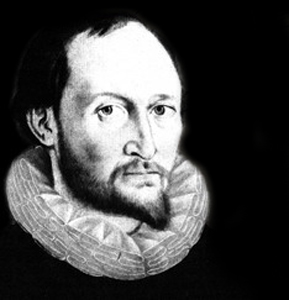
\includegraphics[width=3cm]{harriot}\\
  Thomas Harriot
  \end{center}
\end{wrapfigure}

Je kon al lezen dat Thomas Harriot (1560-1621) door Sir Walter Raleigh (1554-1618) aan het probleem van de piramidestapels werd gezet. Hij was in die tijd als amateur-astronoom bezig met het waarnemen van zonnevlekken en kometen, maar daarnaast was hij ook een bekende wiskundige en dankzij de kennis die hij als wiskundige had, kon hij het probleem van Raleigh in een wip oplossen. Maar nadat hij de oplossing geleverd had, bleef het kanonskogelprobleem in zijn hoofd rondspoken en hij raakte over dit onderwerp in correspondentie met Kepler.

Kepler, die we straks verder zullen bespreken, had al een tijdje een levendige correspondentie met Harriot over het lichtbrekingsverschijnsel. Hij was dan ook niet verbaasd toen hij een briefje kreeg van Harriot. Maar toen hij las dat het over het stapelen van bolvormige voorwerpen ging, werd zijn nieuwsgierigheid aangewakkerd. Niet veel later kwam plots de gedachte bij hem op, om aan de hand van bolstapelingen de structuur van sneeuwkristallen te verklaren. En zo verhuisde het bolstapelprobleem definitief van de gedachten van Thomas Harriot naar die van Johannes Kepler.

\subsubsection*{Johannes Kepler}

\begin{wrapfigure}[9]{l}{3cm}
  \vspace{-10mm}
  \begin{center}
  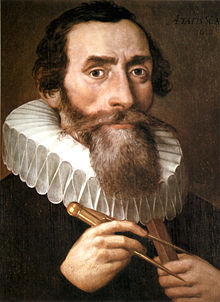
\includegraphics[width=3cm]{kepler}\\
  Johannes Kepler
  \end{center}
\end{wrapfigure}

Kepler (1571-1630) was een beroemde Duitse sterrenkundige die vooral bekendheid kreeg, toen hij aan de hand van de bewegingen van de planeten een beschrijving maakte van hun ellipsvormige banen. Vanaf 1609 onderzocht hij tien jaar lang hoe de afstand van een planeet tot de centrale ster, de omlooptijd en de omloopssnelheid van die planeet be�nvloedde. Dit zou een halve eeuw later opgenomen worden in de zwaartekrachtwetten van Newton. Maar Kepler was niet alleen een beroemde astronoom, hij leverde ook een belangrijke bijdrage tot de wiskunde.

\vspace*{5mm}

In 1611 schreef Johannes Kepler, dankzij de plotselinge inspiratie die hij kreeg door een briefje van Harriot, een boekje met de titel \textquoteleft De zeshoekige sneeuwvlok'. Daarin beschreef hij verschillende methoden om identieke bolvormige voorwerpen in drie dimensies te pakken en hieruit kwam hij tot de conclusie dat de "face-centred cubic packing" de meest effici�nte pakkingsmethode was, waarbij het minst open ruimte tussen de identieke bolvormige voorwerpen overbleef. In het citaat dat hierop volgt beschrijft Kepler zelf wat de "face-centred cubic packing" is.

\begin{quote} "Op de tweede manier wordt niet alleen ieder partikel geraakt door zijn vier buren in hetzelfde vlak, maar ook door vier in het vlak erboven en vier eronder, zodat hij in totaal door twaalf wordt geraakt, en onder druk worden bolvormige partikels rombo�daal(=ruitvormig) ... De pakking zal de dichtst mogelijke zijn, zodat met geen andere rangschikking meer partikels in hetzelfde vat kunnen worden gepakt."  
\end{quote}

Nadat Kepler echter dit vermoeden geleverd had, vond hij het niet meer nodig om hiervoor een bewijs te leveren. En hierdoor bezorgde hij de wiskundigen een probleem dat hen veel bloed, zweet en tranen zou kosten. Maar na bijna 400 jaar zwoegen, zou 'het probleem van Kepler' uiteindelijk bewezen worden. Aangezien het zo lang duurde voordat men tot een bewijs kwam, is het zeker de moeite waard om eens te kijken wat er tijdens die 400 jaren met het probleem van Kepler gebeurde. We zullen dan ook eerst een schets geven van de evolutie van het bolstapelprobleem, vooraleer het bewijs zelf aan te snijden.

\subsubsection*{Kissing number}

Maar voordat we aan de evolutie van het probleem zal beginnen, willen we eerst nog iets vertellen over het getal 12, aangezien voor dit getal een belangrijke rol is weggelegd. 
Het is niet toevallig dat bij de dichtste bolstapeling die Kepler beschrijft, elke bol geraakt wordt door 12 andere identieke bollen. Het getal twaalf is namelijk het kissing number bij drie dimensies. 

\ask{Wat wordt bedoeld met 'kissing numbers'?}

\answer{Een 'kissing number' is gedefinieerd als het aantal niet-overlappende eenheidssferen dat aan een gegeven eenheidssfeer raakt.}

Andere namen hiervoor zijn bijvoorbeeld 'Newton number' of 'contact number'

\ask{Wat is het 'Kissing number' in ��n dimensie? En in twee dimensies? Teken de situatie}

\answer{In ��n dimensie is het 'kissing number' 2, in twee dimensies 6.}
\begin{figure}[h]
  \centering
  \subfloat[]{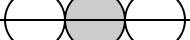
\includegraphics[width= 4 cm]{kissing1}}\qquad
  \subfloat[]{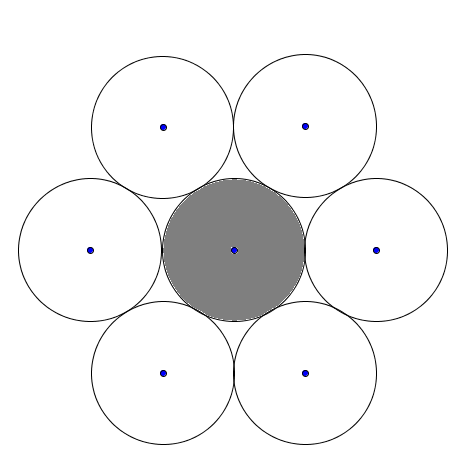
\includegraphics[width= 4 cm]{kissing2}}\qquad
  \subfloat[]{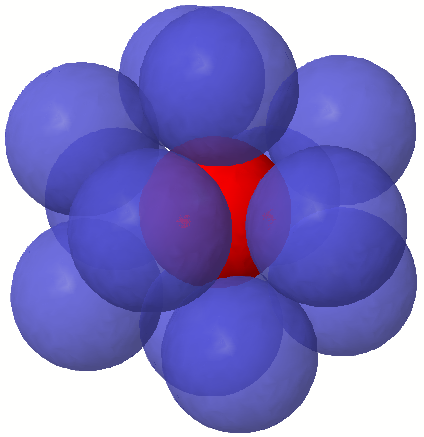
\includegraphics[width=4 cm]{kissing}}
  \caption{Illustraties van kissing number 2, 6 en 12}  
\end{figure}

In het tweedimensionale geval hadden we reeds te maken met dit kissing getal toen we het hadden over het hexagonaal patroon waarbij er dus 6 cirkels de middeltste cirkel raakten.

Over 'kussende getallen', zoals de vertaling luidt, is echter niet zoveel bekend. Men heeft slechts voor vier verschillende dimensies bewezen wat dit effectief getal is en voor de andere dimensies heeft men enkel vermoedens. 

Als we overgaan naar drie dimensies, blijkt dat het kissing number daar dus twaalf is. Concreet wil dit zeggen dat we rond een bolvormig voorwerp slechts 12 andere identieke bolvormige voorwerpen kunnen construeren, waarbij alle twaalf de bollen raken aan deze eerste bol. Wanneer we naar hogere dimensies gaan, wordt onze kennis echter vager. Enkel voor 8 en 24 dimensies is het 'kissing number' gekend. Deze zijn respectievelijk voor 8 dimensies 240 en voor 24 dimensies 196560. Voor de andere dimensies bestaan er boven en ondergrenzen, maar uiteraard is het moeilijk om te vatten hoe we dit ons moeten voorstellen. Voor het bolstapelprobleem is het echter voldoende om te weten wat het 'kissing number' is van drie dimensies.

\subsubsection{Evolutie}

\subsubsection*{De eerste vooruitgang}
Al gauw bleek dat het probleem van Kepler niet zomaar een klein probleempje was dat men in een sneltempo zou kunnen oplossen. Net als bij de laatste stelling van Fermat, bleek het een reusachtig werk om Keplers vermoeden rond het bolstapelen te bewijzen. Dit kwam voornamelijk omdat het bewijs een oneindig aantal mogelijkheden moest omvatten en omdat de wiskundigen dus rekening moesten houden met een enorme reeks verschillende willekeurige bolstapelingen. Zo duurde het dan ook lang voordat men een eerst stap kon zetten in de richting van 'het' bewijs. Maar uiteindelijk na 200 jaar kon Karl Friedrich Gauss een eerste kleinigheid over het vermoeden van Kepler aantonen.
Gauss (1777-1855) was een Duitse wiskundige die zich net als Kepler en Harriot bezighield met astronomie. Gauss er als eerste in slaagde om iets over het vermoeden van Kepler te bewijzen. Hij toonde namelijk aan dat bolstapelingen niet beter konden zijn dan de face-centered cubic packing, wanneer de middelpunten van de gestapelde bollen volgens een vast rooster werden verbonden. Je maakt eerst een laag volgens het gekende hexagonaal patroon en vervolgens leg je er een laag in die je iets verschuift, zodanig dat de bollen net in de kuiltjes van de laag eronder rusten. Bij de volgende laag heb je twee keuzes die niet equivalent zijn. Als we de psoitie van de middelpunten van de bollen in de eerste laaag met $A$ aangeven op de figuur en van de tweede met $B$, dan kan de derde laag precies boven de eerste laag liggen, dus zoals $A$, of op een ander positie, namelijk de $C$ op de figuur. De volgorde met herhaaldelijk $ABC$ wordt die face-centered packing genoemd. Het patroon $AB$ is dan weer dan \textquoteleft Hexagonal Close Packing'. 

\begin{figure}[h]
\centering
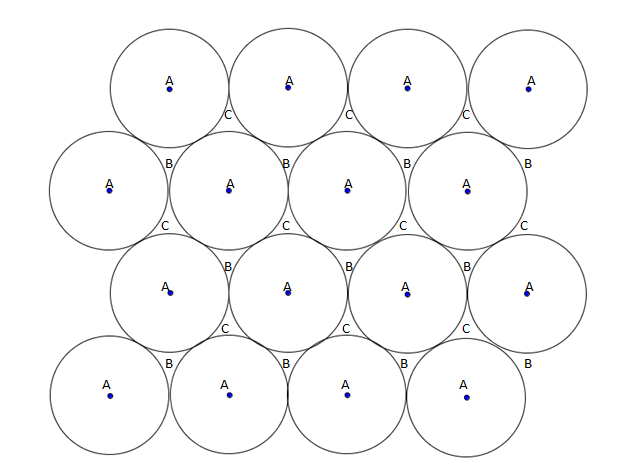
\includegraphics[width=10cm]{fcc}
\caption{Lagen $A$, $B$ en $C$ van de bolsapel}
\end{figure}


Het bewijs voor dit vermoeden bevatte geen berekeningen en was eigenlijk heel kort. Gauss zag dat wanneer 2 bollen elkaar raakten, het rooster ervoor zou zorgen dat een hele rij opeenvolgende bollen elkaar zou raken, waardoor evenwijdige rijen bollen zouden ontstaan. Wanneer deze rijen elkaar raakten, zouden zij het minst ruimte overlaten, als de middelpunten van drie bollen een gelijkzijdige driehoek vormden en zo verkreeg hij een oneindig aantal identieke vlakken met bollen die op de dichtste manier gestapeld waren. Uiteindelijk plaatste hij deze identieke vlakken boven elkaar op zo'n manier dat elke bol in een vlak raakte aan 3 bollen in het vlak erboven en 3 bollen in het vlak er onder. Hiermee verkreeg hij het dichtste bolstapelmodel in drie dimensies volgens een rooster en bewees hij dat de \textquoteleft face-centered cubic packing' de dichtste pakkingsmethode was volgens een rooster. Maar hij toonde hiermee niet aan dat de \textquoteleft face-centered cubic packing' de dichtste pakkingsmethode was van �lle soorten pakkingsmethodes. Op dit bewijs was het nog eens bijna 200 jaar wachten, maar in tussentijd werden wel nog andere dingen in verband met 'het probleem van Kepler' bewezen.

\subsubsection*{Voronoicellen %en Delaunay-sterren
}

In sectie \ref{axel} hebben we het reeds gehad over de Scandinavische wiskundige Axel Thue (1863-1922) die in 1892 een theorie over het tweedimensionale equivalent voor \textquoteleft het probleem van Kepler' waarin men zocht naar de dichtste pakkingsmethode voor cirkels in het vlak. Thue betegelde het vlak met identieke gelijkzijdige zeshoeken en tekende in elke zeshoek een cirkel op zo'n manier dat elke cirkel alle zijden van de zeshoek raakte. Hier werkte hij dus met de zogenaamde Voronoicellen.

Algemeen genomen is dit, zoals je ondertussen wel weet, een ruimtelijk gebied rond een bepaald punt $A$, waarbinnen alle punten dichter bij A liggen dan bij elk ander gegeven punt $B, C, D...$ Dit wil zeggen dat een willekeurig genomen punt in een Voronoicel dichter ligt bij het centrum dat in deze cel ligt dan bij een centrum uit om het even welke andere Voronoicel.
Bij drie dimensies is het construeren van een Voronoicel niet zo eenvoudig. Elke bol heeft een complex omhulsel waarbinnen elk punt dichter ligt tot het eigen bolcentrum dan tot om het even welk ander bolcentrum.
Bij de \textquoteleft face-centered cubic packing' is de Voronoicel een ruitvormige dodeca�der (een regelmatig twaalfvlak). Het vermoeden van Kepler kan dan bijgevolg ook aangetoond worden als men kan bewijzen dat deze ruitvormige dodeca�der de kleinste Voronoicel is bij het bolstapelen.

Deze begrippen spelen een belangrijke rol in het uiteindelijke bewijs van Kepler. Ze zorgen er immers voor dat het reusachtige werk, om de dichtheid van elke bolstapeling te bepalen, wordt beperkt tot een specifieke berekening die uitgevoerd kan worden met de computer. Men zal niet langer zoeken naar de hoeveelheid ruimte die bollen innemen in een stapeling. In de plaats daarvan zal men zoeken naar de kleinst mogelijke Voronoicel.


\subsubsection*{L�szlo Fejes T�th}
De persoon die als eerste suggereerde om Voronoicellen te gebruiken in het bewijs voor het bolstapelprobleem was L�szlo Fejes T�th. Deze Hongaarse wiskundige toonde hiernaast ook aan dat je het vermoeden van Kepler voor oneindig veel bollen kon bewijzen door het voor 50 bollen te bewijzen. Daarnaast ontdekte hij dat er maar 5000 mogelijke stapelingen meer meededen in de strijd om de compactste stapeling. 
T�th wist dat je aan de hand van Voronoicellen kon bewijzen welke van de 5000 stapelingen de grootste dichtheid had. Maar hij ondervond uit zijn onderzoeken dat de grenzen van deze cellen niet voldoende waren, waardoor er een correctieterm moest ingevoerd worden. T�th was de eerste wiskundige die een voorstel deed voor zo'n correctieterm (1953). Alleen bleef toen nog onduidelijk of T�th in zijn berekening met correctieterm alle mogelijke stapelingen had vervat. Het werd wel duidelijk dat Keplers probleem kon opgelost worden met een optimalisatieprogramma met een eindig aantal variabelen en dat dit met de computer zou moeten opgelost worden. Jammer genoeg had men in 1953 nog niet de computers van tegenwoordig, waardoor het nog even wachten was op het uiteindelijke 'bewijs' voor 'het probleem van Kepler'. 


\subsubsection*{Een verlaging van de bovengrens}
In tussentijd probeerden de wiskundigen wel om het vermoeden van Kepler op een andere manier te bewijzen. Zij deden dit door te kijken welke dichtheid er maximaal bereikt kan worden. Indien het hen zou lukken om deze bovengrens te verlagen tot 74.05\%  kon men Kepler bij verstek gelijk geven, aangezien de dichtheid die hij verkreeg \[\frac{\pi}{\sqrt{18}}= 0,74048048\dots\] was. Daardoor zou de grens tussen de dichtheid bij de face-centered cubic packing en de bovengrens zo klein zijn dat er geen betere pakking meer kon bestaan dan de face-centered cubic pakking.
Maar het verlagen van de bovengrens bleek moeilijker dan men dacht. In 1958 behaalde C.A.Rogers een waarde van 77.964\%. Enkele decennia later verkreeg Lindsey in 1986 een bovengrens van 77.844\% en slechts twee jaar later vond Muder een grens van 77.836\%. De meest recente bovengrens verkreeg Muder in 1993, maar die was nog steeds 77.3055\% wat niet zoveel beter was dan de vorige bovengrens en nog steeds ver van hetgeen Kepler vermoedde. 
We kunnen dus concluderen dat het verlagen van de bovengrens niet echt effici�nt was. Daarom gaan we er dan ook niet meer verder op in. 




\subsubsection*{Wu-Yi Hsiang}
Wu-Yi Hsiang is een wiskundige van de universiteit van Californi�, die plots in de zomer van 1988 in de krant verscheen met zijn  bewijs voor het vermoeden van Kepler. Jammer genoeg bleek na een eerste controle dat het bewijs vol blunders zat, waardoor Hsiang zijn werk moest herbekijken. Een jaar later publiceerde hij dan zijn gereviseerde bewijs, maar opnieuw bleken er nog hiaten aanwezig te zijn, waardoor het bewijs nog steeds ongeldig was. Hierna volgde er een lange strijd tussen Hsiang en zijn critici, waarbij argumenten en tegenargumenten voor het bewijs elkaar opvolgden. Maar jammer voor Hsiang aanvaardde de wiskundige gemeenschap het bewijs niet. Ook Thomas Hales die uiteindelijk zelf het bewijs zal leveren vond het bewijs van Hsiang nonsens. Zo blijkt immers uit ��n van de brieven van Hales aan Hsiang, waarin hij schrijft: 
\begin{quotation}"E�n aanname in uw tweede verhandeling treft me als fundamenteler en toch veel moeilijker te bewijzen dan de andere ... U stelt dat 'de beste (dat is: volumeminimaliserende) manier om een tweede laag toe te voegen is zoveel mogelijk gaten af te dekken...' Uw redenering lijkt me zwaar en doorslaggevend op die aanname te steunen, en desondanks zie ik nergens een zweem van bewijs."
\end{quotation}
In 1996 gaf een zekere Doug Muder een samenvatting van de toenmalige situatie rond het bewijs voor het vermoeden van Kepler. Hierin kwam hij tot verschillende conclusies. Ten eerste zei hij dat het geschrift van Hsiang hoogstens een schets is van het vermoeden van Kepler. Ten tweede ontdekte hij dat zelfs deze schets tekortkomingen bevat, doordat enkele wiskundigen meerdere tegenvoorbeelden voor cruciale stappen in het bewijs van Hsiang  gevonden hebben. Als conclusie vindt hij dat het werk rond het Kepler-vermoeden moet voortgezet worden alsof Hsiangs geschrift nooit heeft bestaan.


\subsubsection{Het bewijs voor \textquoteleft het probleem van Kepler'}

\subsubsection*{Thomas Hales en Samuel Ferguson}


\begin{wrapfigure}[7]{l}{3cm}
  \vspace{-10mm}
  \begin{center}
  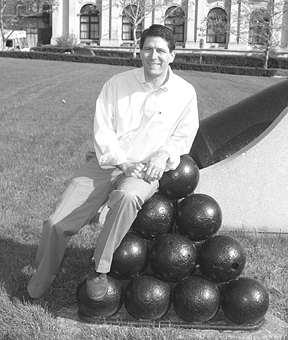
\includegraphics[width=3cm]{hales}\\
  Thomas Hales
  \end{center}
\end{wrapfigure}

Op 9 augustus 1998 kwam het einde voor het bewijs eindelijk in zicht. Thomas Hales, werkzaam aan de universiteit van Pittsburgh, Pennsylvania, stuurde toen een e-mail naar zijn collega's met het opluchtende nieuws dat hij het vermoeden van Kepler bewezen had.
\begin{quotation} "I have started to distribute copies of a series of papers giving a solution to the Kepler conjecture, the oldest problem in discrete geometry." 
\end{quotation} 
Hales toonde Keplers vermoeden aan in een reeks van artikelen die samen het complete bewijs vormen. In totaal gaat dit over 7 artikelen van Hales en een proefschrift van zijn doctoraatstudent, Samuel Ferguson, samen ongeveer 250 pagina's met daarbij 3 gigabytes aan computercode.
Om Keplers vermoeden te bewijzen, steunde Hales op een werk van L. Fejes T�th, waarin staat dat men slechts 5000 stapelingen moet controleren om het vermoeden van Kepler te bewijzen. Hales verdeelde deze 5000 stapelingen in 5 categorie�n waarvan hij er vier zelf bewees. De laatste categorie liet hij over aan Samuel Ferguson.


\subsubsection{Twijfels achteraf}
Ondanks dat alles dus achter de rug bleek te zijn, bleven sommige wiskundigen twijfelen aan de bewijsmethode van Hales. Zij mopperden dat deze brute aanpak met de computer niet echt \textquoteleft interessant' is, omdat men er niets van leert. Er zijn immers geen interessante denkstappen die men kan gebruiken voor andere onderzoeken.
Om de twijfelaars toch te overtuigen werd het gigantische computerprogramma van Hales gecontroleerd door twaalf mensen onder leiding van G�bor Fejes T�th, de zoon van de wiskundige op wie Hales zich baseerde. Na ongeveer 5 jaar kwamen de referees tot de slotsom dat het bewijs zeker voor 99\% klopte.
Maar er bleef toch nog een kleine marge open die twijfel bleef zaaien, waardoor men het bewijs van Hales en Ferguson publiceerde met een kleine kanttekening.

Omdat dit een tegenvaller was voor Hales, startte hij zelf een nieuw project om zijn bewijs formeel te controleren. Hierbij gebruikte hij opnieuw een computer om zijn computerprogramma door te lichten. Hales denkt dat dit project binnen de 20 jaar zal afgerond zijn. Als reactie op Hales zoekactie F*P*K (Formal Proof of the Kepler conjecture) ging ook het project Flyspeck van start.
Collega-wiskundigen spraken hun angst uit dat Hales teveel gebruik maakt van computers. Volgens hen zal de groeiende rol van de computers leiden tot wiskunde die onvatbaar zal zijn voor de mensen. Toch is Hales' bewijs niet de eerste wiskundige krachtmeting van de computer. Het bekendst is waarschijnlijk het vierkleurenprobleem, het probleem dat men minimaal vier kleuren nodig heeft om elke willekeurige landkaart zo in te kleuren dat er geen twee gebieden met dezelfde kleur aan elkaar grenzen. Dit is opgelost door een computerprogramma. Ook in het begin van onze lessenreeks zagen we een bewijs met behulp van de computer, namelijk dat de laagste orde voor een perfect vierkant 21 is.

\subsubsection{Conclusie}
Een eerste punt dat naar voor komt als je de evolutie van het bewijs van Kepler bekijkt, is het feit dat het bolstapelprobleem toch moeilijker is dan het lijkt. Ondanks dat men dus al decennia lang wist dat de face-centred cubic packing de meest compacte stapeling is, kon men dit vermoeden niet bewijzen. Het vermoeden van Kepler bleef dus eeuwen zonder bewijs. Het grootste probleem was het feit dat er enorm veel mogelijke stapelingen zijn, waarvan men niet wist welke nu de meest compacte was. Gelukkige kon Thomas Hales uiteindelijk de wiskundige gemeenschap verlossen met zijn bewijs.
Of toch niet? Want doordat Hales dit probleem met de computer bewezen heeft, laaide opnieuw de discussie op over de rol van de computer in bewijsvoeringen. De ene wiskundige vindt het goed dat er computers gebruikt worden, maar de andere denkt dat we op die manier te veel gehecht gaan geraken aan technologische hulpmiddelen, waardoor wiskundigen geen bewijzen meer zullen kunnen opstellen op de traditionele manuele manier. 

\ask{Wat vinden jullie van een bewijs met de computer?}
\question{Is deze vraag misschien te moeilijk voor kinderen van het middelbaar??}

Ondanks het bestaan van computers en alsmaar meer kennis blijven er echter nog veel problemen onopgelost. Er zijn nog veel nieuwe interessante dingen te ontdekken en uitdagingen aan te gaan. Daardoor blijft de wiskunde nog zeer actueel en levendig.

\newpage
%\section{Referenties}

\begin{thebibliography}{8}
\bibitem{1}\label{1} Hans Meissen en Rob van Oord, \textit{Schuiven met auto's, munten en bollen}, Epsilon Uitgaven, Utrecht, 2001-2002.
\bibitem{2}\label{2} Hans Lauwerier, \textit{Fractals, Meetkundige figuren in eindeloze herhaling}, Aramith Uitgevers, Bloemendaal, 1987.
\bibitem{3}\label{3} Miodrag S. Petkovi, \textit{Famous puzzles of great mathematicians}, American Mathematical Society, 2009.
\bibitem{4}\label{4} Keith Devlin, \textit{Wiskunde: Wetenschap van patronen en structuren}, Het Spectrum, 1998.
\bibitem{5}\label{5} Marcus du Sautoy, \textit{The Story of Maths}, BBC reeks, 2008.
\bibitem{6}\label{6} John J. O'Connor, Edmund F. Robertson, \textit{The MacTutor History of Mathematics archive}, \url{http://www-history.mcs.st-andrews.ac.uk/}
\bibitem{7}\label{7} Stuart Anderson, \textit{Squaring.Net}, \url{http://www.squaring.net/}
\bibitem{8}\label{8} Mike Askew, \textit{Meetkunde. Van $\pi$ tot Pythagoras}, Librero, 2011.
\bibitem{9}\label{9} http://www.luek.nl/illusie\_puzzle\_driehoek.php
\end{thebibliography}


\end{document}
